%_____________________________________________________________________________
%=============================================================================
% main.tex v10 (02-10-2016) \ldots dibuat oleh Lionov - Informatika FTIS UNPAR 
% 
% Ini adalah file utama (main.tex), berisi perintah-perintah yang khusus 
% dibuat untuk template ini
%
% 			JANGAN MENGUBAH APAPUN DI DALAM FILE INI, 
%			KECUALI ANDA TAHU APA YANG ANDA LAKUKAN !!! 
% 
% Perubahan pada versi 10 (02-10-2016):
%	- Perubahan nama file dari main.tex menjadi skripsi.tex
%	- Perubahan style bibliography dari "ieeetr" menjadi "compj" yang digunakan
%     di jurnal "The Computer Journal" yg diterbitkan oleh Oxford University 
%     Press/British Computer Society
%	- Penempatan gambar otomatis di folder "Gambar", jadi tidak perlu menuliskan
%	  nama folder lagi (\includegraphics{Gambar/tes} --> \includegraphics{tes})
%	- Perubahan font menjadi latin modern yg sdh banyak digunakan di jurnal2 intl
%   - Perbaikan kecil: jeda antara ttd pembimbing dan penguji
%	- Pembimbing Tunggal --> Pembimbing (karena sdh jelas tunggal 
%	- Penggunaan kantlipsum (output bhs inggris) sebagai pengganti lipsum
%	- \onespacing otomatis untuk buku skripsi final, untuk buku sidang tetap 
%	  \onehalfspacing
%	- Perbaikan hfill dan hfil yang masih menjadi masalah, bagian itu dipindahkan
%	  ke dekat deklarasi Daftar Isi
%_____________________________________________________________________________
%=============================================================================

%setup.tex
\documentclass[11pt,a4paper,twoside,openright,notitlepage]{report}  

\usepackage{lmodern} %font latin modern 
\usepackage[bahasa]{babel} %bahasa indonesia
\usepackage[T1]{fontenc}  %encoding
% \usepackage{mathptmx}
% \usepackage{venturisold}
% \usepackage{helvet}
% \usepackage{fouriernc} 
\usepackage{abstract} %manipulasi abstract
\usepackage{chappg} % format daftar isi 
\usepackage{color} %warna 
\usepackage{etoolbox} %untuk programming if-then
\usepackage{fancyhdr} %format header & footer
\usepackage{float} %penempatan gambar di tempat yg seharusnya 
\usepackage[inner=2.5cm,outer=2cm,top=2.5cm,bottom=2.5cm]{geometry} %margin
\usepackage{graphicx} %gambar
\usepackage{listings} %source code
\usepackage{lscape} %landscape untuk source code
\usepackage{multicol} %multiple column
\usepackage{ifthen} % if then
\usepackage[pagewise]{lineno} %line numbering
\usepackage{kantlipsum} % untuk dummy text
\usepackage{titlesec} %judul header
\usepackage{tocbibind} %daftar isi, gambar, tabel dll
\usepackage{tocloft} % format daftar isi 
\usepackage{setspace} %line spacing
\usepackage{xstring} %manipulasi string
\usepackage[plainpages=false,pdfpagelabels,unicode]{hyperref} %\autoref, \phantomsection & link 
\usepackage{emptypage} %halaman kosong antar bab
\graphicspath{{./Gambar/}} 

\usepackage{lcg}
\newcommand{\random}{\rand\arabic{rand}}

\let\abstractname\Abstrak

\normalfont
\DeclareFontShape{T1}{lmr}{bx}{sc} { <-> ssub * cmr/bx/sc }{}

\titleformat{\chapter}[display] {\Large\bfseries\centering}{\MakeUppercase{\chaptertitlename} \thechapter}{15pt}{\Large\MakeUppercase}

\renewcommand{\cftchapfont}{\scshape \bfseries}

% Tidak perlu ada kata "Bab", "Gambar" atau "Tabel" di daftar 
% \renewcommand{\cftchappresnum}{{\bf \scshape Bab} } 
% \renewcommand{\cftchapnumwidth}{1.5cm}
% \renewcommand{\cftfigpresnum}{{Gambar\ }} 
% \renewcommand{\cftfignumwidth}{2.5cm}
% \renewcommand{\cfttabpresnum}{{Tabel\ }} 
% \renewcommand{\cfttabnumwidth}{2cm}


\newcommand{\vnama}{Jane Doe}
\newcommand{\vlnama}{John Doe}
\newcommand{\vnpm}{1992700001}
\newcommand{\vprodiINA}{SAINS}
\newcommand{\vprodiENG}{SCIENCE}
\newcommand{\vstaINA}{UJIAN}
\newcommand{\vstaENG}{EXAM}
%\newcommand{\vjudul}{Judul Skripsi/Tugas Akhir}
\newcommand{\vpembu}{Plato}
\newcommand{\vpembs}{Euclid}
\newcommand{\vpengi}{Plato}
\newcommand{\vpengii}{Euclid}
\newcommand{\vtanggal}{1}
\newcommand{\vbulan}{Januari}
\newcommand{\vtahun}{1970}
\newcommand{\vmode}{final}
\newcommand{\vspacing}{double}
\newcommand{\vlineno}{yes}
\newcommand{\vkunciina}{Skripsi, Tugas Akhir}
\newcommand{\vkuncieng}{Undergraduate Thesis, Final Project}
\newcommand{\vkajur}{Jack Doe}
\newcommand{\vkajurmat}{Jack Doe}
\newcommand{\vkajurfis}{Jack Doe}
\newcommand{\vkajurtif}{Jack Doe}
\newcommand{\vtabel}{}
\newcommand{\vgambar}{}
\newcommand{\vdierror}{}

\newcommand{\namanpm}[2]{
	\renewcommand{\vstaINA}{<<SKRIPSI/TUGAS AKHIR>>}
	\renewcommand{\vprodiINA}{<<MATEMATIKA/FISIKA/TEKNIK INFORMATIKA>>}
	\renewcommand{\vstaENG}{<<FINAL PROJECT/UNDERGRADUATE THESIS>>}
	\renewcommand{\vprodiENG}{<<MATHEMATICS/PHYSICS/INFORMATICS>>}
	\renewcommand{\vnama}{\uppercase{#1}} \renewcommand{\vlnama}{#1} \hypersetup{pdfauthor={#2 - #1}}
	\renewcommand{\vnpm}{#2} \hypersetup{pdfcreator={#2}} \StrChar{\vnpm}{6}[\vprodiN]
%	\renewcommand{\vnpm}{#2} \hypersetup{pdfcreator={\jobname}} \StrChar{\vnpm}{6}[\vprodiN]
	\ifdefstring{\vprodiN}{1}{
		\renewcommand{\vprodiINA}{MATEMATIKA} \renewcommand{\vprodiENG}{MATHEMATICS} 
		\renewcommand{\vstaINA}{SKRIPSI} \renewcommand{\vstaENG}{FINAL PROJECT} \renewcommand{\vkajur}{\vkajurmat}}{}
	\ifdefstring{\vprodiN}{2}{
		\renewcommand{\vprodiINA}{FISIKA} \renewcommand{\vprodiENG}{PHYSICS} 
		\renewcommand{\vstaINA}{TUGAS AKHIR} \renewcommand{\vstaENG}{FINAL PROJECT} \renewcommand{\vkajur}{\vkajurfis}}{}
	\ifdefstring{\vprodiN}{3}{
		\renewcommand{\vprodiINA}{TEKNIK INFORMATIKA} \renewcommand{\vprodiENG}{INFORMATICS} 
		\renewcommand{\vstaINA}{SKRIPSI} \renewcommand{\vstaENG}{UNDERGRADUATE THESIS} \renewcommand{\vkajur}{\vkajurtif}}{}
	}

%\newcommand{\judul}[1]{\renewcommand{\vjudul}{\uppercase{#1}}\hypersetup{pdftitle={#1}, pdfsubject={#1}}}
\newcommand{\pembimbing}[2]{\renewcommand{\vpembu}{#1}\renewcommand{\vpembs}{#2}}
\newcommand{\penguji}[2]{\renewcommand{\vpengi}{#1}\renewcommand{\vpengii}{#2}}
\newcommand{\kajur}[3]{\renewcommand{\vkajurmat}{#1}\renewcommand{\vkajurfis}{#2}\renewcommand{\vkajurtif}{#3}}
\renewcommand{\vbulan}{<<bulan>>}
\newcommand{\tanggal}[3]{\renewcommand{\vtanggal}{#1}\renewcommand{\vtahun}{#3}
	\newcommand{\vcbulan}{#2}
	\ifdefstring{\vcbulan}{1}{\renewcommand{\vbulan}{Januari}}{}
	\ifdefstring{\vcbulan}{2}{\renewcommand{\vbulan}{Februari}}{}
	\ifdefstring{\vcbulan}{3}{\renewcommand{\vbulan}{Maret}}{}
	\ifdefstring{\vcbulan}{4}{\renewcommand{\vbulan}{April}}{}
	\ifdefstring{\vcbulan}{5}{\renewcommand{\vbulan}{Mei}}{}
	\ifdefstring{\vcbulan}{6}{\renewcommand{\vbulan}{Juni}}{}
	\ifdefstring{\vcbulan}{7}{\renewcommand{\vbulan}{Juli}}{}
	\ifdefstring{\vcbulan}{8}{\renewcommand{\vbulan}{Agustus}}{}
	\ifdefstring{\vcbulan}{9}{\renewcommand{\vbulan}{September}}{}
	\ifdefstring{\vcbulan}{10}{\renewcommand{\vbulan}{Oktober}}{}
	\ifdefstring{\vcbulan}{11}{\renewcommand{\vbulan}{November}}{}
	\ifdefstring{\vcbulan}{12}{\renewcommand{\vbulan}{Desember}}{}	
}

\newcommand{\judulINA}[1]{\newcommand{\vjudulINA}{\uppercase{#1}}\hypersetup{pdftitle={#1},pdfsubject={#1}}}
\newcommand{\judulENG}[1]{\newcommand{\vjudulENG}{\uppercase{#1}}\hypersetup{pdftitle={#1},pdfsubject={#1}}}
\newcommand{\abstrakINA}[1]{\newcommand{\vabstrakina}{#1}}
\newcommand{\abstrakENG}[1]{\newcommand{\vabstrakeng}{#1}}
\newcommand{\kunciINA}[1]{\renewcommand{\vkunciina}{#1} \hypersetup{pdfkeywords={#1}}}
\newcommand{\kunciENG}[1]{\renewcommand{\vkuncieng}{#1}}
\newcommand{\untuk}[1]{\newcommand{\vuntuk}{#1}}
\newcommand{\prakata}[1]{\newcommand{\vprakata}{#1}}
\newcommand{\mode}[1]{\renewcommand{\vmode}{#1}}
\newcommand{\linespacing}[1]{\renewcommand{\vspacing}{#1}}
\newcommand{\linenumber}[1]{\renewcommand{\vlineno}{#1}}

\newcommand{\daftarIsiError}[1]{\renewcommand{\vdierror}{#1}} 
\newcommand{\gambar}[1]{\renewcommand{\vgambar}{#1}}
\newcommand{\tabel}[1]{\renewcommand{\vtabel}{#1}}

\newcommand{\bab}[1]{\newcommand{\vbab}{#1}}
\newcommand{\lampiran}[1]{\renewcommand{\vlmp}{#1}} 

\newcommand{\vpilbab}{0}
\newcommand{\vbaba}{0}\newcommand{\vbabb}{0}\newcommand{\vbabc}{0}
\newcommand{\vbabd}{0}\newcommand{\vbabe}{0}\newcommand{\vbabf}{0}
\newcommand{\vbabg}{0}\newcommand{\vbabh}{0}\newcommand{\vbabi}{0}
\newcommand{\vpillmp}{0}
\newcommand{\vlmpa}{0}\newcommand{\vlmpb}{0}\newcommand{\vlmpc}{0}
\newcommand{\vlmpd}{0}\newcommand{\vlmpe}{0}\newcommand{\vlmpf}{0}
\newcommand{\vlmpg}{0}\newcommand{\vlmph}{0}\newcommand{\vlmpi}{0}
\newcommand{\vlmp}{x}

%	\ifdefempty{#1}{\bab{1,2,3,4,5,6,7,8,9} \tampilbab{\vbab}}{
\newcommand{\tampilbab}[1]{
	\ifdefempty{#1}{
		\renewcommand{\vbaba}{1}\renewcommand{\vbabb}{1}\renewcommand{\vbabc}{1}
		\renewcommand{\vbabd}{1}\renewcommand{\vbabe}{1}\renewcommand{\vbabf}{1}
		\renewcommand{\vbabg}{1}\renewcommand{\vbabh}{1}\renewcommand{\vbabi}{1}}{
	\renewcommand{\do}[1]{
		\renewcommand{\vpilbab}{##1}
		\ifdefstring{\vpilbab}{1}{\renewcommand{\vbaba}{1}}{}
		\ifdefstring{\vpilbab}{2}{\renewcommand{\vbabb}{1}}{}
		\ifdefstring{\vpilbab}{3}{\renewcommand{\vbabc}{1}}{}
		\ifdefstring{\vpilbab}{4}{\renewcommand{\vbabd}{1}}{}
		\ifdefstring{\vpilbab}{5}{\renewcommand{\vbabe}{1}}{}
		\ifdefstring{\vpilbab}{6}{\renewcommand{\vbabf}{1}}{}
		\ifdefstring{\vpilbab}{7}{\renewcommand{\vbabg}{1}}{}
		\ifdefstring{\vpilbab}{8}{\renewcommand{\vbabh}{1}}{}
		\ifdefstring{\vpilbab}{9}{\renewcommand{\vbabi}{1}}{}
	}
	\expandafter\docsvlist\expandafter{#1}
	}
}

\newcommand{\tampillmp}[1]{
	\ifdefempty{#1}{
		\renewcommand{\vlmpa}{1}\renewcommand{\vlmpb}{1}\renewcommand{\vlmpc}{1}
		\renewcommand{\vlmpd}{1}\renewcommand{\vlmpe}{1}\renewcommand{\vlmpf}{1}
		\renewcommand{\vlmpg}{1}\renewcommand{\vlmph}{1}\renewcommand{\vlmpi}{1}}{
	\ifdefstring{#1}{-1}{ }{
		\renewcommand{\do}[1]{ 
			\renewcommand{\vpillmp}{##1}
			\ifdefstring{\vpillmp}{A}{\renewcommand{\vlmpa}{1}}{}
			\ifdefstring{\vpillmp}{B}{\renewcommand{\vlmpb}{1}}{}
			\ifdefstring{\vpillmp}{C}{\renewcommand{\vlmpc}{1}}{}
			\ifdefstring{\vpillmp}{D}{\renewcommand{\vlmpd}{1}}{}
			\ifdefstring{\vpillmp}{E}{\renewcommand{\vlmpe}{1}}{}
			\ifdefstring{\vpillmp}{F}{\renewcommand{\vlmpf}{1}}{}
			\ifdefstring{\vpillmp}{G}{\renewcommand{\vlmpg}{1}}{}
			\ifdefstring{\vpillmp}{H}{\renewcommand{\vlmph}{1}}{}
			\ifdefstring{\vpillmp}{I}{\renewcommand{\vlmpi}{1}}{}}
		}
	\expandafter\docsvlist\expandafter{#1}
	}
}

\newcommand{\appspacing}{
	\ifdefstring{\vspacing}{single}{\singlespacing}{}
	\ifdefstring{\vspacing}{onehalf}{\onehalfspacing}{}
	\ifdefstring{\vspacing}{double}{\doublespacing}{}
	\ifdefstring{\vmode}{sidang}{\onehalfspacing}{}	
	\ifdefstring{\vmode}{sidang_akhir}{\onehalfspacing}{}	
	\ifdefstring{\vmode}{final}{\singlespacing}{}
}

\newcommand{\appline}{
	\ifdefstring{\vmode}{final}{\renewcommand{\vlineno}{no}}{}
	\ifdefstring{\vlineno}{yes}{\linenumbers \def\linenumberfont{\normalfont\tiny\sffamily}}{}
	\ifdefstring{\vlineno}{no}{\lstset{numbers=left, stepnumber=1, numbersep=5pt}}{}
	
}

\newcommand{\appmargin}{
	\ifdefstring{\vmode}{final}{}{\newgeometry{inner=3cm,outer=2.75cm,top=2cm,bottom=2cm}}
}

\renewcommand{\abstractnamefont}{\bf \MakeUppercase}

\makeatletter
\def\headrule{{%
  \if@fancyplain\let\headrulewidth\plainheadrulewidth\fi
  \hrule\@height\footrulewidth\@width\headwidth\vskip2pt%
  \hrule\@height\headrulewidth\@width\headwidth\vskip-\headrulewidth\vskip-4pt
}}
\def\footrule{}

\def\cleardoublepage{
	\clearpage
	\if@twoside \ifodd\c@page
	\else
		\hbox{}
		\vspace{\fill} 
		\thispagestyle{empty}
		\newpage
	\if@twocolumn\hbox{}\newpage\fi\fi\fi}
\makeatother

\renewcommand{\headrulewidth}{1.25pt}
\renewcommand{\footrulewidth}{0.25pt}

\setlength{\headheight}{15pt}
\fancyhead[LE,RO]{\thepage}
\fancyhead[RE]{\small{\textsc{\nouppercase{\leftmark}}}}
\fancyhead[LO]{\small{\textsc{\nouppercase{\rightmark}}}}
\fancyfoot{}

\hypersetup{unicode=true,colorlinks=true,linkcolor=blue,citecolor=green,filecolor=magenta, urlcolor=cyan}

\lstset{basicstyle=\tiny, commentstyle=\color{blue}}
\lstset{frame=leftline, tabsize=4, breaklines=true}

%end setup.tex

%_____________________________________________________________________________
%=============================================================================
% data.tex v8 (02-10-2016) \ldots dibuat oleh Lionov - Informatika FTIS UNPAR
%
% Perubahan pada versi 8 (02-10-2016)
%	- Perubahan keterangan pada spacing: Otomatis spasi 1 untuk buku skripsi 
%	  final dan 1.5 untuk buku sidang
%	- Penggunaan kantlipsum
%_____________________________________________________________________________
%=============================================================================

%=============================================================================
% 								PETUNJUK
%=============================================================================
% Ini adalah file data (data.tex)
% Masukkan ke dalam file ini, data-data yang diperlukan oleh template ini
% Cara memasukkan data dijelaskan di setiap bagian
% Data yang WAJIB dan HARUS diisi dengan baik dan benar adalah SELURUHNYA !!
% Hilangkan tanda << dan >> jika anda menemukannya
%=============================================================================

%_____________________________________________________________________________
%=============================================================================
% 								BAGIAN 0
%=============================================================================
% PERHATIAN!! PERHATIAN!! Bagian ini hanya ada untuk sementara saja
% Jika "DAFTAR ISI" tidak bisa berada di bagian tengah halaman, isi dengan XXX
% jika sudah benar posisinya, biarkan kosong (i.e. \daftarIsiError{ })
%=============================================================================
\daftarIsiError{ }
%=============================================================================

%_____________________________________________________________________________
%=============================================================================
% 								BAGIAN I
%=============================================================================
% Tambahkan package2 lain yang anda butuhkan di sini
%=============================================================================
\usepackage{booktabs} 
\usepackage[table]{xcolor}
\usepackage{longtable}
\usepackage{amssymb}
\usepackage{todo}
\usepackage{verbatim} 		%multilne comment
\usepackage{pgfplots}
%=============================================================================

%_____________________________________________________________________________
%=============================================================================
% 								BAGIAN II
%=============================================================================
% Mode dokumen: menetukan halaman depan dari dokumen, apakah harus mengandung 
% prakata/pernyataan/abstrak dll (termasuk daftar gambar/tabel/isi) ?
% - kosong : tidak ada halaman depan sama sekali (untuk dokumen yang 
%            dipergunakan pada proses bimbingan)
% - cover : cover saja tanpa daftar isi, gambar dan tabel
% - sidang : cover, daftar isi, gambar, tabel 
% - sidang_akhir : mode sidang + abstrak + abstract
% - final : seluruh halaman awal dokumen (untuk cetak final)
% Jika tidak ingin mencetak daftar tabel/gambar (misalkan karena tidak ada 
% isinya), edit manual di baris 439 dan 440 pada file main.tex
%=============================================================================
% \mode{kosong}
% \mode{cover}
% \mode{sidang}
% \mode{sidang_akhir}
 \mode{final} 
%=============================================================================

%_____________________________________________________________________________
%=============================================================================
% 								BAGIAN III
%=============================================================================
% Line numbering: penomoran setiap baris, otomatis di-reset setiap berganti
% halaman
% - yes: setiap baris diberi nomor
% - no : baris tidak diberi nomor, otomatis untuk mode final
%=============================================================================
\linenumber{no}
%=============================================================================

%_____________________________________________________________________________
%=============================================================================
% 								BAGIAN IV
%=============================================================================
% Linespacing: jarak antara baris 
% - single	: wajib (dan otomatis jika ingin mencetak buku skripsi, opsi yang 
%			  disediakan untuk bimbingan, jika pembimbing tidak keberatan 
%			  (untuk menghemat kertas)
% - onehalf	: default dan wajib (dan otomatis) jika ingin mencetak dokumen
%             untuk sidang.
% - double 	: jarak yang lebih lebar lagi, jika pembimbing berniat memberi 
%             catatan yg banyak di antara baris (dianjurkan untuk bimbingan)
%=============================================================================
\linespacing{single}
%\linespacing{onehalf}
%\linespacing{double}
%=============================================================================

%_____________________________________________________________________________
%=============================================================================
% 								BAGIAN V
%=============================================================================
% Tidak semua skripsi memuat gambar dan/atau tabel. Untuk skripsi yang seperti
% itu, tidak diperlukan Daftar Gambar dan Daftar Tabel. Sayangnya hal ini 
% sulit dilakukan secara manual karena membutuhkan kedisiplinan pengguna 
% template.  
% Jika tidak akan menampilkan Daftar Gambar/Tabel, isi dengan NO. Jika ingin
% menampilkan, kosongkan parameter (i.e. \gambar{ }, \tabel{ })
%=============================================================================
\gambar{ }
\tabel{ }
%=============================================================================

%_____________________________________________________________________________
%=============================================================================
% 								BAGIAN VI
%=============================================================================
% Bab yang akan dicetak: isi dengan angka 1,2,3 s.d 9, sehingga bisa digunakan
% untuk mencetak hanya 1 atau beberapa bab saja
% Jika lebih dari 1 bab, pisahkan dengan ',', bab akan dicetak terurut sesuai 
% urutan bab (e.g. \bab{1,2,3}).
% Untuk mencetak seluruh bab, kosongkan parameter (i.e. \bab{ })  
% Catatan: Jika ingin menambahkan bab ke-10 dan seterusnya, harus dilakukan 
% secara manual
%=============================================================================
\bab{ }
%=============================================================================

%_____________________________________________________________________________
%=============================================================================
% 								BAGIAN VII
%=============================================================================
% Lampiran yang akan dicetak: isi dengan huruf A,B,C s.d I, sehingga bisa 
% digunakan untuk mencetak hanya 1 atau beberapa lampiran saja
% Jika lebih dari 1 lampiran, pisahkan dengan ',', lampiran akan dicetak 
% terurut sesuai urutan lampiran (e.g. \bab{A,B,C}).
% Jika tidak ingin mencetak lampiran apapun, isi dengan -1 (i.e. \lampiran{-1})
% Untuk mencetak seluruh mapiran, kosongkan parameter (i.e. \lampiran{ })  
% Catatan: Jika ingin menambahkan lampiran ke-J dan seterusnya, harus 
% dilakukan secara manual
%=============================================================================
\lampiran{ }
%=============================================================================

%_____________________________________________________________________________
%=============================================================================
% 								BAGIAN VIII
%=============================================================================
% Data diri dan skripsi/tugas akhir
% - namanpm: Nama dan NPM anda, penggunaan huruf besar untuk nama harus benar
%			 dan gunakan 10 digit npm UNPAR, PASTIKAN BAHWA BENAR !!!
%			 (e.g. \namanpm{Jane Doe}{1992710001}
% - judul : Dalam bahasa Indonesia, perhatikan penggunaan huruf besar, judul
%			tidak menggunakan huruf besar seluruhnya !!! 
% - tanggal : isi dengan {tangga}{bulan}{tahun} dalam angka numerik, jangan 
%			  menuliskan kata (e.g. AGUSTUS) dalam isian bulan
%			  Tanggal ini adalah tanggal dimana anda akan melaksanakan sidang 
%			  ujian akhir skripsi/tugas akhir
% - pembimbing: isi dengan pembimbing anda, lihat daftar dosen di file dosen.tex
%				jika pembimbing hanya 1, kosongkan parameter kedua 
%				(e.g. \pembimbing{\JND}{  } ) , \JND adalah kode dosen
% - penguji : isi dengan para penguji anda, lihat daftar dosen di file dosen.tex
%				(e.g. \penguji{\JHD}{\JCD} ) , \JND dan \JCD adalah kode dosen
% !!Lihat singkatan pembimbing dan penguji anda di file dosen.tex
%=============================================================================
\namanpm{Michael Adrian}{2013730039}	%hilangkan tanda << & >>
\tanggal{<<tanggal>>}{<<bulan>>}{2017}				%hilangkan tanda << & >>
\pembimbing{\CEN}{<<pembimbing 2>>} %hilangkan tanda << & >>
\penguji{<<penguji 1>>}{<<penguji 2>>} 				%hilangkan tanda << & >>
%=============================================================================

%_____________________________________________________________________________
%=============================================================================
% 								BAGIAN IX
%=============================================================================
% Judul dan title : judul bhs indonesia dan inggris
% - judulINA: judul dalam bahasa indonesia
% - judulENG: title in english
% PERHATIAN: - langsung mulai setelah '{' awal, jangan mulai menulis di baris 
%			   bawahnya
%			 - Gunakan \texorpdfstring{\\}{} untuk pindah ke baris baru
%			 - Judul TIDAK ditulis dengan menggunakan huruf besar seluruhnya !!
%			 - Gunakan perintah \texorpdfstring{\\}{} untuk baris baru
%=============================================================================
\judulINA{Perbandingan Algoritma Backtracking dengan Algoritma Hybrid Genetic untuk Menyelesaikan Permainan Calcudoku}
\judulENG{Comparison of the Backtracking Algorithm and the Hybrid Genetic Algorithm to Solve the Calcudoku Puzzle}
%_____________________________________________________________________________
%=============================================================================
% 								BAGIAN X
%=============================================================================
% Abstrak dan abstract : abstrak bhs indonesia dan inggris
% - abstrakINA: abstrak bahasa indonesia
% - abstrakENG: abstract in english
% PERHATIAN: langsung mulai setelah '{' awal, jangan mulai menulis di baris 
%			 bawahnya
%=============================================================================
\abstrakINA
{Calcudoku adalah sebuah permainan teka-teki angka. Tujuan dari teka-teki ini adalah mengisi setiap sel dalam \textit{grid} dengan angka 1 sampai \begin{math}n\end{math} tanpa pengulangan angka dalam setiap kolomnya dan barisnya untuk \textit{grid} berukuran \begin{math}n \times n\end{math}. \textit{Grid} ini dibagi menjadi sejumlah \textit{cage} dengan setiap \textit{cage} yang jumlah selnya bervariasi. Setiap \textit{cage} dibatasi oleh garis yang lebih tebal daripada garis pembatas antar sel. Angka-angka dalam satu \textit{cage} yang sama harus menghasilkan angka tujuan yang telah ditentukan jika dihitung menggunakan operasi matematika yang ditentukan. Angka-angka dalam satu \textit{cage} juga boleh berulang, selama pengulangan tidak terjadi dalam satu kolom atau baris yang sama.

Dua algoritma telah terbukti berhasil dalam menyelesaikan Calcudoku, yaitu algoritma \textit{backtracking} dan algoritma \textit{hybrid genetic}.

Algoritma \textit{backtracking} adalah sebuah algoritma umum yang mencari solusi dengan mencoba salah satu dari beberapa pilihan, jika pilihan yang dipilih ternyata salah, komputasi dimulai lagi pada titik pilihan dan mencoba pilihan lainnya.

Algoritma \textit{hybrid genetic} dalam kasus ini adalah gabungan dari algoritma \textit{rule based} dan algoritma genetik. Algoritma \textit{rule based} adalah sebuah algoritma berbasis aturan logika untuk menyelesaikan Calcudoku. Algoritma genetik adalah salah satu teknik heuristik \textit{Generate and Test} yang terinspirasi oleh sistem seleksi alam yang mencari solusi dengan menggunakan operator-operator genetik seperti mutasi, kawin silang, dan \textit{elitism}.

Penelitian ini bertujuan untuk membandingkan performansi algoritma \textit{backtracking} dengan algoritma \textit{hybrid genetic} dalam menyelesaikan Calcudoku dalam kecepatan dan tingkat keberhasilan.}
\abstrakENG
{Calcudoku is a number puzzle game. The goal of this puzzle is to fill each cell in the grid with the numbers from 1 to n without repetitions of the numbers in each column and row for grid with the size of n x n. The grid is divided into a number of cages, with each cage contains a variable number of cells. Each cage is bordered with a thicker line than cell border line. Numbers in the same cage must produced the predetermined target number if calculated using the predetermined mathematical operatin. Numbers in a cage can be repeated, as long as the repetitions do not occur in the same column or row.

Two algorithms have been proven to successfully solve Calcudoku. The two algorithms are the backtracking algorithm and the hybrid genetic algorithm.

The backtracking algorithm is a general algorithm with finds a solution by trying one of several choices, if the choice proves to be incorrect, the computation restarts at the point of choice and tries another choice.

In this case, the hybrid genetic algorithm is a combination of the rule based algorithm and the genetic algorithm. Rule based algorithm uses logical rules to solve Calcudoku. Genetic algorithm is a heuristic technique inspired by the process of natural selection, which tries to find a solution by relying on genetic operators such as mutation, crossover, and elitism.

The goal of this research is to compare the backtracking algorithm and the hybrid genetic in solving Calcudoku in speed and success rate.}
%=============================================================================

%_____________________________________________________________________________
%=============================================================================
% 								BAGIAN XI
%=============================================================================
% Kata-kata kunci dan keywords : diletakkan di bawah abstrak (ina dan eng)
% - kunciINA: kata-kata kunci dalam bahasa indonesia
% - kunciENG: keywords in english
%=============================================================================
\kunciINA{Calcudoku, algoritma \textit{backtracking}, algoritma \textit{hybrid genetic}, algoritma \textit{rule based}, \textit{algoritma genetik}}
\kunciENG{Calcudoku, backtracking algorithm, hybrid genetic algorithm, rule based algorithm, genetic algorithm}
%=============================================================================

%_____________________________________________________________________________
%=============================================================================
% 								BAGIAN XII
%=============================================================================
% Persembahan : kepada siapa anda mempersembahkan skripsi ini ...
%=============================================================================
\untuk{Lorem ipsum dolor sit amet, consectetur adipiscing elit.}
%=============================================================================

%_____________________________________________________________________________
%=============================================================================
% 								BAGIAN XIII
%=============================================================================
% Kata Pengantar: tempat anda menuliskan kata pengantar dan ucapan terima 
% kasih kepada yang telah membantu anda bla bla bla ....  
%=============================================================================
\prakata
{Lorem ipsum dolor sit amet, consectetuer adipiscing elit, sed diam 
nonummy nibh euismod tincidunt ut laoreet dolore magna aliquam erat 
volutpat. Ut wisi enim ad minim veniam, quis nostrud exerci tation 
ullamcorper suscipit lobortis nisl ut aliquip ex ea commodo consequat. 
Duis autem vel eum iriure dolor in hendrerit in vulputate velit esse 
molestie consequat, vel illum dolore eu feugiat nulla facilisis at vero 
eros et accumsan et iusto odio dignissim qui blandit praesent luptatum 
zzril delenit augue duis dolore te feugait nulla facilisi. Nam liber 
tempor cum soluta nobis eleifend option congue nihil imperdiet doming 
id quod mazim placerat facer possim assum. Typi non habent claritatem 
insitam; est usus legentis in iis qui facit eorum claritatem. 
Investigationes demonstraverunt lectores legere me lius quod ii legunt 
saepius. Claritas est etiam processus dynamicus, qui sequitur 
mutationem consuetudium lectorum. Mirum est notare quam littera 
gothica, quam nunc putamus parum claram, anteposuerit litterarum formas 
humanitatis per seacula quarta decima et quinta decima. Eodem modo 
typi, qui nunc nobis videntur parum clari, fiant sollemnes in futurum.

Lorem ipsum dolor sit amet, consectetur adipiscing elit, sed do eiusmod 
tempor incididunt ut labore et dolore magna aliqua. Ut enim ad minim 
veniam, quis nostrud exercitation ullamco laboris nisi ut aliquip ex ea 
commodo consequat. Duis aute irure dolor in reprehenderit in voluptate 
velit esse cillum dolore eu fugiat nulla pariatur. Excepteur sint 
occaecat cupidatat non proident, sunt in culpa qui officia deserunt 
mollit anim id est laborum.}
%=============================================================================

%_____________________________________________________________________________
%=============================================================================
% 								BAGIAN XIV
%=============================================================================
% Tambahkan hyphen (pemenggalan kata) yang anda butuhkan di sini 
%=============================================================================
\hyphenation{ma-te-ma-ti-ka}
\hyphenation{fi-si-ka}
\hyphenation{tek-nik}
\hyphenation{in-for-ma-ti-ka}
\hyphenation{cal-cu-do-ku}
\hyphenation{al-go-rit-ma}
\hyphenation{back-track-ing}
\hyphenation{hy-brid}
\hyphenation{ge-ne-tic}
%=============================================================================

%_____________________________________________________________________________
%=============================================================================
% 								BAGIAN XV
%=============================================================================
% Tambahkan perintah yang anda buat sendiri di sini 
%=============================================================================
\newcommand{\vtemplateauthor}{lionov}
\pgfplotsset{compat=newest}
\usetikzlibrary{patterns}
%=============================================================================

% Copyright \textcopyright [Lionov] [09-10-2016]. All rights reserved
%_____________________________________________________________________________
%=============================================================================
% dosen.tex v7 (28-01-2017) dibuat oleh Lionov - T. Informatika FTIS UNPAR
%
% Perubahan pada versi 7 (28-01-2017)
%	- kaprodi (sebelumnya kajur) dan dideklarasikan di skripsi.tex
%	- memisahkan kaprodi per prodi
%	- menghapus dummy
%   - perubahan gelar untuk BNY
%_____________________________________________________________________________
%=============================================================================

%=============================================================================
% Data dosen dan kaprodi FTIS - JANGAN MENGUBAH APAPUN DI BAGIAN INI, KECUALI
% untuk mengubah kaprodi (jika kaprodi telah berganti orang) atau menambahkan 
% pembimbing anda yang tidak/belum tercantum pada daftar ini atau 
% memperbaiki penulisan gelar jika penguji anda meminta
%=============================================================================
%  CATATAN UNTUK MAHASISWA TEKNIK INFORMATIKA :
% dosen yang ditandai * :
% - jika menjadi pembimbing : harus diganti, penggantinya mengikuti petunjuk
% 	dari koordinator Skripsi !
% - jika menjadi penguji: tidak diganti, tetapi hapus komentar dan '*' agar 
%   dapat digunakan
%=============================================================================


%\kaprodi{\JDL}{\PNG}{\MTA} 
\renewcommand{\kaprodiMAT}{\JDL}
\renewcommand{\kaprodiFIS}{\PNG}
\renewcommand{\kaprodiTIF}{\MTA}

% Dosen-dosen Program Studi Matematika
\newcommand{\JDL}{Dr.\,Julius\,Dharma\,Lesmono}
\newcommand{\FAR}{Farah\,Kristiani,\,M.Si.}
\newcommand{\ERW}{Erwinna\,Chendra,\,M.Si.}
\newcommand{\FJP}{Dr.\,Ferry\,Jaya\,Permana,\,ASAI}
\newcommand{\AGS}{Agus\,Sukmana,\,M.Sc.}
\newcommand{\WSB}{Prof.\,M.\,Wono\,Setya\,Budhi,\,Ph.D.}
\newcommand{\LIM}{Liem\,Chin,\,M.Si.}
\newcommand{\IWS}{Iwan\,Sugiarto,\,M.Si.}
\newcommand{\IVM}{Ivonne\,Martin,\,M.Sc.}
\newcommand{\OWN}{Livia\,Owen,\,M.Si.}
\newcommand{\BNY}{Dr. Benny\,Yong}
\newcommand{\TFK}{Taufik\,Limansyah,\,M.T.}
\newcommand{\MRA}{Maria\,Anestasia,\,M.Si.}

% Dosen-dosen Program Studi Fisika
\newcommand{\PCT}{Paulus\,Cahyono\,Tjiang,\,Ph.D.}
\newcommand{\BSB}{Prof.\,B.\,Suprapto\,Brotosiswojo,\,Ph.D.}
\newcommand{\RUS}{Aloysius\,Rusli,\,Ph.D.}
\newcommand{\KMG}{Kian\,Ming,\,M.Si.}
\newcommand{\SHS}{Sylvia\,Hastuti\,Sutanto,\,Ph.D.}
\newcommand{\JVS}{Janto\,Vincent\,Sulungbudi,\,S.Si.}
\newcommand{\FLA}{Flaviana,\,M.T.}
\newcommand{\PNG}{Philips\,Nicolas\,Gunawidjaja,\,Ph.D.}
\newcommand{\ELK}{Elok\,Fidiani,\,M.Sc.}
\newcommand{\RIS}{Risti\,Suryantari,\,M.Sc.}
\newcommand{\HAS}{Haryanto\,Siahaan,\,Ph.D.}
\newcommand{\RND}{Reinard\,Primulando,\,Ph.D.}
\newcommand{\FEY}{Farica\,Edgina\,Yosafat,\,M.Si.}
 
% Dosen-dosen Program Studi Teknik Informatika
\newcommand{\CEN}{Dr.rer.nat.\,Cecilia\,Esti\,Nugraheni}
\newcommand{\VSM}{Dr.\,Veronica\,Sri\,Moertini}
\newcommand{\RDL}{Rosa\,De\,Lima,\,M.Kom.}
\newcommand{\TAB}{Dott.\,Thomas\,Anung\,Basuki}
\newcommand{\LNV}{Lionov,\,M.Sc.}
\newcommand{\MTA}{Mariskha\,Tri\,Adithia,\,P.D.Eng}
\newcommand{\LCA}{Luciana\,Abednego,\,M.T.}
\newcommand{\ELH}{Elisati\,Hulu,\,M.T.}
% * \newcommand{\CHW}{Chandra\,Wijaya,\,M.T.}
\newcommand{\GDK}{Gede\,Karya,\,M.T.,\,CISA}
\newcommand{\NIS}{Nico\,Saputro,\,M.T.}
% * \newcommand{\JNH}{Joanna\,Helga,\,M.Sc.}
% * \newcommand{\PAN}{Pascal\,Alfadian,\,M.Comp.} 
% * \newcommand{\HUH}{Husnul\,Hakim,\,M.T.} 
% * \newcommand{\VAN}{Vania\,Natali,\,M.T.} 
% * \newcommand{\ABS}{Aditya\,Bagoes\,Saputra,\,M.T.} 
\newcommand{\CLF}{Claudio\,Franciscus,\,M.T.} 
% * \newcommand{\NAT}{Natalia,\,M.Si.} 


\begin{document}

\raggedbottom

\def\bibname{Daftar Referensi}
\def\abstractname{Abstrak}

\pagestyle{empty}

%depan.tex
\ifdefstring{\vmode}{kosong}{}{

\pagenumbering{roman}

%cover INA
\begin{center}
	{\Large\bf \vstaINA \\} 	\vspace{1.5cm}
	{\Large \bf \vjudulINA \\} \vspace{2.5cm}
	
\includegraphics[scale=0.4]{Gambar/logo-unpar}\\ \vspace{1cm}
	{\Large \bf \vnama \\} \vspace{0.5cm}
	{\Large \bf NPM: \vnpm \\}
	\vfill
	\Large{ \textbf { 
		PROGRAM STUDI \vprodiINA \\
		FAKULTAS TEKNOLOGI INFORMASI DAN SAINS\\
		UNIVERSITAS KATOLIK PARAHYANGAN\\
		\vtahun 
	}}
\end{center}
\cleardoublepage

%cover ENG
\begin{center}
	{\Large\bf \vstaENG \\} 	\vspace{1.5cm}
	{\Large \bf \vjudulENG \\} \vspace{2.5cm}
	
\includegraphics[scale=0.4]{Gambar/logo-unpar}\\ \vspace{1cm}
	{\Large \bf \vnama \\} \vspace{0.5cm}
	{\Large \bf NPM: \vnpm \\}
	\vfill
	\Large{ \textbf { 
		DEPARTMENT OF \vprodiENG \\
		FACULTY OF INFORMATION TECHNOLOGY AND SCIENCES\\
		PARAHYANGAN CATHOLIC UNIVERSITY\\
		\vtahun 
	}}
\end{center}
\cleardoublepage


% Lembar pengesahan
\ifdefstring{\vmode}{final}{
\begin{center}
	{\Large\bf LEMBAR PENGESAHAN \\} 	\vspace{1.5cm}
	{\Large \bf \vjudulINA \\} 			\vspace{1cm}
	{\Large \bf \vnama \\}				\vspace{0.5cm}
	{\Large \bf NPM: \vnpm \\}			\vspace{1.5cm}
	\large{ \bfseries{
		\begin{centering} 
			Bandung, \vtanggal\ \vbulan\ \vtahun \\ \vspace{0.25cm} Menyetujui,\\
			\vspace{0.75cm}
			\ifdefempty{\vpembs}
					{\centering Pembimbing\\ \vspace{2.25cm} \vpembu\\}
					{ 	\begin{minipage}[b]{0.46\linewidth}
							\centering Pembimbing Utama \\ \vspace{2.5cm} \vpembu \\
						\end{minipage} \hspace{0.5cm}
						\begin{minipage}[b]{0.46\linewidth}
							\centering Pembimbing Pendamping \\	\vspace{2.5cm} \vpembs \\
						\end{minipage}	
					}
		\end{centering} 
		\vspace{1.5cm}\\
		\begin{centering}	
			\begin{minipage}[b]{0.46\linewidth}
				\centering Ketua Tim Penguji \\ \vspace{2.5cm} \vpengi \\
			\end{minipage} \hspace{0.5cm}
			\begin{minipage}[b]{0.46\linewidth}
				\centering Anggota Tim Penguji \\ \vspace{2.5cm} \vpengii 
			\end{minipage}
		\end{centering}
		\vspace{1.5cm} \\
		\centering Mengetahui,\\ \vspace{0.5cm}	
		Ketua Program Studi \\ \vspace{2.5cm} \vkajur\\
	}}			
\end{center}
\cleardoublepage

% Lembar Pernyataan
\vspace*{4cm}
{\Large\bf \centering PERNYATAAN\\} \vspace{1cm}
\noindent
Dengan ini saya yang bertandatangan di bawah ini menyatakan bahwa \MakeLowercase{\vstaINA} dengan judul:  \vspace{0.5cm}
\begin{center}
	{\large \bf \vjudulINA \\}
\end{center}
\vspace{0.75cm}
adalah benar-benar karya saya sendiri, dan saya tidak melakukan penjiplakan atau pengutipan dengan cara-cara yang tidak sesuai dengan etika keilmuan yang berlaku dalam masyarakat keilmuan.
			
Atas pernyataan ini, saya siap menanggung segala risiko dan sanksi yang dijatuhkan kepada saya, apabila di kemudian hari ditemukan adanya pelanggaran terhadap etika keilmuan dalam karya saya, atau jika ada tuntutan formal atau non-formal dari pihak lain berkaitan dengan keaslian karya saya ini.\\
\vspace{0.25cm}

\begin{flushright}	
	Dinyatakan di Bandung,\\
	Tanggal \vtanggal\ \vbulan\ \vtahun \\ \vspace{0.5cm}
	\begin{tabular}{|p{1.75cm}|}
		\hline
		\\ Meterai \\ Rp. 6000 \\  
		\hline
	\end{tabular}\\
	\vspace{0.5cm}   
	\vlnama \\
	NPM: \vnpm
\end{flushright}
 \cleardoublepage
}{}

% Abstrak & Abstract
\ifthenelse{{\equal{\vmode}{sidang_akhir}}\or{\equal{\vmode}{final}}}{
\ifdefempty{\vabstrakina}{}
	  { \vspace*{4cm} 
		\begin{abstract}
			%\noindent \normalsize{\onehalfspacing{\vabstrakina \vspace*{1cm}\\
			\noindent \normalsize{\vabstrakina \vspace*{1cm} 
			
			{\noindent \bfseries Kata-kata kunci:\ } \vkunciina} 
		\end{abstract}
  		\cleardoublepage 
	  } 
\ifdefempty{\vabstrakeng}{}
	  { \def\abstractname{Abstract}
		\vspace*{4cm}
		\begin{abstract}
			%\noindent \normalsize{\onehalfspacing{\vabstrakeng \vspace*{1cm}\\ 
			\noindent \normalsize{\vabstrakeng \vspace*{1cm}     
			
			{\noindent \bfseries Keywords:\ } \vkuncieng} 
		\end{abstract}			
 		\cleardoublepage
	  } 
}{}

% Lembar persembahan
\ifdefstring{\vmode}{final}{ 
\ifdefempty{\vuntuk}{} 
	  { \vspace*{5cm}
		\begin{quote} 
			\em \raggedleft \Large{\vuntuk} 
		\end{quote}
 		\cleardoublepage
	  }

\pagestyle{plain} 
	  
% Kata pengantar
\ifdefempty{\vprakata}{}
	  {	\chapter*{Kata Pengantar}
		\label{ch:prakata}
		\addcontentsline{toc}{chapter}{Kata Pengantar}
		\vprakata \vspace{0.25cm}
		\begin{flushright}	
			Bandung,\ \vbulan\ \vtahun \\ \vspace{1cm}
			Penulis \\
		\end{flushright}
		\cleardoublepage		
	  }
}{}


\ifdefempty{\vdierror}
	{\renewcommand{\cfttoctitlefont}{\hfil\Large\bfseries\MakeUppercase}}
	{\renewcommand{\cfttoctitlefont}{\hfill\Large\bfseries\MakeUppercase}}
\renewcommand{\cftaftertoctitle}{\hfill}
\renewcommand{\cftloftitlefont}{\hfill\Large\bfseries\MakeUppercase} 
\renewcommand{\cftafterloftitle}{\hfill}
\renewcommand{\cftlottitlefont}{\hfill\Large\bfseries\MakeUppercase}
\renewcommand{\cftafterlottitle}{\hfill}

\newcommand{\apptoc}{
	% Hapus kata "Lampiran" dari daftar isi
	%\addtocontents{toc}{\protect\renewcommand{\protect\cftchappresnum}{\bf \scshape Lampiran\  }}%
	%\addtocontents{toc}{\protect\renewcommand{\protect\cftchapnumwidth}{2.75cm}}
	\addtocontents{toc}{\protect\renewcommand{\protect\cftchappresnum}{\bf \scshape}}%	
}

\ifthenelse{{\equal{\vmode}{kosong}}\or{\equal{\vmode}{cover}}}{}
	{ \tableofcontents \newpage 	% Daftar isi
	  \ifdefempty{\vgambar}{\listoffigures \newpage}{} 	% Daftar gambar
	  \ifdefempty{\vtabel}{\listoftables \newpage}{} 		% Daftar tabel 
	}
	\cleardoublepage
%	\cleardoublepagewithpagenumber 
}   

%end depan.tex
\clearpage
\pagenumbering{arabic}

\appmargin
\appspacing
\appline

\pagestyle{fancy}

\tampilbab{\vbab}
\ifdefstring{\vbaba}{1}{\chapter{Pendahuluan}
\label{chap:pendahuluan}

Bab ini membahas tentang latar belakang, rumusan masalah, tujuan, batasan masalah, metodologi penelitian, dan sistematika pembahasan dari skripsi ini.

\section{Latar Belakang}
\label{sec:label}
Calcudoku, atau dikenal juga sebagai KenKen, atau Mathdoku, adalah sebuah permainan teka-teki (\textit{puzzle}) angka yang untuk menyelesaikannya memerlukan perpaduan dari logika dan kemampuan aritmatika yang sederhana. Permainan ini adalah sebuah permainan teka-teki logika yang sederhana, namun, untuk menemukan solusinya cukup rumit, terutama untuk masalah yang lebih susah.

Teka-teki ini mirip dengan Sudoku. Sudoku adalah sebuah permainan teka-teki angka dengan \textit{grid} berukuran \begin{math}n^2\end{math}, di mana dalam setiap baris, kolom, dan \begin{math}n^2\end{math} area yang berukuran \begin{math}n \times n\end{math} tidak boleh ada angka yang berulang, dengan \begin{math}n\end{math} adalah ukuran area. Biasanya, \begin{math}n = 3\end{math}, sehingga \textit{grid} berukuran \begin{math}9 \times 9\end{math}, dan ada 9 area yang berukuran \begin{math}3 \times 3\end{math}. Contoh permainan teka-teki Sudoku dapat dilihat pada Gambar~\ref{fig:sudoku}.

\begin{figure}
\centering
\captionsetup{justification=centering}
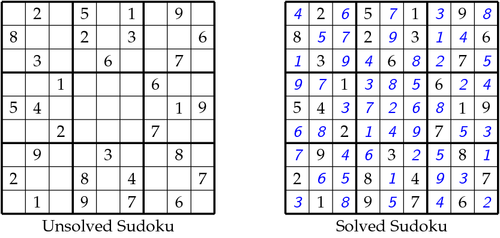
\includegraphics[scale=0.5]{Pendahuluan/Sudoku.png}
\caption[Contoh permainan teka-teki Sudoku dengan solusinya]{Contoh permainan teka-teki Sudoku dengan solusinya}
\label{fig:sudoku}
\end{figure}

Persamaannya, tujuan dari teka-teki ini adalah mengisi setiap sel (\textit{cell}) dalam (\textit{grid}) dengan angka 1 sampai \begin{math}n\end{math} tanpa pengulangan angka dalam setiap kolomnya dan barisnya untuk \textit{grid} berukuran \begin{math}n \times n\end{math}, dengan \begin{math}n\end{math} adalah ukuran \textit{grid}. Tidak ada angka yang boleh muncul lebih dari sekali dalam setiap baris atau kolom dalam \textit{grid}.

Perbedaannya, jika pada Sudoku \textit{grid} berukuran \begin{math}n \times n\end{math} dibagi menjadi \begin{math}n\end{math} (\textit{cage}) dengan setiap \textit{cage} terdiri atas \begin{math}n\end{math} sel, pada Calcudoku \textit{grid} dibagi menjadi sejumlah \textit{cage} yang jumlah selnya bervariasi. Setiap \textit{cage} dibatasi oleh garis yang lebih tebal daripada garis pembatas antar sel. Angka-angka dalam satu \textit{cage} yang sama harus menghasilkan angka tujuan yang telah ditentukan jika dihitung menggunakan operasi matematika yang telah ditentukan (penjumlahan, pengurangan, perkalian, atau pembagian). Angka-angka dalam satu \textit{cage} juga boleh berulang, selama pengulangan tidak terjadi dalam satu kolom atau baris yang sama. Jika \textit{cage} hanya berisi satu sel, maka satu-satunya kemungkinan jawaban untuk sel tersebut adalah angka tujuan dari \textit{cage} tersebut. Angka tujuan dan operasi matematika dituliskan di sudut kiri atas \textit{cage}. Pada awalnya, setiap sel dalam setiap \textit{cage} dalam teka-teki ini kosong, belum terisi oleh angka-angka. \textit{Border line} adalah garis pembatas terluar, \textit{row line} adalah garis pembatas antar baris, dan \textit{column line} adalah garis pembatas antar kolom. Gambar~\ref{fig:hybrid1} menggambarkan contoh sebuah permainan teka-teki Calcudoku ~\cite{fahda:16:backtracking} ~\cite{johanna:12:hybrid}.

\begin{figure}
\centering
\captionsetup{justification=centering}
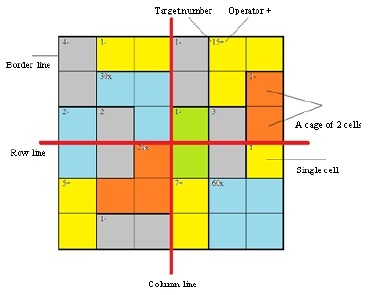
\includegraphics[scale=1]{Gambar/HybridGenetic1}
\caption[Contoh permainan teka-teki Calcudoku dengan penjelasan tentang elemen-elemen dari teka-teki ini ~\cite{johanna:12:hybrid}]{Contoh permainan teka-teki Calcudoku dengan penjelasan elemen-elemen dari teka-teki ini ~\cite{johanna:12:hybrid}}
\label{fig:hybrid1}
\end{figure}

Calcudoku dapat diselesaikan menggunakan beberapa algoritma. Skripsi ini membahas tentang penyelesaian Calcudoku menggunakan algoritma \textit{backtracking} dan algoritma \textit{hybrid genetic}, dan perbandingan performansi \textit{performance} antara kedua algoritma tersebut dalam hal kecepatan dan kesuksesan dalam menyelesaikan Calcudoku.

Algoritma \textit{backtracking} adalah sebuah algoritma umum yang mencari solusi dengan mencoba salah satu dari beberapa pilihan, jika pilihan yang dipilih ternyata salah, komputasi dimulai lagi pada titik pilihan dan mencoba pilihan lainnya. Untuk bisa melacak kembali langkah-langkah yang telah dipilih, maka algoritma harus secara eksplisit menyimpan jejak dari setiap langkah yang sudah pernah dipilih, atau menggunakan rekursi (\textit{recursion}). Rekursi dipilih karena jauh lebih mudah daripada harus menyimpan jejak setiap langkah yang pernah dipilih, hal ini menyebabkan algoritma ini biasanya berbasis DFS (\textit{Depth First Search}) ~\cite{fahda:16:backtracking}.

Algoritma \textit{rule based} adalah sebuah algoritma berbasis aturan logika untuk menyelesaikan permainan teka-teki Sudoku dan variasinya, termasuk Calcudoku. Beberapa aturan logika yang digunakan dalam algoritma ini adalah \textit{single square rule}, \textit{naked subset rule}, \textit{hidden single rule}, \textit{evil twin rule}, \textit{killer combination}, dan \textit{X-wing}.

Pencarian heuristik adalah sebuah teknik pencarian kecerdasan buatan (\textit{artifical intelligence}) yang menggunakan heuristik dalam langkah-langkahnya. Heuristik adalah semacam aturan tidak tertulis yang mungkin menghasilkan solusi. Heuristik kadang-kadang efektif, tetapi tidak dijamin akan berhasil. dalam setiap kasus. Heuristik memerankan peran penting dalam strategi pencarian karena sifat eksponensial dari kebanyakan masalah. Heuristik membantu mengurangi jumlah alternatif solusi dari angka yang bersifat eksponensial menjadi angka yang bersifat polinomial. Contoh teknik pencarian heuristik adalah \textit{Generate and Test}, \textit{Hill Climbing}, dan \textit{Best First Search}.

Algoritma genetik adalah salah satu teknik heuristik \textit{Generate and Test} yang terinspirasi oleh sistem seleksi alam. Algoritma ini adalah perpaduan dari bidang biologi dan ilmu komputer. Algoritma ini adalah salah satu dari teknik pencarian heuristik.

Algoritma ini memanipulasi informasi, biasanya disebut sebagai kromosom. Kromosom ini mengkodekan kemungkinan jawaban untuk sebuah masalah yang diberikan. Kromosom dievaluasi dan diberi \textit{fitness value} berdasarkan seberapa baikkah kromosom dalam menyelesaikan maslah yang diberikan berdasarkan kriteria yang ditentukan oleh pembuat program. Nilai kelayakan ini digunakan sebagai probabilitas kebertahanan hidup kromosom dalam satu siklus reproduksi. Kromosom baru (kromosom anak, \textit{child chromosome}) diproduksi dengan menggabungkan dua (atau lebih) kromosom orang tua (\textit{parent chromosome}). Proses ini dirancang untuk menghasilkan kromosom-kromosom keturunan yang lebih layak, kromosom-kromosom ini menyandikan jawaban yang lebih baik, sampai solusi yang baik dan yang bisa diterima ditemukan.

Algoritma \textit{hybrid genetic} adalah gabungan antara algoritma genetik dan algoritma-algoritma lainnya. Dalam kasus ini, algoritma genetik digabungkan dengan algoritma \textit{rule based}. Algoritma \textit{rule based} akan dijalankan sampai pada titik dimana algoritma tidak bisa menyelesaikan permainan teka-teki Calcudoku. Jika algoritma sudah tidak bisa menyelesaikan permainan, maka algoritma genetik akan mulai dijalankan ~\cite{johanna:12:hybrid}.

\section{Rumusan Masalah}
\label{sec:rumusan}
Berdasarkan latar belakang yang telah diuraikan di atas, dapat dirumuskan permasalahan sebagai berikut:
\begin{enumerate}
\item Bagaimana cara mengimplementasikan perangkat lunak (\textit{software}) permainan teka-teki Calcudoku?
\item Bagaimana cara mengimplementasikan algoritma \textit{backtracking} untuk menyelesaikan Calcudoku?
\item Bagaimana cara mengimplementasikan algoritma \textit{hybrid genetic} untuk menyelesaikan Calcudoku?
\item Bagaimana perbandingan performansi algoritma \textit{backtracking} dengan algoritma \textit{hybrid genetic} dalam menyelesaikan Calcudoku?
\end{enumerate}

\section{Tujuan}
\label{sec:tujuan}
Berdasarkan rumusan masalah yang telah dirumuskan, maka tujuan dari pembuatan skripsi ini adalah:
\begin{enumerate}
\item Membuat perangkat lunak permainan teka-teki Calcudoku yang menerima input berupa soal teka-teki dan mampu menyelesaikan soal teka-teki tersebut menggunakan algoritma \textit{backtracking} dan \textit{hybrid genetic}.
\item Membandingkan performansi algoritma \textit{backtracking} dengan algoritma \textit{hybrid genetic} dalam hal kecepatan dan kesuksesan dalam menyelesaikan Calcudoku.
\end{enumerate}

\section{Batasan Masalah}
\label{sec:batasan}
Ruang lingkup dari skripsi ini dibatasi oleh batasan-batasan masalah sebagai berikut:
\begin{enumerate}
\item Ukuran \textit{grid} untuk permainan teka-teki Calcudoku adalah antara \begin{math}3 \times 3\end{math} sampai dengan \begin{math}8 \times 8\end{math}. Pada awalnya, ukuran \textit{grid} direncanakan akan dibatasi sampai dengan \begin{math}9 \times 9\end{math}, tetapi karena ada masalah saat pengujian (keluar pesan error "\textit{Memory full}" saat menguji \textit{solver} dengan algoritma \textit{backtracking} pada \textit{grid} yang berukuran \begin{math}9 \times 9\end{math}, maka ukuran \textit{grid} dibatasi sampai dengan \begin{math}8 \times 8\end{math}.
\item Pada algoritma \textit{rule based}, yang merupakan bagian dari algoritma \textit{hybrid genetic}, aturan-aturan logika yang digunakan dibatasi hanya pada aturan \textit{single square}, \textit{naked single}, \textit{naked double}, \textit{hidden single}, \textit{killer combination}, dan \textit{evil twin}.
\end{enumerate}

\section{Metodologi Penelitian}
\label{sec:metlit}
Langkah-langkah yang akan dilakukan dalam pembuatan skripsi ini adalah:
\begin{enumerate}
\item Studi literatur
\begin{enumerate}
\item Melakukan studi literatur tentang permainan teka-teki Calcudoku.
\item Melakukan studi literatur tentang algoritma \textit{backtracking}.
\item Melakukan studi literatur tentang algoritma \textit{rule based} dan algoritma genetik.
\end{enumerate}
\item Analisis, perancangan, dan pengembangan perangkat lunak
\begin{enumerate}
\item Melakukan analisis dan menentukan fitur-fitur yang diperlukan dalam perangkat lunak permainan teka-teki Calcudoku.
\item Membuat perangkat lunak Calcudoku dengan fitur-fitur yang telah ditentukan. 
\item Mengimplementasikan algoritma \textit{backtracking} untuk Calcudoku.
\item Mengimplementasikan algoritma \textit{hybrid genetic} untuk Calcudoku.
\item Membandingkan performansi algoritma \textit{backtracking} dengan algoritma \textit{hybrid genetic} dalam menyelesaikan Calcudoku.
\end{enumerate}
\item Melakukan pengujian dan eksperimen terhadap perangkat lunak Calcudoku yang telah dibuat.
\item Membuat kesimpulan berdasarkan hasil pengujian perangkat lunak yang telah dibuat.
\end{enumerate}

\section{Sistematika Pembahasan}
\label{sec:sispem}
Sistematika pembahasan skripsi ini adalah sebagai berikut:
\begin{enumerate}
\item Bab 1 berisi latar belakang, rumusan masalah, tujuan, batasan masalah, metodologi penelitian, dan sistematika pembahasan dari skripsi ini.
\item Bab 2 membahas tentang landasan teori yang digunakan dalam skripsi ini, yaitu tentang permainan teka-teki Calcudoku, algoritma \textit{backtracking} dan algoritma \textit{hybrid genetic}.
\item Bab 3 membahas tentang analisis perangkat lunak Calcudoku dan analisis algoritma \textit{backtracking} dan algoritma \textit{hybrid genetic}.
\item Bab 4 membahas tentang perancangan dan pembuatan perangkat lunak Calcudoku dan algoritma \textit{backtracking} dan algoritma \textit{hybrid genetic} untuk menyelesaikan permainan, perancangan antarmuka (\textit{interface}), input dan output, diagram kelas (\textit{class diagram}), dan diagram aktivitas (\textit{activity diagram}).
\item Bab 5 membahas tentang implementasi dari perangkat lunak Calcudoku dan algoritma \textit{backtracking} dan algoritma \textit{hybrid genetic} yang telah dirancang, implementasi antarmuka, input dan output yang telah dirancang, dan pengujian perangkat lunak Calcudoku dalam hal perbandingan performansi algoritma \textit{backtracking} dan algoritma \textit{hybrid genetic} dalam menyelesaikan permainan.
\item Bab 6 berisi kesimpulan dari pembuatan perangkat lunak Calcudoku dan hasil pengujiannya, dan saran untuk penelitian pengembangan perangkat lunak selanjutnya.
\end{enumerate}}{}  
\ifdefstring{\vbabb}{1}{\chapter{Landasan Teori}
\label{chap:teori}

Bab ini membahas tentang landasan teori yang akan digunakan dalam skripsi ini yang diambil dari dua sumber, yaitu ''KenKen Puzzle Solver using Backtracking Algorithm'' karya Asanilta Fahda ~\cite{fahda:16:backtracking} dan ''Solving and Modeling Ken-ken Puzzle by Using Hybrid Genetics Algorithm'' karya Olivia Johanna, Samuel Lukas, dan Kie Van Ivanky Saputra ~\cite{johanna:12:hybrid}.

\section{Calcudoku ~\cite{fahda:16:backtracking} ~\cite{johanna:12:hybrid}}
\label{sec:calcudoku}
Sebagai salah satu jenis permainan teka-teki aritmatika dan \textit{grid}, Calcudoku, atau dikenal juga sebagai KenKen, KenDoku, atau Mathdoku, diciptakan pada tahun 2004 oleh seorang guru matematika dari Jepang yang bernama Tetsuya Miyamoto untuk memenuhi tujuannya untuk melatih kemampuan matematika dan logika siswa-siswinya dengan cara yang menyenangkan. Nama KenKen diambil dari kata bahasa Jepang yang berarti kepandaian. Permainan yang mengasah otak ini dengan cepat menyebar ke seluruh Jepang dan Amerika Serikat, menggantikan permainan teka-teki silang di banyak koran. Permainan ini kemudian menjadi sensasi di seluruh dunia setelah munculnya versi \textit{online} dan \textit{mobile} dari permainan teka-teki ini, khususnya menarik untuk pecinta permainan teka-teki angka seperti Sudoku.

Seperti dalam Sudoku, dalam teka-teki ini, pemain diberikan sebuah \textit{grid} dengan ukuran \begin{math}n \times n\end{math}, dengan \begin{math}n\end{math} biasanya \begin{math}3 \leq n \leq 9\end{math}. \textit{Grid} ini harus diisi dengan angka 1 sampai dengan \begin{math}n\end{math} sehingga dalam setiap baris setiap angka hanya muncul sekali, dalam setiap kolom setiap angka hanya muncul sekali. Perbedaannya dengan Sudoku adalah, Calcudoku dibagi ke dalam \textit{cage} (sekelompok sel yang dibatasi oleh garis yang lebih tebal daripada garis pembatas antar sel, setiap \textit{cage} mempunyai angka tujuan dan operator yang telah ditentukan), dan angka-angka dalam setiap \textit{cage} harus mencapai angka tujuan jika dihitung menggunakan operator yang telah ditentukan. Angka tujuan dan operasi yang telah ditentukan ditulis di sudut kiri atas \textit{cage}. Ada lima kemungkinan operator:
\begin{enumerate}
\item +, sebuah operator \begin{math}n\end{math}-ary yang menandakan penjumlahan.
\item -, sebuah operator biner yang menandakan pengurangan.
\item \begin{math}\times\end{math}, sebuah operator \begin{math}n\end{math}-ary yang menandakan perkalian.
\item \begin{math}\div\end{math} sebuah operator biner yang menandakan pembagian.
\item =, (simbol ini biasanya dihilangkan), sebuah operator uner yang menandakan persamaan.
\end{enumerate}
Jika operasi matematika yang ditentukan adalah pengurangan atau pembagian, maka ukuran \textit{cage} harus berukuran dua sel. Pada beberapa versi dari teka-teki ini, hanya angka tujuan yang diberikan, dan pemain harus menebak operator dari setiap \textit{cage} untuk menyelesaikan teka-tekinya ~\cite{fahda:16:backtracking} ~\cite{johanna:12:hybrid}.

\begin{figure}
\centering
\captionsetup{justification=centering}
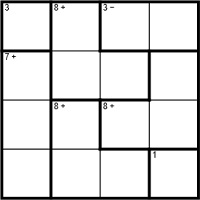
\includegraphics[scale=0.75]{Gambar/Backtracking1}
\caption[Contoh permainan teka-teki Calcudoku dengan ukuran \textit{grid} 4 x 4 yang belum diselesaikan. ~\cite{fahda:16:backtracking}]{Contoh permainan teka-teki dengan ukuran \textit{grid} 4 x 4 yang belum diselesaikan. ~\cite{fahda:16:backtracking}}
\label{fig:backtracking1}
\end{figure}

Untuk menyelesaikan sebuah teka-teki Calcudoku, pemain pertama-tama harus memahami dua permasalahan utama dari teka-teki ini, yaitu:
\begin{enumerate}
\item Angka-angka mana yang harus dimasukkan ke dalam sebuah \textit{cage}
\item Dalam urutan apa angka-angka tersebut harus dimasukkan ke dalam sebuah \textit{cage}
\end{enumerate}

Seperti kebanyakan permainan teka-teki angka, cara yang paling mudah untuk menyelesaikan teka-teki ini adalah dengan mengeliminasi angka-angka yang sudah digunakan dan mencoba satu per satu angka yang mungkin (\textit{trial and error}). 

Dalam pengisian teka-teki ini ada dua tahapan, yaitu:
\begin{enumerate} 
\item Mencari \textit{cage} yang hanya berukuran 1 sel, karena \textit{cage} ini tidak menghasilkan pertanyaan angka apa dan urutan apa. Tahap ini adalah tahap yang paling jelas. Contoh, pada Gambar~\ref{fig:backtracking1}, \textit{cage} pada sudut kiri atas dan \textit{cage} pada sudut kanan bawah hanya berukuran 1 sel, dan dapat langsung diisi dengan angka tujuannya.
\item Mencari \textit{cage} yang hanya mempunyai satu kemungkinan kombinasi angka, sehingga masalah angka-angka apa yang harus diisi dalam \textit{cage} tersebut terjawab. Contoh, \textit{cage} pada sudut kanan atas mempunyai aturan "3-", artinya angka tujuannya adalah 3 dengan menggunakan operasi pengurangan. Satu-satunya pasangan angka dari himpunan \{1,2,3,4\} yang akan menghasilkan angka 3 saat satu angka dikurangkan dari angka yang lainnya adalah \{1,4\}. Namun masalahnya adalah urutan angka-angka yang harus dimasukkan. Dalam kasus ini, untungnya, sel pada sudut kanan bawah sudah diisi dengan angka 1, maka angka 1 tidak bisa digunakan lagi pada kolom yang paling kanan. Jadi, dengan menggunakan cara eliminasi, sel pada sudut kanan atas harus diisi dengan angka 4 dan sel di sebelah kirinya, yaitu sel pada baris yang paling atas dan kolom ketiga dari kiri, harus diisi dengan angka 1. Hal ini memberikan solusi untuk sel pada baris yang paling atas dan kolom kedua dari kiri, yaitu angka 2, karena angka 2 adalah angka yang belum pernah dipakai dalam baris tersebut. Proses ini berlanjut sampai semua sel dalam \textit{grid} terisi dan menghasilkan solusi pada Gambar~\ref{fig:backtracking2} ~\cite{fahda:16:backtracking}.
\end{enumerate}

\begin{figure}
\centering
\captionsetup{justification=centering}
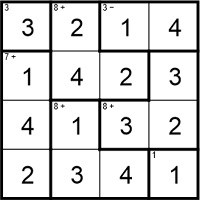
\includegraphics[scale=0.75]{Gambar/Backtracking2}
\caption[Solusi untuk permainan teka-teki Calcudoku yang diberikan pada Gambar~\ref{fig:backtracking1} ~\cite{fahda:16:backtracking}]{Solusi untuk permainan teka-teki Calcudoku yang diberikan pada Gambar~\ref{fig:backtracking1}.}
\label{fig:backtracking2}
\end{figure}

Seiring dengan meningkatnya tingkat kesulitan, langkah berikutnya tidak akan langsung muncul dengan jelas. Kadang-kadang, pemain mencapai titik dimana langkah berikutnya tidak pasti. Pemain harus menebak langkah-langkah berikutnya dan melihat apakah langkah ini akan menghasilkan solusinya. Jika tidak, pemain harus mundur kembali ke titik ketidakpastian tersebut.

Sebuah teka-teki Calcudoku dengan ukuran \begin{math}n \times n\end{math}, dengan \begin{math}n\end{math} melambangkan jumlah sel dalam satu baris atau kolom, mempunyai \begin{math}n^2\end{math} sel dalam sebuah \textit{grid}. Sel yang terletak dalam baris \begin{math}b\end{math} dan kolom \begin{math}k\end{math} diberi label \begin{math}C_{b,k} = bn + k\end{math} dan nilai dari sel tersebut adalah \begin{math}V(C_{b,k}) \in \{1, 2, ..., n\}\end{math}. Nomor baris \begin{math}b\end{math} memiliki \textit{range} \begin{math}0 \leq b \leq n - 1\end{math}. Nomor kolom \begin{math}k\end{math} memiliki \textit{range} \begin{math}0 \leq k \leq n - 1\end{math}. Nomor sel \begin{math}C\end{math} memiliki \textit{range} \begin{math}0 \leq C \leq n^2 - 1\end{math}. Nomor sel adalah hasil perkalian dari nomor baris tempat sebuah sel berada dikalikan dengan banyaknya sel dalam sebuah baris, lalu dijumlahkan dengan nomor kolom tempat sebuah sel berada. Sebuah \textit{cage}, yang diberi label \begin{math}A_i\end{math} adalah sebuah himpunan dari sel, yaitu \begin{math}A_i = \{C_{b,k}\}\end{math}. Setiap \textit{cage} terhubung dengan satu operator aritmatika \begin{math}O_i \in \{+, -, \times, \div, =\}\end{math}, artinya operator aritmatika adalah salah satu dari penjumlahan, pengurangan, perkalian, pembagian, dan sama dengan, dan satu angka tujuan \begin{math}H_i \in N\end{math}, artinya angka tujuan adalah sebuah bilangan asli. Tiga aturan dalam mendefinisikan masalah dalam Calcudoku adalah sebagai berikut ~\cite{johanna:12:hybrid}:
\begin{enumerate}
\item \begin{math}|A_i| = 1 \rightarrow O_i = \phi\end{math}, artinya setiap \textit{cage} yang jumlah selnya 1 dengan operasi matematika yang terkait dengan \textit{cage} tersebut memiliki hubungan korespondensi satu ke satu.
\item \begin{math}O_i \in \{-, \div\} \rightarrow |A_i| = 2\end{math}, artinya jika operasi yang digunakan dalam sebuah \textit{cage} adalah pengurangan atau pembagian, maka jumlah sel dalam \textit{cage} tersebut harus 2.
\item \begin{math}\forall C_{b,k} \rightarrow C_{b,k} \in \exists! A_i\end{math}, artinya setiap sel hanya boleh menjadi anggota dari satu dan hanya satu \textit{cage}.
\end{enumerate}
Tujuan dari teka-teki ini adalah untuk mencari nilai \begin{math}V(C_{b,k})\end{math} dan memenuhi persyaratan berikut ~\cite{johanna:12:hybrid}:
\begin{enumerate}
\item \begin{math}|A_i| = 1 \land C_{b,k} \in A_i \rightarrow V(C_{b,k}) = H_i\end{math}, artinya jika sel adalah bagian dari sebuah \textit{cage} yang jumlah selnya 1, maka nilai dari sel tersebut adalah angka tujuan dari \textit{cage} tersebut.
\item \begin{math}O_i \in \{-\} \land A_i = \{C_{a,b}, C_{p,q}\} \rightarrow |V(C_{a,b}) - V(C_{p,q})| = H_i\end{math}, artinya jika sebuah \textit{cage} yang operasi matematikanya adalah pengurangan, maka nilai absolut dari hasil pengurangan nilai kedua sel di dalam \textit{cage} tersebut adalah angka tujuan dari \textit{cage} tersebut.
\item \begin{math}O_i \in \{\div\} \land A_i = \{C_{a,b}, C_{p,q}\} \rightarrow V(C_a,_b) / V(C_{p,q}) = H_i\end{math}, artinya jika sebuah \textit{cage} yang operasi matematikanya adalah pembagian, maka nilai dari hasil pembagian nilai kedua sel di dalam \textit{cage} tersebut adalah angka tujuan dari \textit{cage} tersebut.
\item \begin{math}O_i \in \{+\} \rightarrow \sum_{C_{b,k} \in A_i} V(C_{b,k}) = H_i\end{math}, artinya jika sebuah \textit{cage} yang operasi matematikanya adalah penjumlahan, maka nilai dari hasil penjumlahan dari nilai semua sel di dalam \textit{cage} tersebut adalah angka tujuan dari \textit{cage} tersebut.
\item \begin{math}O_i \in \{\times\} \rightarrow \prod_{C_{b,k} \in A_i} V(C_{b,k}) = H_i\end{math}, artinya jika sebuah \textit{cage} yang operasi matematikanya adalah perkalian, maka nilai dari hasil perkalian dari nilai semua sel di dalam \textit{cage} tersebut adalah angka tujuan dari \textit{cage} tersebut.
\end{enumerate}

\section{Algoritma \textit{Backtracking} ~\cite{fahda:16:backtracking}}
\label{sec:backtracking}

Algoritma \textit{backtracking} adalah sebuah algoritma umum yang mencari solusi dengan mencoba salah satu dari beberapa pilihan, jika pilihan yang dipilih ternyata salah, komputasi dimulai lagi pada titik pilihan dan mencoba pilihan lainnya. Untuk bisa melacak kembali langkah-langkah yang telah dipilih, maka algoritma harus secara eksplisit menyimpan jejak dari setiap langkah yang sudah pernah dipilih, atau menggunakan rekursi (\textit{recursion}). Rekursi dipilih karena jauh lebih mudah daripada harus menyimpan jejak setiap langkah yang pernah dipilih. Hal ini menyebabkan algoritma ini biasanya berbasis DFS (\textit{Depth First Search}).

Algoritma \textit{backtracking} pertama kali diperkenalkan pada tahun 1950 oleh D.H. Lehmer sebagai perbaikan algoritma \textit{brute force}. Algoritma ini lalu dikembangkan lebih lanjut oleh R.J. Walker, S.W. Golomb, dan L.D. Baumert. Algoritma ini terbukti efektif untuk menyelesaikan banyak permainan logika (misalnya \textit{tic tac toe}, \textit{maze}, catur, dan lain-lain) karena algoritma itu terutama berguna untuk menyelesaikan masalah-masalah \textit{constraint satisfaction}, di mana sekumpulan objek harus memenuhi sejumlah batasan.

Implementasi algoritma \textit{backtracking} memiliki tiga sifat umum, yaitu ~\cite{fahda:16:backtracking}:
\begin{enumerate}
\item \textit{Solution space}
\\ Solusi untuk masalah ini dinyatakan sebagai sebuah vektor \begin{math}X\end{math} dengan \textit{\begin{math}n\end{math}-tuple}:
\begin{displaymath}
X = (x_1, x_2, ..., x_n), x_i \in S_i
\end{displaymath}
di mana adalah mungkin bahwa:
\begin{displaymath}
S_1 = S_2 = ... = S_n
\end{displaymath} 
\item Fungsi pembangkit \begin{math}X_k\end{math} (\textit{generating function})
\\ Fungsi pembangkit \begin{math}X_k\end{math} dinyatakan sebagai:
\begin{displaymath}
T(k)
\end{displaymath}
di mana \begin{math}T(k)\end{math} membangkitkan nilai \begin{math}X_k\end{math}, dari 1 sampai \begin{math}n\end{math}, yang merupakan komponen dari vektor solusi.
\item Fungsi pembatas (\textit{bounding function})
\\ Fungsi pembatas dinyatakan sebagai:
\begin{displaymath}
B(x_1, x_2, ..., x_k)
\end{displaymath}
di mana B bernilai \textit{true} jika \begin{math}(x_1, x_2, ..., x_k)\end{math} mengarah ke solusi. Jika B bernilai \textit{true}, maka nilai \begin{math}x_k+1\end{math} akan terus dibangkitkan, dan jika B bernilai \textit{false}, maka \begin{math}(x_1, x_2, ..., x_k)\end{math} akan dibuang.
\end{enumerate}

Ruang solusi untuk algoritma \textit{backtracking} disusun dalam sebuah struktur berbentuk pohon (\textit{tree}), di mana setiap simpul (\textit{node}) merepresentasikan keadaan masalah dan sisi (\textit{edge}) diberi label \begin{math}x_i\end{math}. Jalur dari akar (\textit{root}) ke daun (\textit{leaf}) merepresentasikan sebuah jawaban yang mungkin, dan semua jalur yang dikumpulkan bersama-sama membentuk ruang solusi. Struktur pohon ini disebut sebagai \textit{state space tree}. Gambar~\ref{fig:backtracking3} menggambarkan contoh sebuah \textit{state space tree}.

\begin{figure}
\centering
\captionsetup{justification=centering}
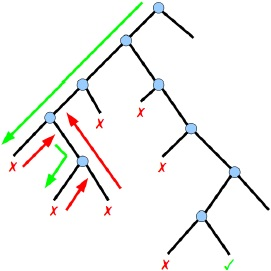
\includegraphics[scale=1]{Gambar/Backtracking3}
\caption[Ilustrasi \textit{State space tree} yang digunakan dalam algoritma \textit{backtracking} ~\cite{fahda:16:backtracking}]{Ilustrasi \textit{State space tree} yang digunakan dalam algoritma \textit{backtracking} ~\cite{fahda:16:backtracking}}
\label{fig:backtracking3}
\end{figure}

Langkah-langkah dalam menggunakan \textit{state space tree} untuk mencari solusi adalah ~\cite{fahda:16:backtracking}:
\begin{enumerate}
\item Solusi dicari dengan membangun jalur dari akar ke daun menggunakan algoritma DFS.
\item Simpul yang terbentuk disebut sebagai simpul hidup (\textit{live nodes}).
\item Simpul yang sedang diperluas disebut sebagai \textit{expand nodes} atau \textit{E-nodes}.
\item Setiap kali sebuah \textit{E-node} sedang diperluas, jalur yang dikembangkannya menjadi lebih panjang.
\item Jika jalur yang sedang dikembangkan tidak mengarah ke solusi, maka \textit{E-node} dimatikan dan menjadi simpul mati (\textit{dead node}).
\item Fungsi yang digunakan untuk mematikan \textit{E-node} adalah implementasi dari fungsi pembatas.
\item Simpul mati tidak akan diperluas.
\item Jika jalur yang sedang dibangun berakhir dengan simpul mati, proses akan mundur ke simpul sebelumnya.
\item Simpul sebelumnya terus membangkitkan simpul anak (\textit{child node}) lainnya, yang kemudian menjadi \textit{E-node} baru.
\item Pencarian selesai jika simpul tujuan tercapai.
\end{enumerate}
Setiap simpul di dalam \textit{state space tree} terkait dengan panggilan rekursif. Jika jumlah simpul di dalam pohon \begin{math}2n\end{math} atau \begin{math}n!\end{math}, maka pada kasus terburuk untuk algoritma \textit{backtracking} ini memiliki kompleksitas waktu \begin{math}O(p(n)2n)\end{math} atau \begin{math}O(q(n)n!)\end{math}, dengan \begin{math}p(n)\end{math} dan \begin{math}q(n)\end{math} sebagai polinomial dengan \begin{math}n\end{math}-derajat menyatakan waktu komputasi untuk setiap simpul.

Ruang solusi untuk sebuah permainan teka-teki Calcudoku dengan \textit{grid} yang berukuran \begin{math}n \times n\end{math} adalah \begin{math}X = (x_1,x_2,...,x_m), x_i \in \{1,2,...,n\}\end{math}, dengan \begin{math}m = n^2\end{math}. Jadi, \begin{math}n\end{math} adalah jumlah sel dalam satu baris atau kolom, \begin{math}X\end{math} adalah sebuah himpunan yang merepresentasikan isi dari setiap sel dalam \textit{grid}, dimulai pada sel pada sudut kiri atas, lalu bergerak ke sel di sebelah kanannya dalam baris yang sama, jika sudah mencapai sel yang paling kanan maka bergerak ke sel yang paling kiri pada baris dibawahnya, hingga berakhir pada sel pada sudut kanan bawah, dan \begin{math}S_i\end{math} adalah sebuah himpunan yang berisi angka-angka dari 1 sampai \begin{math}n\end{math}.

Fungsi pembangkit membangkitkan sebuah integer secara berurutan dari 1 sampai \begin{math}n\end{math} sebagai \begin{math}x_k\end{math}. Fungsi pembatas menggabungkan tiga fungsi pemeriksa pembatas (\textit{constraint checking}), yaitu fungsi pemeriksa kolom (\textit{column checking}), fungsi pemeriksa baris (\textit{row checking}), dan fungsi pemeriksa \textit{grid} (\textit{grid checking}).

Fungsi pemeriksa kolom menghasilkan nilai \textit{true} jika \begin{math}x_k\end{math} belum ada di dalam kolom dan menghasilkan nilai \textit{false} jika \begin{math}x_k\end{math} sudah ada di dalam kolom.

Fungsi pemeriksa baris menghasilkan nilai \textit{true} jika \begin{math}x_k\end{math} belum ada di dalam baris dan menghasilkan nilai \textit{false} jika \begin{math}x_k\end{math} sudah ada di dalam baris.

Fungsi pemeriksa \textit{grid} memeriksa operator pada \textit{grid} dan memeriksa berdasarkan operator yang telah ditentukan. Ada 5 operator yang digunakan dalam fungsi ini, yaitu:

\begin{enumerate}
\item Operator penjumlahan (+), fungsi menghasilkan nilai \textit{true} jika hasil penjumlahan semua nilai yang ada pada \textit{grid} ditambah dengan \begin{math}x_k\end{math} kurang dari atau sama dengan nilai tujuan, dan menghasilkan nilai \textit{false} jika jumlah semua nilai yang ada pada \textit{grid} ditambah \begin{math}x_k\end{math} lebih dari nilai tujuan.
\item Operator pengurangan (-), fungsi menghasilkan nilai \textit{true} jika kedua sel dalam \textit{grid} kosong, atau jika ada satu sel yang kosong dan hasil dari \begin{math}x_k\end{math} dikurangi dengan nilai dari sel yang lainnya atau hasil dari nilai dari sel yang lainnya dikurangi dengan \begin{math}x_k\end{math} menghasilkan nilai tujuan, dan menghasilkan nilai \textit{false} jika ada satu sel kosong dan hasil dari \begin{math}x_k\end{math} dikurangi dengan nilai dari sel yang lainnya atau hasil dari nilai dari sel yang lainnya dikurangi dengan \begin{math}x_k\end{math} tidak menghasilkan nilai tujuan.
\item Operator perkalian (\begin{math}\times\end{math}), fungsi menghasilkan nilai \textit{true} jika hasil perkalian dari semua nilai yang ada pada \textit{grid} dikali dengan \begin{math}x_k\end{math} kurang dari atau sama dengan nilai tujuan, dan menghasilkan nilai \textit{false} jika hasil perkalian dari semua nilai yang ada pada \textit{grid} dikali dengan \begin{math}x_k\end{math} lebih dari nilai tujuan.
\item Operator pembagian (\begin{math}\div\end{math}), fungsi menghasilkan nilai \textit{true} jika kedua sel dalam \textit{grid} kosong, atau jika ada satu sel yang kosong dan hasil dari \begin{math}x_k\end{math} dibagi dengan nilai dari sel yang lainnya atau hasil dari nilai dari sel yang lainnya dibagi dengan \begin{math}x_k\end{math} menghasilkan nilai tujuan, dan menghasilkan nilai \textit{false} jika ada satu sel yang kosong dan hasil dari \begin{math}x_k\end{math} dibagi dengan nilai dari sel yang lainnya atau hasil dari nilai dari sel yang lainnya dibagi dengan \begin{math}x_k\end{math} tidak menghasilkan nilai tujuan.
\item Operator =, fungsi akan menghasilkan nilai \textit{true} jika \begin{math}x_k\end{math} sama dengan nilai tujuan, dan menghasilkan nilai \textit{false} jika \begin{math}x_k\end{math} tidak sama dengan nilai tujuan.
\end{enumerate}

\textit{State space tree} bersifat dinamis, berkembang secara terus-menerus sampai solusi ditemukan. Untuk mengilustrasikan berkembangnya \textit{state space tree}, teka-teki Calcudoku yang digambarkan pada Gambar~\ref{fig:backtracking4} akan digunakan. Berikut ini adalah tahap-tahap berkembangnya \textit{state space tree} untuk teka-teki tersebut.

\begin{figure}
\centering
\captionsetup{justification=centering}
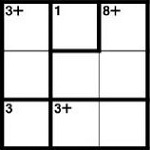
\includegraphics[scale=0.75]{Gambar/Backtracking4}
\caption[Contoh permainan teka-teki Calcudoku dengan ukuran \textit{grid} 3 x 3 ~\cite{fahda:16:backtracking}]{Contoh permainan teka-teki Calcudoku dengan ukuran \textit{grid} 3 x 3 ~\cite{fahda:16:backtracking}}
\label{fig:backtracking4}
\end{figure}

\begin{enumerate}
\item \textit{State space tree} dimulai dengan \textit{state} 1 yang merepresentasikan sebuah \textit{grid} yang kosong.
\item Fungsi pembangkit pertama-tama akan membangkitkan angka 1 sebagai \begin{math}x_1\end{math}, yang akan diisikan pada sel pertama yang kosong, yaitu sel yang terletak di sudut kiri atas \textit{grid}, atau sel pada kolom ke-1 dan baris ke-1 (\textit{state} 2). Fungsi pembatas akan memeriksa jika langkah ini adalah langkah yang berlaku, dan ternyata langkah ini berlaku.
\item Untuk sel yang kosong berikutnya, yaitu \begin{math}x_2\end{math}, atau sel pada kolom ke-2 dan baris ke-1, fungsi pembangkit akan membangkitkan angka 1 (\textit{state} 3), tetapi langkah ini gagal dalam pemeriksaan baris dalam fungsi pembatas karena angka 1 sudah pernah digunakan pada baris tersebut, ini membentuk sebuah simpul mati.
\item Fungsi pembangkit akan mencoba kemungkinan angka berikutnya, yaitu angka 2 (\textit{state} 4), tetapi langkah ini gagal dalam pemeriksaan \textit{grid} dalam fungsi pembatas karena angka 2 tidak sama dengan angka tujuan, yaitu angka 1.
\item Fungsi pembangkit akan mencoba kemungkinan angka berikutnya, yaitu angka 3 (\textit{state} 5), tetapi langkah ini juga gagal dalam pemeriksaan \textit{grid} dalam fungsi pembatas karena angka 3 tidak sama dengan angka tujuan, yaitu angka 1. Gambar~\ref{fig:backtracking5} menggambarkan \textit{state} 3, \textit{state} 4, dan \textit{state} 5 dalam penyelesaian teka-teki Calcudoku ini.

\begin{figure}
\centering
\captionsetup{justification=centering}
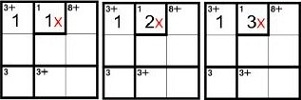
\includegraphics[scale=1]{Gambar/Backtracking5}
\caption[Ilustrasi \textit{state} 3, 4, dan 5 pada sebuah \textit{grid} teka-teki Calcudoku ~\cite{fahda:16:backtracking}]{Ilustrasi \textit{state} 3, 4, dan 5 pada sebuah \textit{grid} teka-teki Calcudoku ~\cite{fahda:16:backtracking}}
\label{fig:backtracking5}
\end{figure}

\item Karena tidak ada solusi yang mungkin, maka mundur ke \textit{state} 1. Fungsi pembangkit akan membangkitkan kemungkinan angka berikutnya sebagai \begin{math}x_1\end{math}, yaitu 2, dan ternyata angka 2 berlaku sebagai \begin{math}x_1\end{math} (\textit{state} 6), sehingga bisa maju ke \begin{math}x_2\end{math}, yaitu sel pada kolom ke-2 dan baris ke-1.
\item Fungsi pembangkit akan membangkitkan angka 1 (\textit{state} 7), dan ini memenuhi syarat yang ditentukan dalam fungsi pembatas, karena angka 1 sama dengan angka tujuan, yaitu angka 1, sehingga bisa maju ke \begin{math}x_3\end{math}, yaitu sel pada kolom ke-3 dan baris ke-1.
\item Angka 1 (\textit{state} 8) gagal dalam pemeriksaan baris karena angka 1 sudah pernah digunakan pada baris tersebut.
\item Angka 2 (\textit{state} 9) juga gagal dalam pemeriksaan baris karena angka 2 sudah pernah digunakan pada baris tersebut.
\item Hal ini menyebabkan hanya tersisa angka 3 sebagai angka yang bisa dimasukkan ke dalam \begin{math}x_3\end{math} (\textit{state} 10). Karena \textit{state} 10 ternyata berlaku, baris ke-1 telah selesai diisi, dan bisa maju ke baris ke-2.
\item Langkah berikutnya adalah membuat \textit{state} baru dengan mengisikan angka 1 pada \begin{math}x_4\end{math}, yaitu sel pada kolom ke-1 dan baris ke-2 (\textit{state} 11). Ini memenuhi pemeriksaan pembatas, karena 2 + 1 = 3, sehingga akan maju ke sel berikutnya, yaitu \begin{math}x_5\end{math}, atau sel pada kolom ke-2 dan baris ke-2.
\item Angka 1 (\textit{state} 12) jelas tidak bisa digunakan karena gagal dalam pemeriksaan kolom dan pemeriksaan baris; angka 1 sudah pernah digunakan pada kolom dan baris tersebut.
\item Angka 2 (\textit{state} 13) adalah langkah yang berlaku, sehingga bisa maju ke sel berikutnya, yaitu \begin{math}x_6\end{math}, atau sel pada kolom ke-3 dan baris ke-2.
\item Langkah berikutnya adalah mengisikan \begin{math}x_6\end{math} dengan angka 1 (\textit{state} 14), tetapi gagal dalam pemeriksaan baris karena angka 1 sudah pernah digunakan pada baris tersebut.
\item Langkah berikutnya adalah mencoba kemungkinan angka berikutnya, yaitu angka 2 (\textit{state} 15), tetapi juga gagal dalam pemeriksaan baris karena angka 2 sudah pernah digunakan pada baris tersebut.
\item Langkah berikutnya adalah mencoba kemungkinan angka berikutnya, yaitu angka 3 (\textit{state} 16), tetapi juga gagal, kali ini angka 3 gagal dalam pemeriksaan kolom karena angka 3 sudah pernah digunakan pada kolom tersebut.
\item Karena semua kemungkinan angka gagal dalam pemeriksaan baris dan kolom, maka akan mundur ke \textit{state} 11 dan mencoba kemungkinan angka berikutnya, yaitu angka 3 (\textit{state} 17), dan ternyata angka 3 berlaku sebagai \begin{math}x_5\end{math}, sehingga bisa maju ke sel berikutnya, yaitu \begin{math}x_6\end{math}.
\item Langkah berikutnya adalah mencoba angka 1 (\textit{state} 18) sebagai \begin{math}x_6\end{math}, tetapi gagal dalam pemeriksaan baris karena angka 1 sudah pernah digunakan dalam baris tersebut.
\item Langkah berikutnya adalah mencoba kemungkinan angka berikutnya, yaitu angka 2 (\textit{state} 19), dan ternyata angka 2 berlaku. Baris ke-2 telah selesai diisi. Gambar~\ref{fig:backtracking6} menggambarkan \textit{state} 19 dalam penyelesaian teka-teki Calcudoku ini.

\begin{figure}
\centering
\captionsetup{justification=centering}
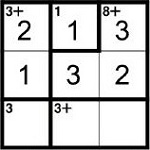
\includegraphics[scale=0.75]{Gambar/Backtracking6}
\caption[Ilustrasi \textit{state} 19 pada sebuah \textit{grid} teka-teki Calcudoku ~\cite{fahda:16:backtracking}]{Ilustrasi \textit{state} 19 pada sebuah \textit{grid} teka-teki Calcudoku ~\cite{fahda:16:backtracking}}
\label{fig:backtracking6}
\end{figure}

\item Langkah berikutnya adalah mulai mengisikan sel-sel yang terletak pada baris ke-3, dari kolom yang paling kiri ke kolom yang paling kanan, dimulai dengan mengisikan \begin{math}x_7\end{math}, yaitu sel pada kolom ke-1 dan baris ke-3 dengan angka 1 (\textit{state} 20), tetapi gagal dalam pemeriksaan kolom, karena angka 1 sudah pernah digunakan dalam kolom tersebut.
\item Langkah berikutnya adalah mencoba kemungkinan angka berikutnya, yaitu angka 2 (\textit{state} 21), tetapi juga gagal dalam pemeriksaan kolom, karena angka 2 sudah pernah digunakan dalam kolom tersebut.
\item Langkah berikutnya adalah mencoba kemungkinan angka berikutnya, yaitu angka 3 (\textit{state} 22), dan ternyata berhasil, sehingga bisa maju ke sel berikutnya, yaitu \begin{math}x_8\end{math}, atau sel pada kolom ke-2 dan baris ke-3.
\item Langkah berikutnya adalah mencoba mengisikan angka 1 pada \begin{math}x_8\end{math} (\textit{state} 23), tetapi gagal dalam pemeriksaan kolom, karena angka 1 sudah pernah digunakan dalam kolom tersebut.
\item Langkah berikutnya adalah mencoba kemungkinan angka berikutnya, yaitu angka 2 (\textit{state} 24), dan ternyata berhasil, sehingga bisa maju ke sel berikutnya, yaitu \begin{math}x_9\end{math}, atau sel pada kolom ke-3 dan baris ke-3.
\item \begin{math}x_9\end{math} adalah sel terakhir, terletak pada sudut kanan bawah \textit{grid}. Langkah berikutnya adalah mencoba mengisikan \begin{math}x_9\end{math} dengan angka 1 (\textit{state} 25), dan ternyata berhasil. Algoritma \textit{backtracking} telah selesai mengisikan seluruh sel dalam \textit{grid} dengan benar. Gambar~\ref{fig:backtracking7} menggambarkan \textit{state} 25 dalam penyelesaian teka-teki Calcudoku ini. Algoritma \textit{backtracking} ini mencapai solusinya pada \textit{state} 25, seperti pada \textit{state space tree} yang digambarkan dalam Gambar~\ref{fig:backtracking8}. \textit{State space tree} ini telah mencapai simpul tujuannya, yaitu simpul 25, dengan jalur 2-1-3-1-3-2-3-2-1.

\begin{figure}
\centering
\captionsetup{justification=centering}
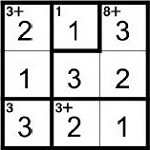
\includegraphics[scale=0.75]{Gambar/Backtracking7}
\caption[\textit{State} 25, simpul tujuan, sebagai hasil yang dicapai ~\cite{fahda:16:backtracking}]{\textit{State} 25, simpul tujuan, sebagai hasil yang dicapai ~\cite{fahda:16:backtracking}}
\label{fig:backtracking7}
\end{figure}

\end{enumerate}

\begin{figure}
\centering
\captionsetup{justification=centering}
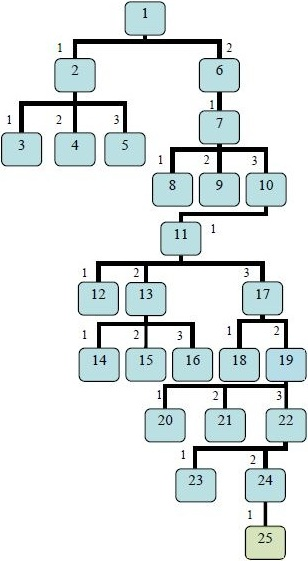
\includegraphics[scale=1]{Gambar/Backtracking8}
\caption[\textit{State space tree} yang dikembangkan dalam proses menyelesaikan teka-teki Calcudoku yang digambarkan pada Gambar~\ref{fig:backtracking4} ~\cite{fahda:16:backtracking}]{\textit{State space tree} yang dikembangkan dalam proses menyelesaikan teka-teki Calcudoku yang digambarkan pada Gambar~\ref{fig:backtracking4} ~\cite{fahda:16:backtracking}}
\label{fig:backtracking8}
\end{figure}

Tinggi pohon yang dikembangkan untuk menyelesaikan sebuah teka-teki dengan ukuran \begin{math}n \times n\end{math} akan memiliki tinggi \begin{math}n^2+1\end{math} saat mencapai simpul tujuannya, dengan jalur dari simpul akar ke simpul tujuan merepresentasikan semua angka yang digunakan untuk mengisi \textit{grid} dari sel pada sudut kiri atas ke sel pada sudut kanan bawah.

Singkatnya, langkah-langkah dasar dari implementasi algoritma \textit{backtracking} dapat dijelaskan sebagai berikut ~\cite{fahda:16:backtracking}:
\begin{enumerate}
\item Carilah sel pertama atau sel yang kosong di dalam \textit{grid}.
\item Isilah sel dengan sebuah angka dimulai dari 1 sampai \begin{math}n\end{math} sampai sebuah angka yang berlaku (\textit{valid}) ditemukan atau sampai angka sudah melebihi \begin{math}n\end{math}.
\item Jika angka untuk sel berlaku, ulangi langkah 1 dan 2.
\item Jika angka untuk sel sudah melebihi \begin{math}n\end{math} dan tidak ada angka dari 1 sampai \begin{math}n\end{math} yang berlaku untuk sel tersebut, mundur ke sel sebelumnya dan cobalah kemungkinan angka berikutnya yang berlaku untul sel tersebut.
\item Jika tidak ada lagi sel yang kosong, solusi sudah ditemukan.
\end{enumerate}

\section{Algoritma \textit{Hybrid Genetic} ~\cite{johanna:12:hybrid}}
\label{sec:hybridgenetic}

Dalam kasus ini, algoritma \textit{hybrid genetic} adalah gabungan dari algoritma \textit{rule based} dan algoritma genetik. Algoritma \textit{rule based} akan dijalankan sampai pada titik dimana algoritma tidak bisa menyelesaikan permainan teka-teki Calcudoku. Jika algoritma sudah tidak bisa menyelesaikan permainan, maka algoritma genetik akan mulai dijalankan.

\subsection{Algoritma \textit{Rule Based}}
\label{sec:rulebased}

Algoritma \textit{rule based} adalah sebuah algoritma berbasis aturan logika untuk menyelesaikan teka-teki Sudoku dan variasinya, termasuk Calcudoku. Beberapa aturan logika yang digunakan dalam algoritma ini adalah \textit{single square rule}, \textit{naked subset rule}, \textit{hidden single rule}, \textit{evil twin rule}, \textit{killer combination}, dan \textit{X-wing} ~\cite{johanna:12:hybrid}.

Aturan \textit{single square} digunakan jika sebuah \textit{cage} hanya berisi satu sel. Hal ini berarti nilai dari sel tersebut sama dengan angka tujuan yang telah ditentukan.

Aturan \textit{naked subset} digunakan jika ada \begin{math}n\end{math} sel dalam kolom atau baris yang sama yang mempunyai \begin{math}n\end{math} kemungkinan nilai yang sama persis untuk mengisikannya, dengan \begin{math}n \geq 2 \end{math}. Hal ini berarti sel-sel lainnya dalam baris dan kolom tersebut tidak mungkin diisi dengan nilai yang sama dengan nilai milik \begin{math}n\end{math} sel tersebut. Gambar~\ref{fig:hybrid2} menunjukkan bagaimana cara kerja aturan ini. Sel-sel pada kolom ke-4 dan ke-6 mempunyai tepat dua kemungkinan nilai (1 atau 7). Ini disebut sebagai \textit{naked pair}. Karena angka 1 dan 7 harus diisi pada sel-sel pada kolom ke-4 dan ke-6, maka angka 1 dan 7 bisa dieliminasi dari sel-sel pada kolom ke-7 dan ke-8.

\begin{figure}
\centering
\captionsetup{justification=centering}
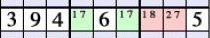
\includegraphics[scale=1]{Gambar/HybridGenetic2}
\caption[Contoh bagaimana cara mendeteksi aturan \textit{naked pair} ~\cite{johanna:12:hybrid}]{Contoh bagaimana cara mendeteksi aturan \textit{naked pair} ~\cite{johanna:12:hybrid}}
\label{fig:hybrid2}
\end{figure}

Aturan \textit{evil twin} digunakan jika sebuah \textit{cage} berisikan dua sel, dan salah satu dari kedua sel sudah terisi, maka sel yang satunya lagi diisi dengan angka yang jika kedua angka dihitung dengan operasi matematika yang ditentukan maka akan menghasilkan angka tujuan yang ditentukan. Aturan ini adalah aturan yang paling mudah. Kenyataannya, aturan ini bisa digeneralisasikan untuk \textit{cage} yang berukuran lebih dari 2 sel. Sel yang belum terisi yang terakhir dalam sebuah area diisi oleh sebuah nilai yang diperlukan untuk mencapai nilai tujuan menggunakan operasi matematika yang telah ditentukan. Contohnya, pada Gambar~\ref{fig:hybrid3}, begitu sel di sudut kiri bawah diisi oleh angka 4, maka sel diatasnya harus diisi oleh angka 9.

\begin{figure}
\centering
\captionsetup{justification=centering}
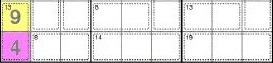
\includegraphics[scale=1]{Gambar/HybridGenetic3}
\caption[Contoh aturan \textit{evil twin} ~\cite{johanna:12:hybrid}]{Contoh aturan \textit{evil twin} ~\cite{johanna:12:hybrid}}
\label{fig:hybrid3}
\end{figure}

Aturan \textit{hidden single} digunakan jika sebuah angka hanya bisa diisikan dalam satu sel dalam sebuah baris atau kolom. Aturan ini secara konsep cukup mudah, tetapi kadang-kadang sulit untuk diamati. Pada Gambar~\ref{fig:hybrid4}, nilai-nilai yang mungkin untuk sel yang paling kiri adalah 3, 5, dan 7, tetapi dalam baris ini, angka 7 harus muncul dalam salah satu selnya, dan hanya sel yang paling kiri tersebut yang memiliki kemungkinan nilai 7. Ini disebut sebagai \textit{hidden single}. Sel tersebut harus diisi dengan angka 7.

\begin{figure}
\centering
\captionsetup{justification=centering}
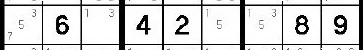
\includegraphics[scale=1]{Gambar/HybridGenetic4}
\caption[Contoh aturan \textit{hidden single} ~\cite{johanna:12:hybrid}]{Contoh aturan \textit{hidden single} ~\cite{johanna:12:hybrid}}
\label{fig:hybrid4}
\end{figure}

Aturan \textit{killer combination} adalah aturan yang paling krusial. Aturan ini digunakan jika sebuah \textit{cage} berisikan sel-sel yang berada dalam baris atau kolom yang sama dan operasi yang ditentukan adalah penjumlahan. Kemungkinan angka yang unik untuk aturan \textit{killer combination} berhubungan dengan ukuran \textit{cage}. Contoh, jika sebuah \textit{cage} memiliki dua sel dan angka tujuannya adalah 3, maka kemungkinan angka yang bisa diisikan ke dalam kedua sel tersebut adalah 1 atau 2. Hal ini berarti semua angka lainnya tidak mungkin diisikan ke dalam kedua sel tersebut. Contoh lain, jika sebuah \textit{cage} memiliki tiga sel dan angka tujuannya adalah 24, maka kemungkinan angka yang bisa diisikan ke dalam ketiga sel tersebut adalah 7, 8, atau 9. Gambar~\ref{fig:hybrid5} menampilkan contoh penerapan aturan \textit{killer combination} untuk \textit{cage} dengan ukuran 2 sel. Tabel ini juga bisa diperluas untuk ukuran \textit{cage} lainnya.

\begin{figure}
\centering
\captionsetup{justification=centering}
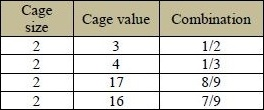
\includegraphics[scale=1]{Gambar/HybridGenetic5}
\caption[Contoh aturan \textit{killer combination} untuk \textit{cage} dengan ukuran 2 sel dengan operasi matematika penjumlahan~\cite{johanna:12:hybrid}]{Contoh aturan \textit{killer combination} untuk \textit{cage} dengan ukuran 2 sel dengan operasi matematika penjumlahan~\cite{johanna:12:hybrid}}
\label{fig:hybrid5}
\end{figure}

Aturan \textit{X-wing} digunakan jika hanya ada dua kemungkinan angka yang bisa diisikan ke dalam dua sel yang berada di dalam dua baris yang berbeda, dan dua kemungkinan angka tersebut juga berada di dalam kolom yang sama maka sel-sel lainnya dalam kolom tersebut tidak mungkin diisi oleh dua kemungkinan angka tersebut, atau jika hanya ada dua kemungkinan angka yang bisa diisikan ke dalam dua sel yang berada di dalam dua kolom yang berbeda, dan dua kemungkinan angka tersebut juga berada di dalam baris yang sama maka sel-sel lainnya dalam baris tersebut tidak mungkin diisi oleh dua kemungkinan angka tersebut. Gambar~\ref{fig:hybrid6} menampilkan contoh penggunaan aturan \textit{X-wing}. Misalnya, jika sel A diisi oleh angka 7, maka angka 7 akan dieliminasi dari sel B dan sel C. Karena sel A dengan sel C dan sel D 'terkunci', maka sel D harus diisi oleh angka 7. Jadi, angka 7 harus di isi pada sel A dan sel D atau pada sel B dan sel C. Angka 7 bisa dieliminasi dari sel-sel yang berwarna hijau.

\begin{figure}
\centering
\captionsetup{justification=centering}
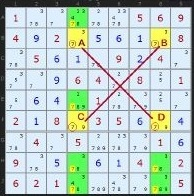
\includegraphics[scale=1]{Gambar/HybridGenetic6}
\caption[Contoh aturan \textit{X-wing} ~\cite{johanna:12:hybrid}]{Contoh aturan \textit{X-wing} ~\cite{johanna:12:hybrid}}
\label{fig:hybrid6}
\end{figure}

\subsection{Algoritma Genetik}
\label{sec:genetik}

Pencarian heuristik adalah sebuah teknik pencarian kecerdasan buatan (\textit{artifical intelligence}) yang menggunakan heuristik dalam langkah-langkahnya. Heuristik adalah semacam aturan tidak tertulis yang mungkin menghasilkan solusi. Heuristik kadang-kadang efektif, tetapi tidak dijamin akan berhasil. dalam setiap kasus. Heuristik memerankan peran penting dalam strategi pencarian karena sifat eksponensial dari kebanyakan masalah. Heuristik membantu mengurangi jumlah alternatif solusi dari angka yang bersifat eksponensial menjadi angka yang bersifat polinomial. Contoh teknik pencarian heuristik adalah \textit{Generate and Test}, \textit{Hill Climbing}, dan \textit{Best First Search}.

Algoritma genetik adalah salah satu teknik heuristik \textit{Generate and Test} yang terinspirasi oleh sistem seleksi alam. Algoritma ini adalah perpaduan dari bidang biologi dan ilmu komputer. Algoritma ini memanipulasi informasi, biasanya disebut sebagai kromosom. Kromosom ini meng-\textit{encode} kemungkinan jawaban untuk sebuah masalah yang diberikan. Kromosom dievaluasi dan diberi \textit{fitness value} berdasarkan seberapa baik kromosom dalam menyelesaikan masalah yang diberikan berdasarkan kriteria yang ditentukan oleh pembuat program. Nilai kelayakan ini digunakan sebagai probabilitas kebertahanan hidup kromosom dalam satu siklus reproduksi. Kromosom baru (kromosom anak, \textit{child chromosome}) diproduksi dengan menggabungkan dua (atau lebih) kromosom orang tua (\textit{parent chromosome}). Proses ini dirancang untuk menghasilkan kromosom-kromosom keturunan yang lebih layak, kromosom-kromosom ini meng-\textit{encode} jawaban yang lebih baik, sampai solusi yang baik dan yang bisa diterima ditemukan.

Cara kerja algoritma genetik adalah sebagai berikut ~\cite{johanna:12:hybrid}:
\begin{enumerate}
\item Menentukan populasi kromosom kemungkinan jawaban awal.
\item Membangkitkan populasi kemungkinan jawaban awal secara acak.
\item Mengevaluasi fungsi objektif.
\item Melakukan operasi terhadap kromosom menggunakan operator genetik (reproduksi, kawin silang, dan mutasi).
\item Ulangi langkah 3 dan 4 sampai mencapai kriteria untuk menghentikan algoritma.
\end{enumerate}
Langkah-langkah utama dalam penggunaan algoritma genetik adalah membangkitkan populasi kemungkinan jawaban, mencari fungsi objektif dan fungsi kelayakan, dan penggunaan operator genetik.

\clearpage

\subsection{Algoritma \textit{Hybrid Genetic}}
\label{sec:subhybrid}

Pencarian \textit{rule based} dimulai dengan mengasumsikan semua nilai sel yang tidak diketahui dengan semua kemungkinan nilai untuk mengisi sel tersebut tanpa melanggar batasan, dengan \begin{math}P(C_{b,k}) = {1, 2, ..., n}\end{math}. Setelah nilai dari satu sel sudah ditentukan, kemungkinan nilai untuk beberapa sel tertentu diperbaharui. Misalnya, penggunaan aturan \textit{naked single} yang dinyatakan dalam persamaan 1 di bawah ini, akan mengakibatkan semua kemungkinan nilai untuk semua sel lain dalam baris yang sama dan dalam kolom yang sama harus diperbaharui, seperti dinyatakan dalam persamaan 2 dan 3 di bawah ini. Aturan \textit{naked pair}, salah satu dari aturan jenis \textit{naked subset}, dinyatakan dalam persamaan 4 untuk baris dan persamaan 5 untuk kolom. ~\cite{johanna:12:hybrid}

\begin{enumerate}
\item \begin{math}|P(C_{b,k})| = 1 \land x \in P(C_{b,k}) \rightarrow V(C_{b,k}) = x\end{math}, artinya jika sebuah \textit{cage} berukuran 1 sel, dan \begin{math}x\end{math} adalah nilai tujuan dari \textit{cage} tersebut, maka nilai dari sel tersebut adalah \begin{math}x\end{math}.
\item \begin{math}(V(C_{b,k}) = x) \land (\forall a \in \{1, 2, ..., n\}) \rightarrow P(C_{a,k}) = P(C_{a,k}) - \{x\}\end{math}, artinya jika nilai suatu sel pada baris \begin{math}b\end{math} dan kolom \begin{math}k\end{math} adalah \begin{math}x\end{math}, maka \begin{math}x\end{math} dihapus dari kemungkinan angka-angka yang bisa digunakan untuk mengisi sel-sel lain pada baris \begin{math}b\end{math}.
\item \begin{math}(V(C_{b,k}) = x) \land (\forall q \in \{1, 2, ..., n\}) \rightarrow P(C_{b,q}) = P(C_{b,q}) - \{x\}\end{math} artinya jika nilai suatu sel pada baris \begin{math}b\end{math} dan kolom \begin{math}k\end{math} adalah \begin{math}x\end{math}, maka \begin{math}x\end{math} dihapus dari kemungkinan angka-angka yang bisa digunakan untuk mengisi sel-sel lain pada kolom \begin{math}k\end{math}.
\item \begin{math}|P(C_{b,k1})| = |P(C_{b,k2})| = 2 \land P(C_{b,k1}) = P(C_{b,k2}) \rightarrow P(C_{b,q}) = P(C_{b,q}) - P(C_{b,k1})\end{math}, artinya jika ada dua sel dalam satu baris yang hanya bisa diisi oleh dua kemungkinan angka, maka kedua angka tersebut dihapus dari kemungkinan angka-angka yang bisa digunakan untuk mengisi sel-sel lain pada baris tersebut.
\item \begin{math}|P(C_{b1,k})| = |P(C_{b2,k})| = 2 \land P(C_{b1,k}) = P(C_{b2,k}) \rightarrow P(C_{p,k}) = P(C_{p,k}) - P(C_{b1,k})\end{math}, artinya jika ada dua sel dalam satu kolom yang hanya bisa diisi oleh dua kemungkinan angka, maka kedua angka tersebut dihapus dari kemungkinan angka-angka yang bisa digunakan untuk mengisi sel-sel lain pada kolom tersebut.
\end{enumerate}

Algoritma genetik digunakan saat teka-teki masih tidak bisa diselesaikan setelah mengerjakan semua aturan logika secara berulang-ulang. Algoritma ini dimulai dengan meng-\textit{encode} kromosom. Satu kromosom terdiri dari \begin{math}k\end{math} segmen, dengan \begin{math}m \leq n\end{math}. Satu segmen berisikan sekumpulan gen yang belum diselesaikan yang berada di dalam segmen tersebut. Sebuah segmen merepresentasikan sebuah baris atau kolom. Dalam sebuah kromosom, segmen diurutkan dari baris yang paling atas ke baris yang paling bawah atau dari kolom yang paling kiri ke kolom yang paling kanan. Contoh, salah satu kromosom dari permainan teka-teki Calcudoku pada Gambar~\ref{fig:hybrid8} adalah:

\begin{math}34 \ 35 \ | \ 28 \ 29 \ 24 \ 25 \ | \ 0 \ 4 \ 5 \ 1 \ 2 \ 3 \ | \ 11 \ 6 \ 9 \ 7 \ 8 \ 10 \ | \ 12 \ 14 \ 15 \ 17 \ 16 \ 13 \ | \ 20 \ 18 \ 19 \ 23 \ 21 \ 22\end{math}

Setiap segmen dalam contoh kromosom ini merepresentasikan sebuah baris yang belum terselesaikan.

\begin{figure}
\centering
\captionsetup{justification=centering}
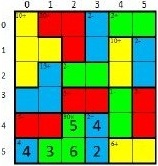
\includegraphics[scale=1]{Gambar/HybridGenetic8}
\caption[Contoh permainan teka-teki Calcudoku dengan ukuran \textit{grid} 6 x 6~\cite{johanna:12:hybrid}]{Contoh permainan teka-teki Calcudoku dengan ukuran \textit{grid} 6 x 6 ~\cite{johanna:12:hybrid}}
\label{fig:hybrid8}
\end{figure}

Fungsi objektif, yang direpresentasikan dengan \begin{math}x_j\end{math}, akan dihitung setelah pembangkitan nilai dari gen pada kromosom sudah dilakukan. Nilai untuk gen ke-\begin{math}j\end{math} pada sebuah kromosom direpresentasikan dengan \begin{math}w_j\end{math}. \begin{math}x_j\end{math} akan bernilai 0 jika belum diselesaikan (\begin{math}w_j = 0\end{math}), dan bernilai 1 jika sudah diselesaikan (\begin{math}w_j \neq 0\end{math}). Untuk kromosom dengan jumlah gen \begin{math}k\end{math}, fungsi kelayakan, yaitu hasil penjumlahan dari hasil fungsi objektif untuk setiap gen dibagi dengan jumlah gen, dinyatakan dalam persamaan di bawah ini ~\cite{johanna:12:hybrid}:
\begin{displaymath}
x_j = 
\begin{cases}
0, w_j = 0 \\
1, w_j \neq 0
\end{cases}
\end{displaymath}
\begin{displaymath}
fitness = \frac{\sum_{j=0}^k x_j}{k}
\end{displaymath}
Jadi, solusi dari teka-teki ini adalah mencari kromosom yang nilai kelayakannya 1.

Dalam proses reproduksi kawin silang, dua kromosom, yaitu kromosom orang tua, disilangkan untuk membuat dua kromosom yang baru, yaitu kromosom anak, dengan metodologi kawin silang \textit{\begin{math}N\end{math}-segments}. Gambar~\ref{fig:hybrid9} menggambarkan contoh proses kawin silang antara dua kromosom.

\begin{figure}
\centering
\captionsetup{justification=centering}
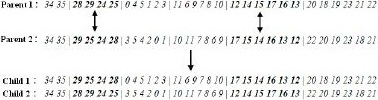
\includegraphics[scale=1]{Gambar/HybridGenetic9}
\caption[Contoh proses kawin silang antara dua kromosom ~\cite{johanna:12:hybrid}]{Contoh proses kawin silang antara dua kromosom ~\cite{johanna:12:hybrid}}
\label{fig:hybrid9}
\end{figure}

Pertukaran mutasi digunakan untuk mendapatkan kemungkinan kromosom yang lain. Mutasi dilakukan di antara gen yang berada dalam segmen yang sama. Gambar~\ref{fig:hybrid10} adalah contoh proses mutasi antara dua gen dalam segmen yang sama.

\begin{figure}
\centering
\captionsetup{justification=centering}
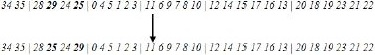
\includegraphics[scale=1]{Gambar/HybridGenetic10}
\caption[Contoh proses mutasi ~\cite{johanna:12:hybrid}]{Contoh proses mutasi ~\cite{johanna:12:hybrid}}
\label{fig:hybrid10}
\end{figure}

Cara kerja algoritma \textit{hybrid genetic} adalah sebagai berikut ~\cite{johanna:12:hybrid}:
\begin{enumerate}
\item Masukkan teka-teki yang akan diselesaikan sebagai input. Teka-teki Calcudoku diinputkan oleh pemain dalam bentuk \textit{file}.
\item Representasikan input yang dimasukkan ke dalam format teka-teki Calcudoku. File teka-teki Calcudoku yang telah diinputkan oleh pemain ditampilkan ke layar sebagai teka-teki Calcudoku.
\item Algoritma \textit{hybrid genetic} akan mencoba menyelesaikan teka-teki tersebut dengan menggunakan algoritma \textit{rule based} terlebih dahulu.
\item Jika berhasil menyelesaikan teka-teki tersebut dengan menggunakan algoritma \textit{rule based}, maka algoritma selesai.
\item Jika gagal dengan menggunakan algoritma \textit{rule based}, maka algoritma \textit{hybrid genetic} akan mencoba menyelesaikan teka-teki tersebut dengan menggunakan algoritma genetik.
\item Jika berhasil menyelesaikan teka-teki tersebut dengan menggunakan algoritma genetik, maka algoritma selesai.
\item Jika gagal dalam menyelesaikan teka-teki tersebut setelah menggunakan algoritma genetik, artinya algoritma \textit{hybrid genetic} gagal dalam menyelesaikan teka-teki terseebut.
\end{enumerate}
Alur (\textit{flow chart}) penyelesaian permainan teka-teki Calcudoku dengan menggunakan algoritma \textit{hybrid genetic} dapat dilihat di Gambar~\ref{fig:hybrid7}.

\begin{figure}
\centering
\captionsetup{justification=centering}
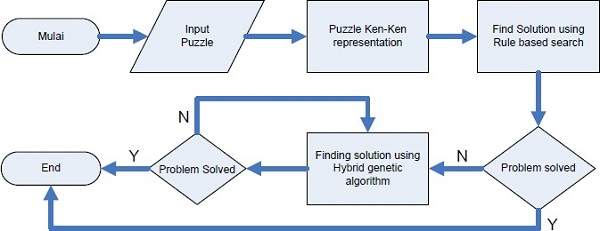
\includegraphics[scale=1]{Gambar/HybridGenetic7}
\caption[Alur penyelesaian permainan teka-teki Calcudoku dengan menggunakan algoritma \textit{hybrid genetic} ~\cite{johanna:12:hybrid}]{Alur penyelesaian permainan teka-teki Calcudoku dengan menggunakan algoritma \textit{hybrid genetic} ~\cite{johanna:12:hybrid}}
\label{fig:hybrid7}
\end{figure}}{}
\ifdefstring{\vbabc}{1}{\chapter{Analisis}
\label{chap:analisis}

Bab ini membahas tentang analisis cara kerja algoritma \textit{backtracking} dan algoritma \textit{hybrid genetic} untuk menyelesaikan permainan teka-teki Calcudoku, dan analisis kebutuhan perangkat lunak Calcudoku.

\section{Analisis Algoritma \textit{Backtracking}}
\label{sec:analisisbt}

Langkah-langkah penyelesaian permainan teka-teki Calcudoku dengan menggunakan algoritma \textit{backtracking} secara umum adalah sebagai berikut:

\begin{enumerate}
\item Isilah \textit{grid} mulai dari sel pada sudut kiri atas.
\item Setelah mengisi sebuah sel, isilah sel di sebelah kanannya.
\item Jika sudah mengisi sel yang paling kanan, isilah sel yang paling kiri pada baris berikutnya.
\item Jika semua kemungkinan gagal, mundur ke langkah sebelumnya, dan cobalah kemungkinan berikutnya.
\item Algoritma \textit{backtracking} selesai jika semua sel sudah terisi dengan benar.
\end{enumerate}

Untuk mengilustrasikan cara kerja algoritma \textit{backtracking}, akan digunakan permainan teka-teki Calcudoku yang digambarkan pada Gambar~\ref{fig:analisisbt1} sebagai contoh. \textit{State space tree} seperti yang dijelaskan pada Bab~\ref{sec:backtracking} akan dibangkitkan.

\begin{figure}
\centering
\captionsetup{justification=centering}
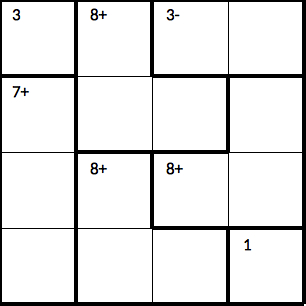
\includegraphics[scale=0.333]{Gambar/backtracking/State1}
\caption[Contoh permainan teka-teki Calcudoku dengan ukuran \textit{grid} 4 x 4 yang belum diselesaikan, seperti yang digambarkan pada Gambar~\ref{fig:backtracking1}. ~\cite{fahda:16:backtracking}]{Contoh permainan teka-teki dengan ukuran \textit{grid} 4 x 4 yang belum diselesaikan, seperti yang digambarkan pada Gambar~\ref{fig:backtracking1}. ~\cite{fahda:16:backtracking}}
\label{fig:analisisbt1}
\end{figure}

\begin{enumerate}
\item Algoritma \textit{backtracking} dimulai dengan teka-teki yang belum diselesaikan, seperti yang digambarkan pada Gambar~\ref{fig:analisisbt1} (\textit{state} 1).
\item Algoritma mengisikan sel pada baris ke-1 dan kolom ke-1 dengan angka 1 (\textit{state} 2), tetapi angka 1 tidak sesuai dengan angka tujuan dari \textit{cage} tersebut.
\item Algoritma lalu mencoba kemungkinan angka berikutnya, yaitu angka 2 (\textit{state} 3), tetapi angka 2 juga tidak sesuai dengan angka tujuan dari \textit{cage} tersebut.
\item Algoritma lalu mencoba kemungkinan angka berikutnya, yaitu angka 3 (\textit{state} 4), seperti dapat dilihat pada Gambar~\ref{fig:analisisbt2}, dan ternyata angka 3 sesuai dengan angka tujuan dari \textit{cage} tersebut, sehingga algoritma dapat maju ke sel berikutnya.

\begin{figure}
\centering
\captionsetup{justification=centering}
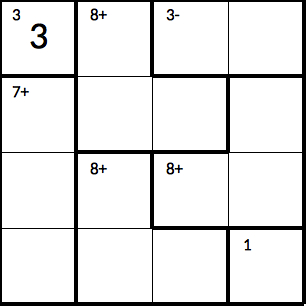
\includegraphics[scale=0.333]{Gambar/backtracking/State4}
\caption[\textit{State} 4]{\textit{State} 4}
\label{fig:analisisbt2}
\end{figure}

\item Algoritma lalu mengisikan sel pada baris ke-1 dan kolom ke-2 dengan angka 1 (\textit{state} 5). Algoritma lalu maju ke sel berikutnya.
\item Algoritma lalu mengisikan sel pada baris ke-1 dan kolom ke-3 dengan angka 1 (\textit{state} 6), tetapi angka 1 sudah pernah digunakan dalam baris tersebut.
\item Algoritma lalu mencoba kemungkinan angka berikutnya, yaitu angka 2 (\textit{state} 7). Algoritma lalu maju ke sel berikutnya.
\item Algoritma lalu mengisikan sel pada baris ke-1 dan kolom ke-4 dengan angka 1 (\textit{state} 8), tetapi angka 1 sudah pernah digunakan dalam baris tersebut.
\item Algoritma lalu mencoba kemungkinan angka berikutnya, yaitu angka 2 (\textit{state} 9), tetapi angka 2 sudah pernah digunakan dalam baris tersebut.
\item Algoritma lalu mencoba kemungkinan angka berikutnya, yaitu angka 3 (\textit{state} 10), tetapi angka 3 sudah pernah digunakan dalam baris tersebut.
\item Algoritma lalu mencoba kemungkinan angka berikutnya, yaitu angka 4 (\textit{state} 11), seperti dapat dilihat pada Gambar~\ref{fig:analisisbt3}, tetapi hasilnya tidak sesuai dengan angka tujuan dari \textit{cage} tersebut.

\begin{figure}
\centering
\captionsetup{justification=centering}
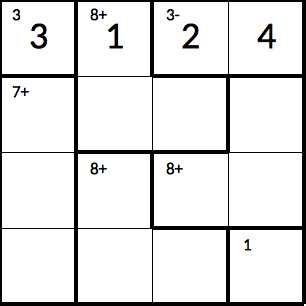
\includegraphics[scale=0.333]{Gambar/backtracking/State11}
\caption[\textit{State} 11]{\textit{State} 11}
\label{fig:analisisbt3}
\end{figure}

\item Karena semua kemungkinan angka untuk baris ke-1 dan kolom ke-4 telah dicoba dan gagal, maka algoritma harus mundur kembali ke (\textit{state} 7). Algoritma mencoba kemungkinan angka berikutnya, yaitu angka 3 (\textit{state} 12), seperti dapat dilihat pada Gambar~\ref{fig:analisisbt4}, tetapi angka 3 sudah pernah digunakan dalam baris tersebut.

\begin{figure}
\centering
\captionsetup{justification=centering}
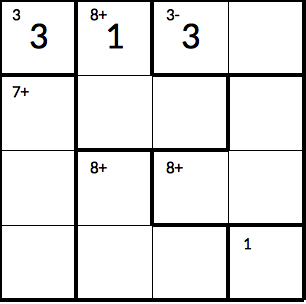
\includegraphics[scale=0.333]{Gambar/backtracking/State12}
\caption[\textit{State} 12]{\textit{State} 12}
\label{fig:analisisbt4}
\end{figure}

\item Algoritma lalu mencoba kemungkinan angka berikutnya, yaitu angka 4 (\textit{state} 13). Algoritma lalu maju ke sel berikutnya.
\item Algoritma lalu mengisikan sel pada baris ke-1 dan kolom ke-4 dengan angka 1 (\textit{state} 14), tetapi angka 1 sudah pernah digunakan dalam baris tersebut.
\item Algoritma lalu mencoba kemungkinan angka berikutnya, yaitu angka 2 (\textit{state} 15), tetapi hasilnya tidak sesuai dengan angka tujuan dari \textit{cage} tersebut.
\item Algoritma lalu mencoba kemungkinan angka berikutnya, yaitu angka 3 (\textit{state} 16), tetapi angka 3 sudah pernah digunakan dalam baris tersebut.
\item Algoritma lalu mencoba kemungkinan angka berikutnya, yaitu angka 4 (\textit{state} 17), seperti dapat dilihat pada Gambar~\ref{fig:analisisbt5}, tetapi angka 4 sudah pernah digunakan dalam baris tersebut.

\begin{figure}
\centering
\captionsetup{justification=centering}
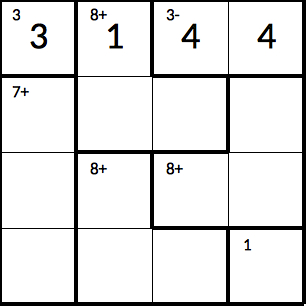
\includegraphics[scale=0.333]{Gambar/backtracking/State17}
\caption[\textit{State} 17]{\textit{State} 17}
\label{fig:analisisbt5}
\end{figure}

\item Karena semua kemungkinan angka untuk baris ke-1 dan kolom ke-3 dan ke-4 telah dicoba dan gagal, maka algoritma harus mundur kembali ke (\textit{state} 5). Algoritma mencoba kemungkinan angka berikutnya, yaitu angka 2 (\textit{state} 18), seperti dapat dilihat pada Gambar~\ref{fig:analisisbt6}. Algoritma lalu maju ke sel berikutnya.

\begin{figure}
\centering
\captionsetup{justification=centering}
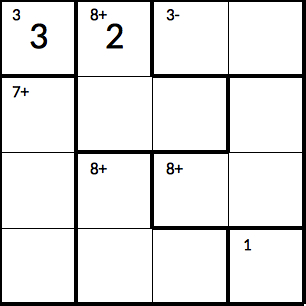
\includegraphics[scale=0.333]{Gambar/backtracking/State18}
\caption[\textit{State} 18]{\textit{State} 18}
\label{fig:analisisbt6}
\end{figure}

\item Algoritma lalu mengisikan sel pada baris ke-1 dan kolom ke-3 dengan angka 1 (\textit{state} 19), seperti dapat dilihat pada Gambar~\ref{fig:analisisbt7}. Algoritma lalu maju ke sel berikutnya.

\begin{figure}
\centering
\captionsetup{justification=centering}
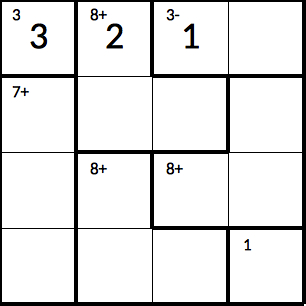
\includegraphics[scale=0.333]{Gambar/backtracking/State19}
\caption[\textit{State} 19]{\textit{State} 19}
\label{fig:analisisbt7}
\end{figure}

\item Algoritma lalu mengisikan sel pada baris ke-1 dan kolom ke-4 dengan angka 1 (\textit{state} 20), tetapi angka 1 sudah pernah digunakan dalam baris tersebut.
\item Algoritma lalu mencoba kemungkinan angka berikutnya, yaitu angka 2 (\textit{state} 21), tetapi angka 2 sudah pernah digunakan dalam baris tersebut.
\item Algoritma lalu mencoba kemungkinan angka berikutnya, yaitu angka 3 (\textit{state} 22), tetapi angka 3 sudah pernah digunakan dalam baris tersebut.
\item Algoritma lalu mencoba kemungkinan angka berikutnya, yaitu angka 4 (\textit{state} 23), dan ternyata hasilnya sesuai dengan angka tujuan dari \textit{cage} tersebut, seperti dapat dilihat pada Gambar~\ref{fig:analisisbt8}. Algoritma telah selesai mengisikan baris ke-1, sehingga bisa maju ke baris berikutnya.

\begin{figure}
\centering
\captionsetup{justification=centering}
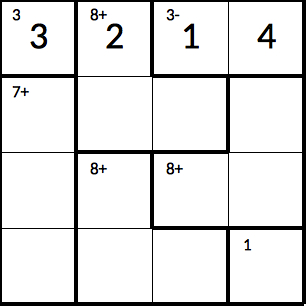
\includegraphics[scale=0.333]{Gambar/backtracking/State23}
\caption[\textit{State} 23]{\textit{State} 23}
\label{fig:analisisbt8}
\end{figure}

\item Langkah-langkah di atas diulang untuk mengisi sel-sel pada baris-baris selanjutnya. Algoritma \textit{backtracking} berhasil mengisi semua sel dalam permainan teka-teki Calcudoku ini dengan benar pada \textit{state} 93, seperti dapat dilihat pada Gambar~\ref{fig:analisisbt32}.

\begin{figure}
\centering
\captionsetup{justification=centering}
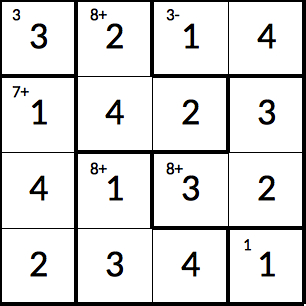
\includegraphics[scale=0.333]{Gambar/backtracking/State93}
\caption[\textit{State} 93]{\textit{State} 93}
\label{fig:analisisbt32}
\end{figure}

\end{enumerate}

Algoritma ini mencapai solusinya pada state 93, seperti pada \textit{state space tree} yang digambarkan dalam Gambar~\ref{fig:analisisbt33}. \textit{State space tree} ini telah mencapai simpul tujuannya, yaitu simpul 93, dengan jalur 3-2-1-4-1-4-2-3-4-1-3-2-2-3-4-1. Penjelasan tentang analisis algoritma \textit{backtracking} secara lengkap dapat dilihat di Lampiran~\ref{chap:analisisbacktracking}.

\begin{landscape}
\begin{figure}
\centering
\captionsetup{justification=centering}
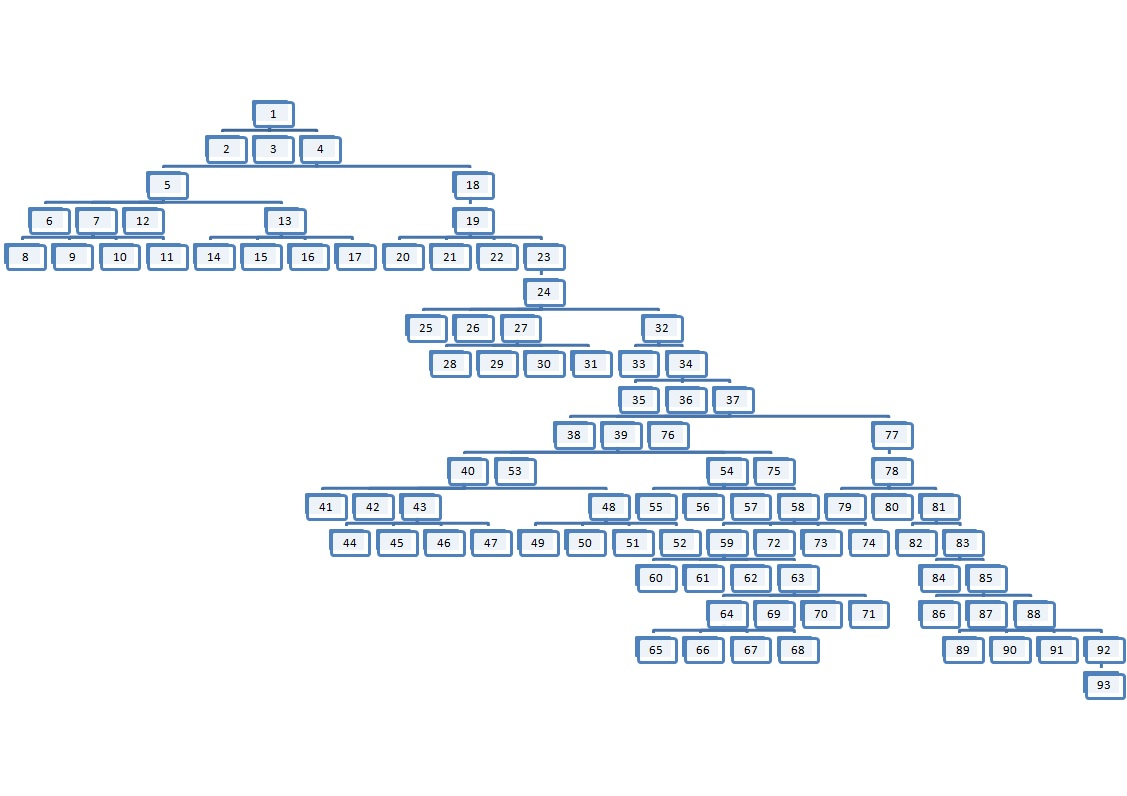
\includegraphics[scale=0.75]{Gambar/backtracking/StateSpaceTree}
\caption[\textit{State space tree} yang dikembangkan dalam proses menyelesaikan teka-teki Calcudoku yang digambarkan pada Gambar~\ref{fig:analisisbt1}]{\textit{State space tree} yang dikembangkan dalam proses menyelesaikan teka-teki Calcudoku yang digambarkan pada Gambar~\ref{fig:analisisbt1}}
\label{fig:analisisbt33}
\end{figure}
\end{landscape}

\section{Analisis Algoritma \textit{Hybrid Genetic}}
\label{sec:analisishg}

Langkah-langkah penyelesaian permainan teka-teki Calcudoku dengan menggunakan algoritma \textit{backtracking} secara umum adalah sebagai berikut:

\begin{enumerate}
\item \textit{Solver} akan mencoba menyelesaikan permainan dengan algoritma \textit{rule based}.
	\begin{enumerate}
	\item Algoritma \textit{rule based} dimulai dengan mengaplikasikan aturan logika \textit{single square} dan aturan logika \textit{killer combination}. Kedua aturan logika ini hanya diaplikasikan sekali, yaitu di awal algoritma.
	\item Algoritma lalu mengaplikasikan aturan logika naked subset dan aturan logika \textit{hidden single}. Kedua aturan logika ini diulang sampai algoritma tidak bisa lagi mengisi sel-sel dalam \textit{grid} atau sampai semua sel dalam \textit{grid} sudah terisi dengan benar.
	\item Algoritma \textit{hybrid genetic} selesai jika semua sel dalam \textit{grid} sudah terisi dengan benar.
        \item Algoritma genetik akan dimulai jika ada sel-sel di dalam \textit{grid} yang masih kosong.
	\end{enumerate}
\item Jika algoritma \textit{rule based} tidak berhasil mengisi semua sel dalam \textit{grid} dengan benar, maka \textit{solver} akan mencoba menyelesaikan permainan dengan algoritma genetik.
	\begin{enumerate}
	\item Algoritma genetik dimulai dengan membangkitkan generasi awal secara acak.
	\item Setiap kromosom dalam sebuah generasi dihitung nilai kelayakannya. Nilai kelayakan untuk sebuah kromosom adalah jumlah sel yang sudah diisi dengan benar dibagi dengan jumlah semua sel yang ada di dalam \textit{grid}.
	\item Algoritma selesai jika solusi ditemukan. Solusi adalah kromosom dengan nilai kelayakan 1.
	\item Jika solusi tidak ditemukan, maka algoritma genetik akan membangkitkan generasi berikutnya, sampai solusi ditemukan. Generasi berikutnya dibangkitkan dari generasi sebelumnya menggunakan operator-operator algoritma genetik, seperti \textit{elitism}, kawin silang, dan mutasi.
	\end{enumerate}
\end{enumerate}

Untuk mengilustrasikan cara kerja algoritma \textit{hybrid genetic}, akan digunakan permainan teka-teki Calcudoku yang digambarkan pada Gambar~\ref{fig:analisishg1} sebagai contoh. Algoritma \textit{hybrid genetic} dimulai dengan mencoba menyelesaikan permainan teka-teki Calcudoku dengan algoritma \textit{rule based}.

\begin{figure}
\centering
\captionsetup{justification=centering}
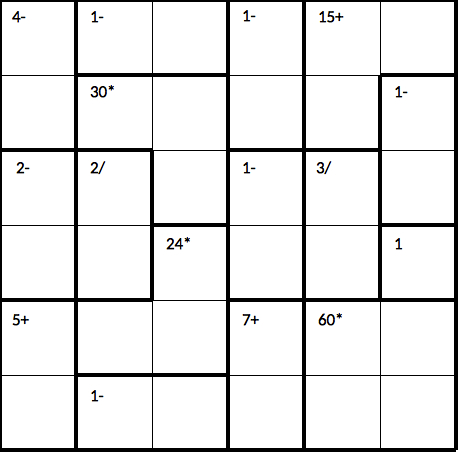
\includegraphics[scale=0.333]{Gambar/hybridgenetic/Puzzle}
\caption[Contoh permainan teka-teki Calcudoku dengan ukuran \textit{grid} 6 x 6 yang belum diselesaikan, seperti yang digambarkan pada Gambar~\ref{fig:hybrid1}. \cite{johanna:12:hybrid}]{Contoh permainan teka-teki Calcudoku dengan ukuran \textit{grid} 6 x 6 yang belum diselesaikan, seperti yang digambarkan pada Gambar~\ref{fig:hybrid1}. \cite{johanna:12:hybrid}}
\label{fig:analisishg1}
\end{figure}

\subsection{Algoritma \textit{Rule Based}}
\label{sec:analisisrb}

Sel pada baris ke-4 dan kolom ke-6 adalah bagian dari sebuah \textit{cage} yang berukuran hanya 1 sel, dan oleh karena itu, angka tujuan dari sel tersebut adalah angka tujuan dari \textit{cage} tersebut (aturan \textit{single square}). Angka tujuan dari \textit{cage} tersebut adalah 1, dan oleh karena itu sel tersebut dapat langsung diisi dengan angka 1, seperti dapat dilihat pada Gambar~\ref{fig:analisishg2}.

Sayangnya, algoritma \textit{rule based} gagal dalam mengisi sel-sel lainnya berdasarkan aturan-aturan yang telah didefinisikan setelah beberapa kali percobaan, sehingga algoritma \textit{hybrid genetic} akan mencoba menyelesaikan teka-teki Calcudoku dengan algoritma genetik.

\begin{figure}
\centering
\captionsetup{justification=centering}
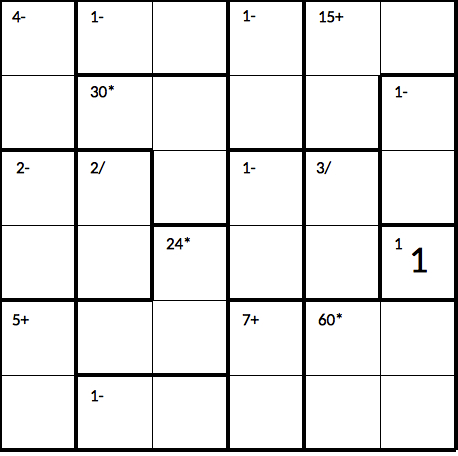
\includegraphics[scale=0.333]{Gambar/hybridgenetic/PuzzleAfterRuleBased}
\caption[Permainan teka-teki Calcudoku setelah diselesaikan dengan algoritma \textit{rule based}]{Permainan teka-teki Calcudoku setelah diselesaikan dengan algoritma \textit{rule based}}
\label{fig:analisishg2}
\end{figure}

\subsection{Algoritma Genetik}
\label{sec:analisisgenetik}

Dalam contoh ini, parameter-parameter untuk algoritma genetik yang akan digunakan untuk teka-teki Calcudoku ini ditunjukkan pada Tabel~\ref{tab:analisishg1}. Dalam kasus ini, parameter ditentukan oleh pembuat program (penulis). Setiap generasi terdiri dari 12 kromosom. \begin{math}40\% \times 12 \approx 5\end{math} kromosom diambil dari generasi sebelumnya (\textit{elitism}). \begin{math}50\% \times 12 \approx 6\end{math} kromosom adalah hasil dari pembentukan kromosom-kromosom baru dengan operasi kawin silang, dan \begin{math}10\% \times 12 \approx 1\end{math} kromosom adalah hasil dari pembentukan kromosom-kromosom baru dengan operasi mutasi. Untuk mengilustrasikan cara kerja algoritma genetik, hanya 3 generasi pertama yang akan dibahas.

Untuk menjaga agar jumlah populasi dalam sebuah generasi tetap konsisten, maka sebaiknya total nilai probabilitas \textit{elitism}, nilai probabilitas kawin silang, dan nilai probabilitas mutasi sama dengan 100\%. Jika kurang dari 100\%, maka beberapa kromosom dari generasi sebelumnya akan ditambahkan ke generasi berikutnya secara acak. Jika lebih dari 100\%, maka beberapa kromosom dari generasi berikutnya akan dibuang secara acak. 

Setiap sel mempunyai nilai kelayakan. Nilai kelayakan dari sebuah sel akan bernilai 1 jika nilai dari semua sel yang merupakan bagian dari \textit{cage} yang salah satu selnya adalah sel tersebut menghasilkan nilai tujuan setelah dihitung menggunakan operator yang telah ditentukan dan tidak ada pengulangan angka di dalam baris tersebut maupun kolom tersebut, dan bernilai 0 jika nilai dari semua sel yang merupakan bagian dari \textit{cage} yang salah satu selnya adalah sel tersebut tidak menghasilkan nilai tujuan setelah dihitung menggunakan operator yang telah ditentukan atau ada pengulangan angka di dalam baris tersebut maupun kolom tersebut. Nilai kelayakan sel untuk setiap sel dalam sebuah baris dijumlahkan, lalu dibagi dengan jumlah kolom dalam baris tersebut, dan hasilnya adalah nilai kelayakan baris. Nilai kelayakan baris untuk setiap baris dalam sebuah teka-teki dijumlahkan, lalu dibagi dengan jumlah baris dalam teka-teki tersebut, dan hasilnya adalah nilai kelayakan teka-teki.

\begin{table}
\centering
\captionsetup{justification=centering}
\caption[Tabel parameter untuk algoritma genetik yang akan digunakan untuk menyelesaikan teka-teki Calcudoku yang digambarkan pada Gambar~\ref{fig:analisishg2}]{Tabel parameter untuk algoritma genetik yang akan digunakan untuk menyelesaikan teka-teki Calcudoku yang digambarkan pada Gambar~\ref{fig:analisishg2}}
\begin{tabular}{| l | l |}
\hline
Parameter & Nilai \\
\hline \hline
Ukuran Populasi & 12 \\
\hline
Probabilitas \textit{Elitism} & 40\% \\
\hline
Probabilitas Kawin Silang & 50\% \\
\hline
Probabilitas Mutasi & 10\% \\
\hline
\end{tabular}
\label{tab:analisishg1}
\end{table}

Algoritma genetik dimulai dengan membangkitkan kromosom-kromosom baru sebanyak ukuran populasi yang telah ditentukan. Dalam contoh ini, ukuran populasi adalah 12, maka algoritma akan membangkitkan 12 kromosom baru. Ke-12 kromosom awal ini adalah bagian dari generasi pertama. 

\begin{enumerate}
\item Gambar~\ref{fig:analisisg1k1} menggambarkan Kromosom 1.

\begin{figure}
\centering
\captionsetup{justification=centering}
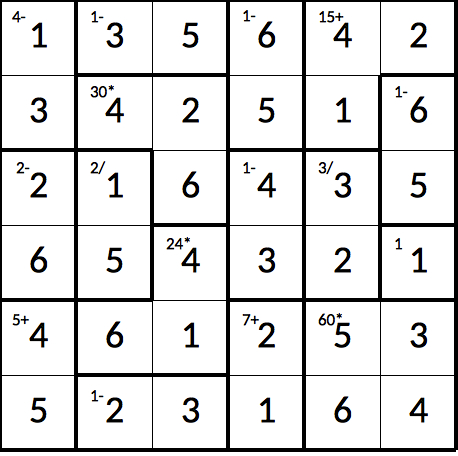
\includegraphics[scale=0.333]{Gambar/hybridgenetic/Generation1Chromosome1}
\caption[Kromosom 1 dalam Generasi ke-1]{Kromosom 1 dalam Generasi ke-1}
\label{fig:analisisg1k1}
\end{figure}

\item Gambar~\ref{fig:analisisg1k2} menggambarkan Kromosom 2.

\begin{figure}
\centering
\captionsetup{justification=centering}
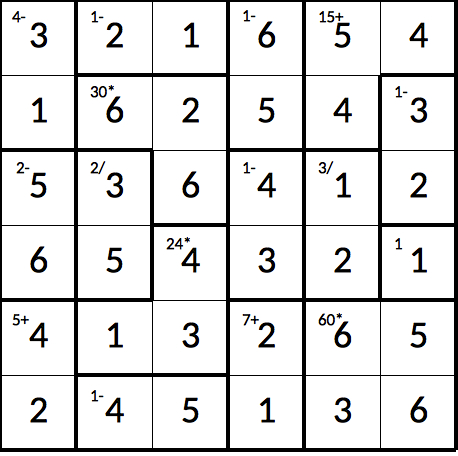
\includegraphics[scale=0.333]{Gambar/hybridgenetic/Generation1Chromosome2}
\caption[Kromosom 2 dalam Generasi ke-1]{Kromosom 2 dalam Generasi ke-1}
\label{fig:analisisg1k2}
\end{figure}

\item Gambar~\ref{fig:analisisg1k3} menggambarkan Kromosom 3.

\begin{figure}
\centering
\captionsetup{justification=centering}
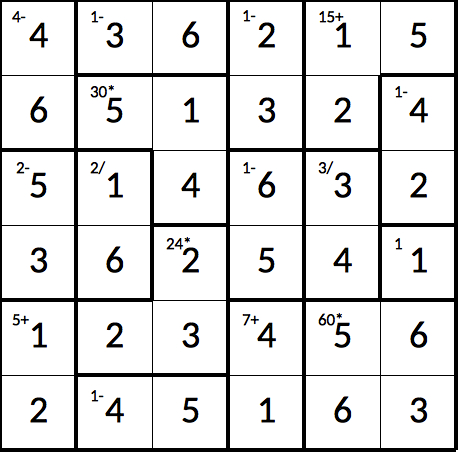
\includegraphics[scale=0.333]{Gambar/hybridgenetic/Generation1Chromosome3}
\caption[Kromosom 3 dalam Generasi ke-1]{Kromosom 3 dalam Generasi ke-1}
\label{fig:analisisg1k3}
\end{figure}


\item Gambar~\ref{fig:analisisg1k4} menggambarkan Kromosom 4.

\begin{figure}
\centering
\captionsetup{justification=centering}
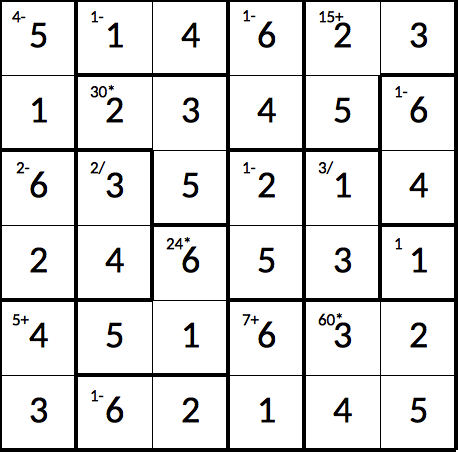
\includegraphics[scale=0.333]{Gambar/hybridgenetic/Generation1Chromosome4}
\caption[Kromosom 4 dalam Generasi ke-1]{Kromosom 4 dalam Generasi ke-1}
\label{fig:analisisg1k4}
\end{figure}

\item Gambar~\ref{fig:analisisg1k5} menggambarkan Kromosom 5.

\begin{figure}
\centering
\captionsetup{justification=centering}
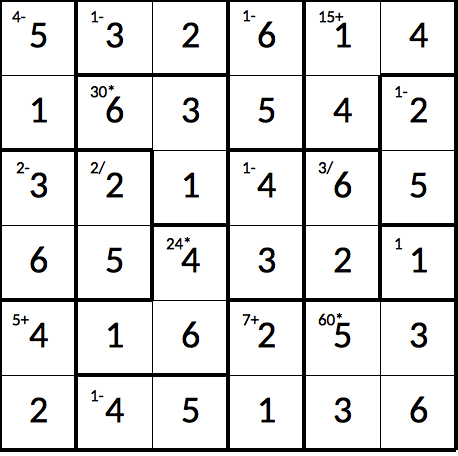
\includegraphics[scale=0.333]{Gambar/hybridgenetic/Generation1Chromosome5}
\caption[Kromosom 5 dalam Generasi ke-1]{Kromosom 5 dalam Generasi ke-1}
\label{fig:analisisg1k5}
\end{figure}

\item Gambar~\ref{fig:analisisg1k6} menggambarkan Kromosom 6.

\begin{figure}
\centering
\captionsetup{justification=centering}
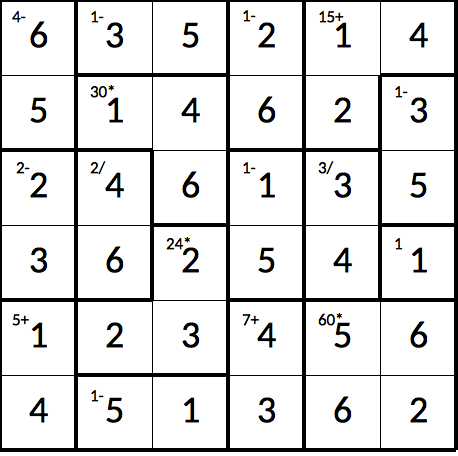
\includegraphics[scale=0.333]{Gambar/hybridgenetic/Generation1Chromosome6}
\caption[Kromosom 6 dalam Generasi ke-1]{Kromosom 6 dalam Generasi ke-1}
\label{fig:analisisg1k6}
\end{figure}

\item Gambar~\ref{fig:analisisg1k7} menggambarkan Kromosom 7.

\begin{figure}
\centering
\captionsetup{justification=centering}
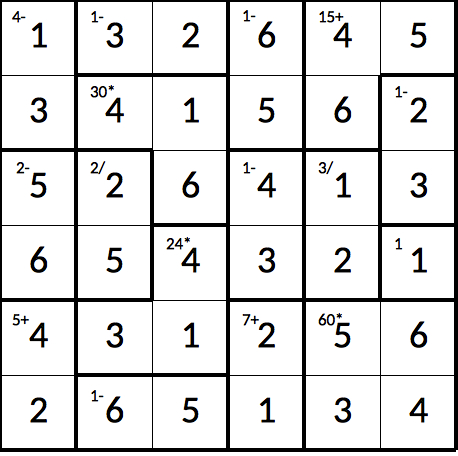
\includegraphics[scale=0.333]{Gambar/hybridgenetic/Generation1Chromosome7}
\caption[Kromosom 7 dalam Generasi ke-1]{Kromosom 7 dalam Generasi ke-1}
\label{fig:analisisg1k7}
\end{figure}

\item Gambar~\ref{fig:analisisg1k8} menggambarkan Kromosom 8.

\begin{figure}
\centering
\captionsetup{justification=centering}
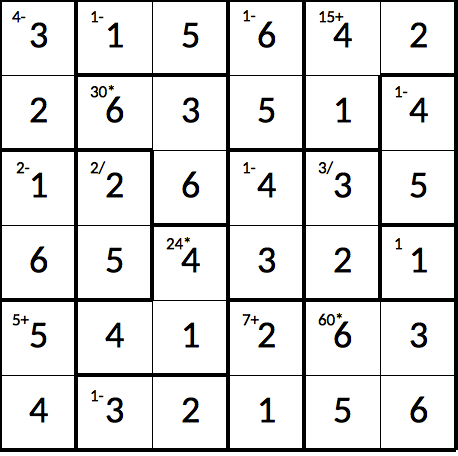
\includegraphics[scale=0.333]{Gambar/hybridgenetic/Generation1Chromosome8}
\caption[Kromosom 8 dalam Generasi ke-1]{Kromosom 8 dalam Generasi ke-1}
\label{fig:analisisg1k8}
\end{figure}

\item Gambar~\ref{fig:analisisg1k9} menggambarkan Kromosom 9.

\begin{figure}
\centering
\captionsetup{justification=centering}
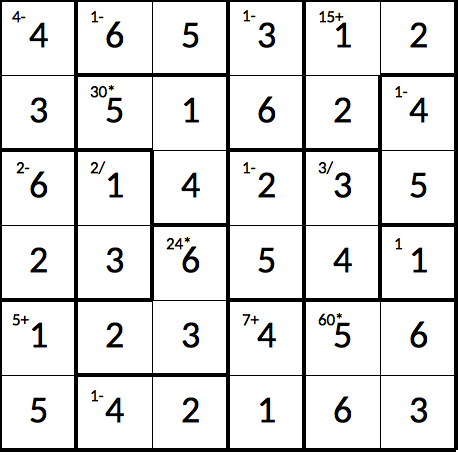
\includegraphics[scale=0.333]{Gambar/hybridgenetic/Generation1Chromosome9}
\caption[Kromosom 9 dalam Generasi ke-1]{Kromosom 9 dalam Generasi ke-1}
\label{fig:analisisg1k9}
\end{figure}

\item Gambar~\ref{fig:analisisg1k10} menggambarkan Kromosom 10.

\begin{figure}
\centering
\captionsetup{justification=centering}
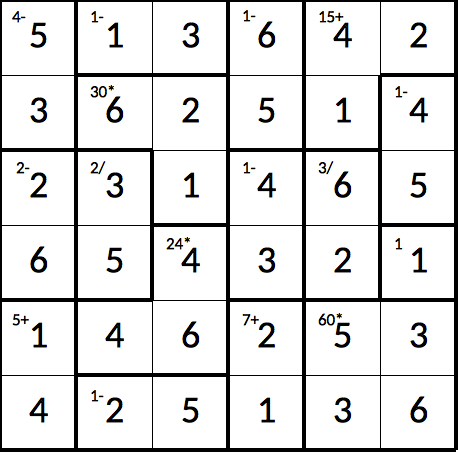
\includegraphics[scale=0.333]{Gambar/hybridgenetic/Generation1Chromosome10}
\caption[Kromosom 10 dalam Generasi ke-1]{Kromosom 10 dalam Generasi ke-1}
\label{fig:analisisg1k10}
\end{figure}

\item Gambar~\ref{fig:analisisg1k11} menggambarkan Kromosom 11.

\begin{figure}
\centering
\captionsetup{justification=centering}
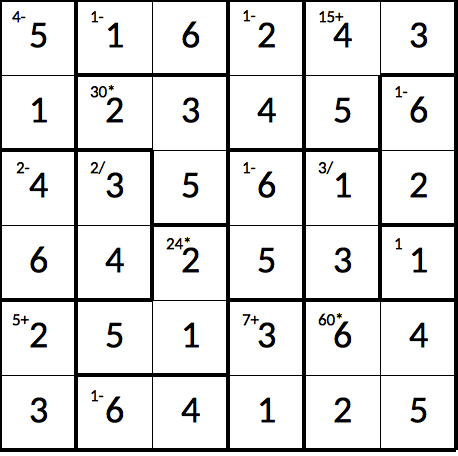
\includegraphics[scale=0.333]{Gambar/hybridgenetic/Generation1Chromosome11}
\caption[Kromosom 11 dalam Generasi ke-1]{Kromosom 11 dalam Generasi ke-1}
\label{fig:analisisg1k11}
\end{figure}

\item Gambar~\ref{fig:analisisg1k12} menggambarkan Kromosom 12.

\begin{figure}
\centering
\captionsetup{justification=centering}
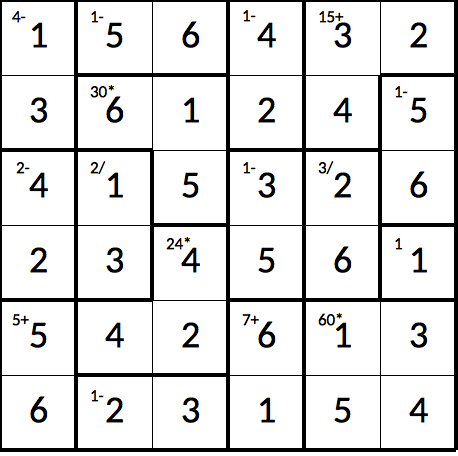
\includegraphics[scale=0.333]{Gambar/hybridgenetic/Generation1Chromosome12}
\caption[Kromosom 12 dalam Generasi ke-1]{Kromosom 12 dalam Generasi ke-1}
\label{fig:analisisg1k12}
\end{figure}

\end{enumerate}

Berdasarkan nilai kelayakan untuk kromosom-kromosom pada Generasi ke-1 yang ditampilkan pada Tabel~\ref{tab:analisishg2}, 5 kromosom terbaik akan diambil untuk menjadi bagian dari Generasi ke-2. Ke-5 kromosom yang terpilih adalah:
\begin{enumerate}
\item Kromosom 12
\item Kromosom 5
\item Kromosom 7
\item Kromosom 11
\item Kromosom 1
\end{enumerate}

\begin{table}
\centering
\captionsetup{justification=centering}
\caption[Tabel nilai kelayakan untuk kromosom-kromsom pada Generasi ke-1]{Tabel nilai kelayakan untuk kromosom-kromsom pada Generasi ke-1}
\begin{tabular}{| l | l |}
\hline
Nomor Kromosom & Nilai Kelayakan \\
\hline \hline
1 & 0,3333 \\
\hline
2 & 0,3056 \\
\hline
3 & 0,25 \\
\hline
4 & 0,2222 \\
\hline
5 & 0,4444 \\
\hline
6 & 0,1389 \\
\hline
7 & 0,3889 \\
\hline
8 & 0,25 \\
\hline
9 & 0,1389 \\
\hline
10 & 0,3056 \\
\hline
11 & 0,3889 \\
\hline
12 & 0,5556 \\
\hline
\end{tabular}
\label{tab:analisishg2}
\end{table}

Untuk Generasi ke-2, 5 kromosom adalah 5 kromosom terbaik dari Generasi ke-1, 6 kromosom adalah hasil kawin silang dari 2 kromosom dari Generasi ke-1, dan 1 kromosom adalah hasil mutasi dari 1 kromosom dari Generasi ke-1.

\begin{enumerate}
\item Gambar~\ref{fig:analisisg2k1} menggambarkan Kromosom 1, yaitu Kromosom 12 dari Generasi ke-1.

\begin{figure}
\centering
\captionsetup{justification=centering}
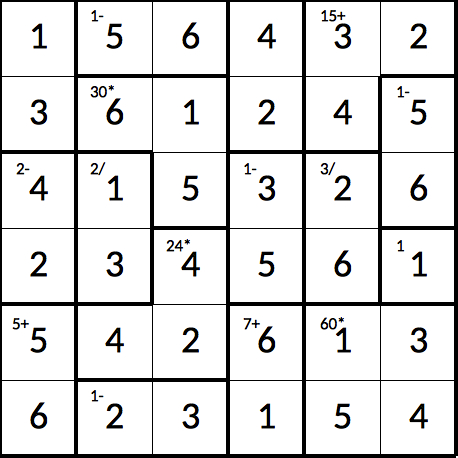
\includegraphics[scale=0.333]{Gambar/hybridgenetic/Generation2Chromosome1}
\caption[Kromosom 1 dalam Generasi ke-2]{Kromosom 1 dalam Generasi ke-2}
\label{fig:analisisg2k1}
\end{figure}


\item Gambar~\ref{fig:analisisg2k2} menggambarkan Kromosom 2, yaitu Kromosom 5 dari Generasi ke-1.

\begin{figure}
\centering
\captionsetup{justification=centering}
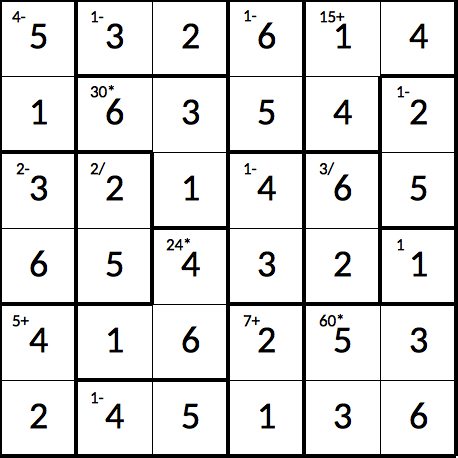
\includegraphics[scale=0.333]{Gambar/hybridgenetic/Generation2Chromosome2}
\caption[Kromosom 2 dalam Generasi ke-2]{Kromosom 2 dalam Generasi ke-2}
\label{fig:analisisg2k2}
\end{figure}

\item Gambar~\ref{fig:analisisg2k3} menggambarkan Kromosom 3, yaitu Kromosom 7 dari Generasi ke-1.

\begin{figure}
\centering
\captionsetup{justification=centering}
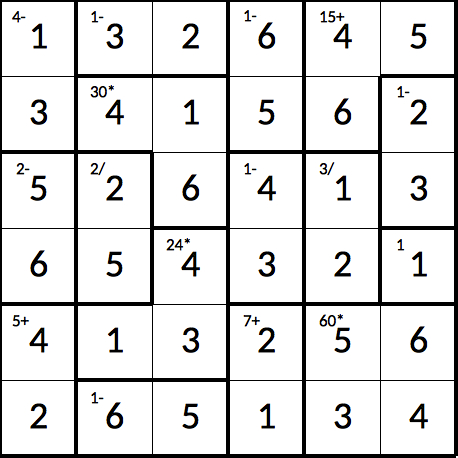
\includegraphics[scale=0.333]{Gambar/hybridgenetic/Generation2Chromosome3}
\caption[Kromosom 3 dalam Generasi ke-2]{Kromosom 3 dalam Generasi ke-2}
\label{fig:analisisg2k3}
\end{figure}

\item Gambar~\ref{fig:analisisg2k4} menggambarkan Kromosom 4, yaitu Kromosom 11 dari Generasi ke-1.

\begin{figure}
\centering
\captionsetup{justification=centering}
\includegraphics[scale=0.333]{Gambar/hybridgenetic/Generation2Chromosome4}
\caption[Kromosom 4 dalam Generasi ke-2]{Kromosom 4 dalam Generasi ke-2}
\label{fig:analisisg2k4}
\end{figure}

\item Gambar~\ref{fig:analisisg2k5} menggambarkan Kromosom 5, yaitu Kromosom 1 dari Generasi ke-1.

\begin{figure}
\centering
\captionsetup{justification=centering}
\includegraphics[scale=0.333]{Gambar/hybridgenetic/Generation2Chromosome5}
\caption[Kromosom 5 dalam Generasi ke-2]{Kromosom 5 dalam Generasi ke-2}
\label{fig:analisisg2k5}
\end{figure}

\item Gambar~\ref{fig:analisisg2k6} menggambarkan Kromosom 6, yaitu hasil kawin silang dari Kromosom 5 dan Kromosom 12 dari Generasi ke-1.

\begin{figure}
\centering
\captionsetup{justification=centering}
\includegraphics[scale=0.333]{Gambar/hybridgenetic/Generation2Chromosome6}
\caption[Kromosom 6 dalam Generasi ke-2]{Kromosom 6 dalam Generasi ke-2}
\label{fig:analisisg2k6}
\end{figure}

\item Gambar~\ref{fig:analisisg2k7} menggambarkan Kromosom 7, yaitu hasil kawin silang dari Kromosom 3 dan Kromosom 8 dari Generasi ke-1.

\begin{figure}
\centering
\captionsetup{justification=centering}
\includegraphics[scale=0.333]{Gambar/hybridgenetic/Generation2Chromosome7}
\caption[Kromosom 7 dalam Generasi ke-2]{Kromosom 7 dalam Generasi ke-2}
\label{fig:analisisg2k7}
\end{figure}

\item Gambar~\ref{fig:analisisg2k8} menggambarkan Kromosom 8, yaitu hasil kawin silang dari Kromosom 7 dan Kromosom 10 dari Generasi ke-1.

\begin{figure}
\centering
\captionsetup{justification=centering}
\includegraphics[scale=0.333]{Gambar/hybridgenetic/Generation2Chromosome8}
\caption[Kromosom 8 dalam Generasi ke-2]{Kromosom 8 dalam Generasi ke-2}
\label{fig:analisisg2k8}
\end{figure}

\item Gambar~\ref{fig:analisisg2k9} menggambarkan Kromosom 9, yaitu hasil kawin silang dari Kromosom 7 dan Kromosom 10 dari Generasi ke-1.

\begin{figure}
\centering
\captionsetup{justification=centering}
\includegraphics[scale=0.333]{Gambar/hybridgenetic/Generation2Chromosome9}
\caption[Kromosom 9 dalam Generasi ke-2]{Kromosom 9 dalam Generasi ke-2}
\label{fig:analisisg2k9}
\end{figure}

\item Gambar~\ref{fig:analisisg2k10} menggambarkan Kromosom 10, yaitu hasil kawin silang dari Kromosom 2 dan Kromosom 5 dari Generasi ke-1.

\begin{figure}
\centering
\captionsetup{justification=centering}
\includegraphics[scale=0.333]{Gambar/hybridgenetic/Generation2Chromosome10}
\caption[Kromosom 10 dalam Generasi ke-2]{Kromosom 10 dalam Generasi ke-2}
\label{fig:analisisg2k10}
\end{figure}

\item Gambar~\ref{fig:analisisg2k11} menggambarkan Kromosom 11, yaitu hasil kawin silang dari Kromosom 2 dan Kromosom 5 dari Generasi ke-1.

\begin{figure}
\centering
\captionsetup{justification=centering}
\includegraphics[scale=0.333]{Gambar/hybridgenetic/Generation2Chromosome11}
\caption[Kromosom 11 dalam Generasi ke-2]{Kromosom 11 dalam Generasi ke-2}
\label{fig:analisisg2k11}
\end{figure}

\item Gambar~\ref{fig:analisisg2k12} menggambarkan Kromosom 12, yaitu hasil mutasi dari Kromosom 12 dari Generasi ke-1.

\begin{figure}
\centering
\captionsetup{justification=centering}
\includegraphics[scale=0.333]{Gambar/hybridgenetic/Generation2Chromosome12}
\caption[Kromosom 12 dalam Generasi ke-2]{Kromosom 12 dalam Generasi ke-2}
\label{fig:analisisg2k12}
\end{figure}

\end{enumerate}

Berdasarkan nilai kelayakan untuk kromosom-kromosom pada Generasi ke-2 yang ditampilkan pada Tabel~\ref{tab:analisishg3}, 5 kromosom terbaik akan diambil untuk menjadi bagian dari Generasi ke-3. Ke-5 kromosom yang terpilih adalah:
\begin{enumerate}
\item Kromosom 1
\item Kromosom 12
\item Kromosom 2
\item Kromosom 3
\item Kromosom 4
\end{enumerate}

\begin{table}
\centering
\captionsetup{justification=centering}
\caption[Tabel nilai kelayakan untuk kromosom-kromsom pada Generasi ke-1]{Tabel nilai kelayakan untuk kromosom-kromsom pada Generasi ke-2}
\begin{tabular}{| l | l |}
\hline
Nomor Kromosom & Nilai Kelayakan \\
\hline \hline
1 & 0,5556 \\
\hline
2 & 0,4444 \\
\hline
3 & 0,3889 \\
\hline
4 & 0,3889 \\
\hline
5 & 0,3333 \\
\hline
6 & 0,1944 \\
\hline
7 & 0,1389 \\
\hline
8 & 0,0833 \\
\hline
9 & 0,25 \\
\hline
10 & 0,1944 \\
\hline
11 & 0,1944 \\
\hline
12 & 0,5 \\
\hline
\end{tabular}
\label{tab:analisishg3}
\end{table}

Untuk Generasi ke-3, 5 kromosom adalah 5 kromosom terbaik dari Generasi ke-2, 6 kromosom adalah hasil kawin silang dari 2 kromosom dari Generasi ke-2, dan 1 kromosom adalah hasil mutasi dari 1 kromosom dari Generasi ke-2.

\begin{enumerate}
\item Gambar~\ref{fig:analisisg3k1} menggambarkan Kromosom 1, yaitu Kromosom 1 dari Generasi ke-2.

\begin{figure}
\centering
\captionsetup{justification=centering}
\includegraphics[scale=0.333]{Gambar/hybridgenetic/Generation3Chromosome1}
\caption[Kromosom 1 dalam Generasi ke-3]{Kromosom 1 dalam Generasi ke-3}
\label{fig:analisisg3k1}
\end{figure}

\item Gambar~\ref{fig:analisisg3k2} menggambarkan Kromosom 2, yaitu Kromosom 12 dari Generasi ke-2.

\begin{figure}
\centering
\captionsetup{justification=centering}
\includegraphics[scale=0.333]{Gambar/hybridgenetic/Generation3Chromosome2}
\caption[Kromosom 2 dalam Generasi ke-3]{Kromosom 2 dalam Generasi ke-3}
\label{fig:analisisg3k2}
\end{figure}

\item Gambar~\ref{fig:analisisg3k3} menggambarkan Kromosom 3, yaitu Kromosom 2 dari Generasi ke-2.

\begin{figure}
\centering
\captionsetup{justification=centering}
\includegraphics[scale=0.333]{Gambar/hybridgenetic/Generation3Chromosome3}
\caption[Kromosom 3 dalam Generasi ke-3]{Kromosom 3 dalam Generasi ke-3}
\label{fig:analisisg3k3}
\end{figure}

\item Gambar~\ref{fig:analisisg3k4} menggambarkan Kromosom 4, yaitu Kromosom 3 dari Generasi ke-2.

\begin{figure}
\centering
\captionsetup{justification=centering}
\includegraphics[scale=0.333]{Gambar/hybridgenetic/Generation3Chromosome4}
\caption[Kromosom 4 dalam Generasi ke-3]{Kromosom 4 dalam Generasi ke-3}
\label{fig:analisisg3k4}
\end{figure}

\item Gambar~\ref{fig:analisisg3k5} menggambarkan Kromosom 5, yaitu Kromosom 4 dari Generasi ke-2.

\begin{figure}
\centering
\captionsetup{justification=centering}
\includegraphics[scale=0.333]{Gambar/hybridgenetic/Generation3Chromosome5}
\caption[Kromosom 5 dalam Generasi ke-3]{Kromosom 5 dalam Generasi ke-3}
\label{fig:analisisg3k5}
\end{figure}

\item Gambar~\ref{fig:analisisg3k6} menggambarkan Kromosom 6, yaitu hasil kawin silang dari Kromosom 2 dan Kromosom 12 dari Generasi ke-2.

\begin{figure}
\centering
\captionsetup{justification=centering}
\includegraphics[scale=0.333]{Gambar/hybridgenetic/Generation3Chromosome6}
\caption[Kromosom 6 dalam Generasi ke-3]{Kromosom 6 dalam Generasi ke-3}
\label{fig:analisisg3k6}
\end{figure}

\item Gambar~\ref{fig:analisisg3k7} menggambarkan Kromosom 7, yaitu hasil kawin silang dari Kromosom 2 dan Kromosom 12 dari Generasi ke-2.

\begin{figure}
\centering
\captionsetup{justification=centering}
\includegraphics[scale=0.333]{Gambar/hybridgenetic/Generation3Chromosome7}
\caption[Kromosom 7 dalam Generasi ke-3]{Kromosom 7 dalam Generasi ke-3}
\label{fig:analisisg3k7}
\end{figure}

\item Gambar~\ref{fig:analisisg3k8} menggambarkan Kromosom 8, yaitu hasil kawin silang dari Kromosom 5 dan Kromosom 9 dari Generasi ke-2.

\begin{figure}
\centering
\captionsetup{justification=centering}
\includegraphics[scale=0.333]{Gambar/hybridgenetic/Generation3Chromosome8}
\caption[Kromosom 8 dalam Generasi ke-3]{Kromosom 8 dalam Generasi ke-3}
\label{fig:analisisg3k8}
\end{figure}

\item Gambar~\ref{fig:analisisg3k9} menggambarkan Kromosom 9, yaitu hasil kawin silang dari Kromosom 5 dan Kromosom 9 dari Generasi ke-2.

\begin{figure}
\centering
\captionsetup{justification=centering}
\includegraphics[scale=0.333]{Gambar/hybridgenetic/Generation3Chromosome9}
\caption[Kromosom 9 dalam Generasi ke-3]{Kromosom 9 dalam Generasi ke-3}
\label{fig:analisisg3k9}
\end{figure}

\item Gambar~\ref{fig:analisisg3k10} menggambarkan Kromosom 10, yaitu hasil kawin silang dari Kromosom 5 dan Kromosom 6 dari Generasi ke-2.

\begin{figure}
\centering
\captionsetup{justification=centering}
\includegraphics[scale=0.333]{Gambar/hybridgenetic/Generation3Chromosome10}
\caption[Kromosom 10 dalam Generasi ke-3]{Kromosom 10 dalam Generasi ke-3}
\label{fig:analisisg3k10}
\end{figure}

\item Gambar~\ref{fig:analisisg3k11} menggambarkan Kromosom 11, yaitu hasil kawin silang dari Kromosom 5 dan Kromosom 6 dari Generasi ke-2.

\begin{figure}
\centering
\captionsetup{justification=centering}
\includegraphics[scale=0.333]{Gambar/hybridgenetic/Generation3Chromosome11}
\caption[Kromosom 11 dalam Generasi ke-3]{Kromosom 11 dalam Generasi ke-3}
\label{fig:analisisg3k11}
\end{figure}

\item Gambar~\ref{fig:analisisg3k12} menggambarkan Kromosom 12, yaitu hasil mutasi dari Kromosom 2 dari Generasi ke-2.

\begin{figure}
\centering
\captionsetup{justification=centering}
\includegraphics[scale=0.333]{Gambar/hybridgenetic/Generation3Chromosome12}
\caption[Kromosom 12 dalam Generasi ke-3]{Kromosom 12 dalam Generasi ke-3}
\label{fig:analisisg3k12}
\end{figure}

\end{enumerate}

\clearpage

Berdasarkan nilai kelayakan untuk kromosom-kromosom pada Generasi ke-3 yang ditampilkan pada Tabel~\ref{tab:analisishg4}, 5 kromosom terbaik akan diambil untuk menjadi bagian dari Generasi ke-4. Ke-5 kromosom yang terpilih adalah:
\begin{enumerate}
\item Kromosom 1
\item Kromosom 2
\item Kromosom 3
\item Kromosom 4
\item Kromosom 12
\end{enumerate}

\begin{table}
\centering
\captionsetup{justification=centering}
\caption[Tabel nilai kelayakan untuk kromosom-kromsom pada Generasi ke-3]{Tabel nilai kelayakan untuk kromosom-kromsom pada Generasi ke-3}
\begin{tabular}{| l | l |}
\hline
Nomor Kromosom & Nilai Kelayakan \\
\hline \hline
1 & 0,5556 \\
\hline
2 & 0,5 \\
\hline
3 & 0,4444 \\
\hline
4 & 0,3889 \\
\hline
5 & 0,3889 \\
\hline
6 & 0,2778 \\
\hline
7 & 0,1389 \\
\hline
8 & 0,1389 \\
\hline
9 & 0,1389 \\
\hline
10 & 0,1389 \\
\hline
11 & 0,1944 \\
\hline
12 & 0,3889 \\
\hline
\end{tabular}
\label{tab:analisishg4}
\end{table}

Proses ini diulang untuk menghasilkan generasi-generasi berikutnya, sampai algoritma genetik dapat menemukan solusi dari teka-teki Calcudoku tersebut.

\section{Analisis Perangkat Lunak}
\label{sec:analisispl}

Berdasarkan landasan teori dan analisis algoritma \textit{backtracking} dan \textit{hybrid genetic} untuk menyelesaikan permainan teka-teki Calcudoku yang telah dilakukan, perangkat lunak Calcudoku akan dibuat. Perangkat lunak ini akan menerima masukan dalam bentuk \textit{file} yang berisi:

\begin{enumerate}
\item Ukuran \textit{grid}.
\item Jumlah \textit{cage}.
\item Matriks \textit{cage assignment}, yang merepresentasikan posisi dari setiap \textit{cage} dalam \textit{grid}.
\item Matriks \textit{cage objectives}, yang berisikan angka tujuan dan operasi matematika yang telah ditentukan untuk setiap \textit{cage}.
\end{enumerate}

Umumnya, setiap soal hanya mempunyai satu solusi. Tetapi, ada juga soal yang tidak ada solusinya. Hal ini disebabkan karena kesalahan dalam merancang matriks \textit{cage assignment} dan matriks \textit{cage objectives}. Jika \textit{file} soal yang dibuka oleh perangkat lunak Calcudoku ternyata tidak ada solusinya, maka \textit{solver} akan selalu gagal dalam menyelesaikan permainan.

\clearpage

Perangkat lunak ini akan menghasilkan keluaran berupa antarmuka grafis permainan teka-teki Calcudoku berdasarkan isi \textit{file} yang di-\textit{load} oleh pengguna. Permainan ini dapat diselesaikan oleh pengguna dengan usahanya sendiri, atau menggunakan salah satu dari dua \textit{solver} yang disediakan.
Kedua \textit{solver} tersebut yaitu:

\begin{enumerate}
\item Algoritma \textit{backtracking}, dan
\item Algoritma \textit{hybrid genetic}.
\end{enumerate}

Pengguna dapat me-\textit{load} file masukan untuk memulai permainan, me-\textit{reset} permainan untuk mengulang permainan berdasarkan \textit{file} masukan yang sudah di-\textit{load} dari awal, dan menutup \textit{file} masukan untuk mengakhiri permainan, atau jika ingin me-\textit{load file} masukan yang lain. Pengguna juga dapat meminta perangkat lunak untuk memeriksa permainan jika ada masukan yang salah di dalam \textit{grid}, misalnya ada angka yang berulang dalam sebuah baris atau kolom, atau angka-angka dalam sebuah \textit{cage} tidak mencapai angka tujuan yang ditentukan setelah dihitung dengan operasi matematika yang ditentukan. Pemain juga dapat mengatur nilai dari parameter-parameter untuk algoritma genetik.

Kebutuhan-kebutuhan yang diperlukan oleh perangkat lunak ini akan dijelaskan menggunakan diagram \textit{use cage}, dan skenario.

\subsection{Diagram \textit{Use Case} dan Skenario}
\label{sec:analisisusecase}

Diagram \textit{use case} adalah diagram yang menggambarkan interaksi antara sistem (perangkat lunak) dengan pengguna. Berdasarkan analisis perangkat lunak yang telah dilakukan, maka pengguna dapat:

\begin{enumerate}
\item Membuka file masukan untuk memulai permainan.
\item Memilih salah satu dari dua \textit{solver} yang disediakan untuk menyelesaikan permainan berdasarkan \textit{file} yang sudah di-\textit{load}.
\item Me-\textit{reset} permainan untuk mengulang permainan berdasarkan \textit{file} masukan yang sudah di-\textit{load} dari awal.
\item Meminta perangkat lunak untuk memeriksa permainan jika ada masukan yang salah di dalam \textit{grid}.
\item Menutup \textit{file} masukan untuk mengakhiri permainan.
\item Menyelesaikan permainan dengan usahanya sendiri.
\item Mengatur nilai dari parameter-parameter untuk algoritma genetik.
\end{enumerate}

Diagram \textit{use case} untuk perangkat lunak permainan teka-teki Calcudoku dapat dilihat pada Gambar~\ref{fig:analisisusecase}.

\begin{figure}
\centering
\captionsetup{justification=centering}
\includegraphics[scale=0.5]{Gambar/Analisis/DiagramUseCase}
\caption[Diagram \textit{use case} untuk perangkat lunak permainan teka-teki Calcudoku]{Diagram \textit{use case} untuk perangkat lunak permainan teka-teki Calcudoku}
\label{fig:analisisusecase}
\end{figure}

Berdasarkan diagram \textit{use case} tersebut, skenario-skenario yang dapat dilakukan oleh pengguna adalah:

\begin{enumerate}
\item Membuka {file} masukan. Penjelasan untuk skenario ini dapat dilihat pada Tabel~\ref{tab:analisisload}.

\begin{table}
\centering
\captionsetup{justification=centering}
\caption[Skenario me-\textit{load file}]{Skenario me-\textit{load file}}
\begin{tabular}{| l || l |}
\hline
Nama & Membuka {file} masukan \\
\hline
Aktor & Pengguna \\
\hline
Deskripsi & Memembuka file masukan untuk memulai permainan. \\
\hline
Kondisi Awal & Perangkat lunak belum membuka {file} masukan. \\
\hline
Kondisi Akhir & Perangkat lunak sudah membuka {file} masukan .\\
\hline
Skenario Utama & \makecell[l]{Pengguna masuk ke dalam menu "\textit{File}", lalu memilih menu \textit{item} "\textit{Load} \\ \textit{Puzzle File}", lalu memilih \textit{file} masukan yang akan dibuka, dan mengklik \\ tombol "OK". Jika perangkat lunak sudah membuka {file} masukan, dan \\ ingin membuka {file} masukan yang baru, akan keluar kotak dialog "\textit{Are you} \\ \textit{sure you want to load another puzzle file}?", klik tombol "\textit{Yes}" untuk \\ membuka {file} masukan baru, atau klik tombol "\textit{No}" untuk membatalkan. \\ \textit{File} masukan yang akan dibuka harus \textit{file} teks.} \\
\hline
\end{tabular}
\label{tab:analisisload}
\end{table}

\item Memilih salah satu dari dua \textit{solver} yang disediakan. Penjelasan untuk skenario ini dapat dilihat pada Tabel~\ref{tab:analisischoose}

\begin{table}
\centering
\captionsetup{justification=centering}
\caption[Skenario memilih salah satu dari dua \textit{solver} yang disediakan]{Skenario memilih salah satu dari dua \textit{solver} yang disediakan}
\begin{tabular}{| l || l |}
\hline
Nama & Memilih salah satu dari dua \textit{solver} yang disediakan \\
\hline
Aktor & Pengguna \\
\hline
Deskripsi & \makecell[l]{Memilih salah satu dari dua \textit{solver} yang disediakan untuk menyelesaikan \\ permainan berdasarkan \textit{file} yang sudah di-\textit{load}.} \\
\hline
Kondisi Awal & \textit{Solver} belum menyelesaikan permainan. \\
\hline
Kondisi Akhir & \textit{Solver} berhasil atau gagal dalam menyelesaikan permainan. \\
\hline
Skenario Utama & \makecell[l]{Pengguna masuk ke dalam menu "\textit{Solve}", lalu memilih salah satu dari dua \\\textit{solver} yang disediakan. Pemain memilih menu \textit{item} "\textit{Backtracking}" untuk \\ memilih \textit{solver} dengan algoritma \textit{backtracking}, atau menu \textit{item} "\textit{Hybrid} \\ \textit{Genetic}" untuk memilih \textit{solver} dengan algoritma \textit{hybrid genetic}.} \\
\hline
\end{tabular}
\label{tab:analisischoose}
\end{table}

\item Me-\textit{reset} permainan. Penjelasan untuk skenario ini dapat dilihat pada Tabel~\ref{tab:analisisreset}.

\begin{table}
\centering
\captionsetup{justification=centering}
\caption[Skenario me-\textit{reset} permainan]{Skenario me-\textit{reset} permainan}
\begin{tabular}{| l || l |}
\hline
Nama & Me-\textit{reset} permainan \\
\hline
Aktor & Pengguna \\
\hline
Deskripsi & \makecell[l]{Me-\textit{reset} permainan untuk mengulang permainan berdasarkan \textit{file} masukan \\ yang sudah di-\textit{load} dari awal.} \\
\hline
Kondisi Awal & \makecell[l]{Permainan belum di-\textit{reset}, sel-sel dalam \textit{grid} mungkin masih berisi angka- \\ angka.} \\
\hline
Kondisi Akhir & \makecell[l]{Permainan sudah di-\textit{reset}, semua sel-sel dalam \textit{grid} sudah dalam keadaan \\ kosong.} \\
\hline
Skenario Utama & \makecell[l]{Pengguna masuk ke dalam menu "\textit{File}", lalu memilih menu \textit{item} "\textit{Reset} \\ \textit{Puzzle File}". Akan keluar kotak dialog "\textit{Are you sure you want to reset this} \\ \textit{puzzle?}", klik tombol "\textit{Yes} untuk me-\textit{reset} permainan, atau klik tombol \\ "\textit{No}" untuk membatalkan. Jika perangkat lunak belum me-\textit{load file} \\ masukan, maka akan keluar pesan \textit{error} "\textit{Puzzle file not loaded}".} \\
\hline
\end{tabular}
\label{tab:analisisreset}
\end{table}

\item Meminta perangkat lunak untuk memeriksa permainan. Penjelasan untuk skenario ini dapat dilihat pada Tabel~\ref{tab:analisischeck}.

\begin{table}
\centering
\captionsetup{justification=centering}
\caption[Skenario meminta perangkat lunak untuk memeriksa permainan]{Skenario meminta perangkat lunak untuk memeriksa permainan}
\begin{tabular}{| l || l |}
\hline
Nama & Meminta perangkat lunak untuk memeriksa permainan \\
\hline
Aktor & Pengguna \\
\hline
Deskripsi & \makecell[l]{Meminta perangkat lunak untuk memeriksa permainan jika ada masukan \\ yang salah di dalam \textit{grid}.} \\
\hline
Kondisi Awal & Permainan belum diperiksa oleh perangkat lunak. \\
\hline
Kondisi Akhir & \makecell[l]{Permainan sudah diperiksa oleh perangkat lunak. Pengguna akan \\ diberitahu oleh perangkat lunak jika ada masukan yang salah di dalam \\ \textit{grid}, misalnya ada angka yang berulang dalam sebuah baris atau kolom, \\ atau angka-angka dalam sebuah \textit{cage} tidak mencapai angka tujuan yang \\ ditentukan setelah dihitung dengan operasi matematika yang ditentukan.} \\
\hline
Skenario Utama & \makecell[l]{Pengguna masuk ke dalam menu "\textit{File}", lalu memilih menu \textit{item} "\textit{Check} \\ \textit{Puzzle File}". Jika perangkat lunak belum me-\textit{load file} masukan, maka akan \\ keluar pesan \textit{error} "\textit{Puzzle file not loaded}".} \\
\hline
\end{tabular}
\label{tab:analisischeck}
\end{table}

\item Menutup \textit{file} masukan. Penjelasan untuk skenario ini dapat dilihat pada Tabel~\ref{tab:analisisclose}.

\begin{table}
\centering
\captionsetup{justification=centering}
\caption[Skenario menutup \textit{file} masukan]{Skenario menutup \textit{file} masukan}
\begin{tabular}{| l || l |}
\hline
Nama & Menutup \textit{file} masukan \\
\hline
Aktor & Pengguna \\
\hline
Deskripsi & Menutup \textit{file} masukan untuk mengakhiri permainan. \\
\hline
Kondisi Awal & Perangkat lunak belum menutup \textit{file} masukan. \\
\hline
Kondisi Akhir & Perangkat lunak sudah menutup \textit{file} masukan. \\
\hline
Skenario Utama & \makecell[l]{Pengguna masuk ke dalam menu "\textit{File}", lalu memilih menu \textit{item} "\textit{Close} \\ \textit{Puzzle File}". Jika perangkat lunak belum me-\textit{load file} masukan, maka akan \\ keluar pesan \textit{error} "\textit{Puzzle file not loaded}".} \\
\hline
\end{tabular}
\label{tab:analisisclose}
\end{table}

\item Menyelesaikan permainan dengan usahanya sendiri. Penjelasan untuk skenario ini dapat dilihat pada Tabel~\ref{tab:analisisplay}.

\begin{table}
\centering
\captionsetup{justification=centering}
\caption[Skenario menyelesaikan permainan dengan usahanya sendiri]{Skenario menyelesaikan permainan dengan usahanya sendiri}
\begin{tabular}{| l || l |}
\hline
Nama & Menyelesaikan permainan dengan usahanya sendiri. \\
\hline
Aktor & Pengguna \\
\hline
Deskripsi & \makecell[l]{Pemain menyelesaikan permainan dengan usahanya sendiri. Pemain \\ mengisikan sel-sel dalam \textit{grid} dengan angka 1 sampai \begin{math}n\end{math}, dengan \begin{math}n\end{math} \\ merupakan ukuran dari \textit{grid}. Perangkat lunak dapat secara otomatis \\ memeriksa \textit{grid} jika ada masukan yang salah di dalam \textit{grid}, misalnya ada \\ angka yang berulang dalam sebuah baris atau kolom, atau angka-angka \\ dalam sebuah \textit{cage} tidak mencapai angka tujuan yang ditentukan setelah \\ dihitung dengan operasi matematika yang ditentukan.} \\
\hline
Kondisi Awal & Semua sel-sel dalam \textit{grid} dalam keadaan kosong. \\
\hline
Kondisi Akhir & \makecell[l]{Semua sel-sel dalam \textit{grid} sudah terisi dengan angka-angka, dengan rincian \\ tidak ada angka yang berulang dalam sebuah baris atau kolom, dan angka- \\ angka dalam setiap \textit{cage} mencapai angka tujuan yang ditentukan setelah \\ dihitung dengan operasi matematika yang ditentukan.} \\
\hline
Skenario Utama & \makecell[l]{Pemain mengisikan sel-sel dalam \textit{grid} dengan angka 1 sampai \begin{math}n\end{math}, dengan \begin{math}n\end{math} \\ merupakan ukuran dari \textit{grid}.} \\
\hline
\end{tabular}
\label{tab:analisisplay}
\end{table}

\item Mengatur nilai dari parameter-parameter untuk algoritma genetik. Penjelasan untuk skenario ini dapat dilihat pada Tabel~\ref{tab:analisissetparameters}.

\begin{table}
\centering
\captionsetup{justification=centering}
\caption[Skenario mengatur nilai dari parameter-parameter untuk algoritma genetik]{Skenario mengatur nilai dari parameter-parameter untuk algoritma genetik}
\begin{tabular}{| l || l |}
\hline
Nama & Mengatur nilai dari parameter-parameter untuk algoritma genetik \\
\hline
Aktor & Pengguna \\
\hline
Deskripsi & \makecell[l]{Pemain mengatur atau mengubah nilai dari parameter-parameter untuk \\ algoritma genetik dengan mengisi \textit{form} yang telah disediakan. Pemain \\ menekan tombol "OK" untuk mengatur atau mengubah nilai dari \\ parameter-parameter untuk algoritma genetik.} \\
\hline
Kondisi Awal & \makecell[l]{Parameter-parameter untuk algoritma genetik belum diatur, atau sudah \\ diatur tetapi belum diubah.} \\
\hline
Kondisi Akhir & \makecell[l]{Parameter-parameter untuk algoritma genetik sudah diatur jika belum \\ diatur sebelumnya, atau sudah diubah jadi sudah diatur sebelumnya.} \\
\hline
Skenario Utama & \makecell[l]{Pemain mengisikan \textit{form} yang telah disediakan, lalu menekan tombol \\ "OK". Nilai untuk parameter-parameter "\textit{Generations}" dan "\textit{Population} \\ \textit{Size}" harus bilangan bulat. Nilai untuk parameter-parameter "\textit{Elitism} \\ \textit{Rate}", "\textit{Crossover Rate}", dan "\textit{Mutation Rate}" harus bilangan desimal.}\\
\hline
\end{tabular}
\label{tab:analisissetparameters}
\end{table}

\end{enumerate}

\subsection{Diagram Kelas}
\label{sec:analisiskelas}

Berdasarkan diagram \textit{use case} yang telah dibuat, maka diagram kelas dapat dibuat. Diagram kelas untuk perangkat lunak permainan teka-teki Calcudoku dapat dilihat pada Gambar~\ref{fig:analisiskelas}.

\begin{figure}
\centering
\captionsetup{justification=centering}
\includegraphics[scale=0.5]{Gambar/Analisis/DiagramKelas.jpg}
\caption[Diagram kelas untuk perangkat lunak permainan teka-teki Calcudoku]{Diagram kelas untuk perangkat lunak permainan teka-teki Calcudoku}
\label{fig:analisiskelas}
\end{figure}

Berdasarkan diagram kelas tersebut, kelas-kelas yang digunakan dalam perangkat lunak Calcudoku adalah:

\begin{enumerate}
\item \textit{Package} model, yaitu \textit{package} yang berisi kelas-kelas yang merepresentasikan permainan teka-teki Calcudoku. \textit{Package} ini terdiri dari 8 kelas, yaitu:
	\begin{enumerate}
	\item Kelas Grid, yaitu kelas yang merepresentasikan sebuah \textit{grid} dalam permainan Calcudoku.
	\item Kelas Cell, yaitu kelas yang merepresentasikan sebuah sel dalam \textit{grid}.
	\item Kelas Cage, yaitu kelas yang merepresentasikan sebuah \textit{cage} dalam \textit{grid}.
	\item Kelas SolverBacktracking, yaitu kelas yang merepresentasikan \textit{solver} untuk permainan Calcudoku dengan algoritma \textit{backtracking}.
	\item Kelas SolverHybridGenetic, yaitu kelas yang merepresentasikan \textit{solver} untuk permainan Calcudoku dengan algoritma \textit{hybrid genetic}.
	\item Kelas SolverRuleBased, yaitu kelas yang merepresentasikan \textit{solver} untuk permainan Calcudoku dengan algoritma \textit{rule based}, bagian pertama dari algoritma \textit{hybrid genetic}.
	\item Kelas SolverGenetic, yaitu kelas yang merepresentasikan \textit{solver} untuk permainan Calcudoku dengan algoritma genetik, bagian kedua dari algoritma \textit{hybrid genetic}.
	\item Kelas Chromosome, yaitu kelas yang merepresentasikan sebuah kromosom dalam algoritma genetik.
	\end{enumerate}
\item \textit{Package} view, yaitu \textit{package} yang merepresentasikan GUI untuk permainan Calcudoku. \textit{Package} ini terdiri dari 2 kelas, yaitu:
	\begin{enumerate}
	\item Kelas Calcudoku, yaitu kelas yang merepresentasikan \textit{frame} untuk GUI permainan Calcudoku. Kelas ini berisi menu \textit{bar}, dan panel yang merepresentasikan \textit{grid} untuk permainan Calcudoku (kelas GUI).
	\item Kelas GUI, yaitu kelas yang merepresentasikan \textit{grid} untuk permainan Calcudoku.
	\item Kelas GeneticParameters, yaitu kelas yang berisi \textit{form} untuk mengatur nilai dari parameter-parameter untuk algoritma genetik.
	\end{enumerate}
\item \textit{Package} controller, yaitu penghubung antara kelas-kelas yang ada di dalam \textit{package} model dengan kelas-kelas yang ada di dalam \textit{package} view. \textit{Package} ini terdiri dari 1 kelas, yaitu kelas Controller. Kelas ini menghubungkan kelas-kelas yang ada di dalam \textit{package} model dengan kelas-kelas yang ada di dalam \textit{package} view.
\end{enumerate}

Penjelasan tentang variabel-variabel dan \textit{method-method} yang ada di dalam kelas-kelas di atas akan dijelaskan di dalam bab Perancangan.

\subsection{Diagram \textit{Sequence}}
\label{sec:diagramsequence}

Diagram \textit{sequence} adalah diagram yang menggambarkan interaksi antar kelas dalm suatu skenario. Diagram-diagram \textit{sequence} untuk perangkat lunak ini adalah sebagai berikut:

\begin{enumerate}

\item Gambar~\ref{fig:sequenceconstructor} menunjukkan diagram \textit{sequence} saat perangkat lunak dibuka.

\begin{figure}
\centering
\captionsetup{justification=centering}
\includegraphics[scale=0.5]{Gambar/Analisis/SequenceDiagramConstructor.png}
\caption[Diagram \textit{sequence} saat perangkat lunak dibuka]{Diagram \textit{sequence} saat perangkat lunak dibuka}
\label{fig:sequenceconstructor}
\end{figure}

\item Gambar~\ref{fig:sequenceload1} dan Gambar~\ref{fig:sequenceload2} menunjukkan diagram \textit{sequence} saat menu \textit{item} "\textit{Load Puzzle File}" dalam menu "\textit{File}" dipilih.

\begin{figure}
\centering
\captionsetup{justification=centering}
\includegraphics[scale=0.375]{Gambar/Analisis/SequenceDiagramLoad1.png}
\caption[Diagram \textit{sequence} saat menu \textit{item} "\textit{Load Puzzle File}" dalam menu "\textit{File}" dipilih (1)]{Diagram \textit{sequence} saat menu \textit{item} "\textit{Load Puzzle File}" dalam menu "\textit{File}" dipilih (1)}
\label{fig:sequenceload1}
\end{figure}

\begin{figure}
\centering
\captionsetup{justification=centering}
\includegraphics[scale=0.375]{Gambar/Analisis/SequenceDiagramLoad2.png}
\caption[Diagram \textit{sequence} saat menu \textit{item} "\textit{Load Puzzle File}" dalam menu "\textit{File}" dipilih (2)]{Diagram \textit{sequence} saat menu \textit{item} "\textit{Load Puzzle File}" dalam menu "\textit{File}" dipilih (2)}
\label{fig:sequenceload2}
\end{figure}

\item Gambar~\ref{fig:sequencefilechooser1} dan Gambar~\ref{fig:sequencefilechooser2} menunjukkan diagram \textit{sequence} saat \textit{file} permainan yang ingin dibuka dalam \textit{file chooser} dipilih.

\begin{figure}
\centering
\captionsetup{justification=centering}
\includegraphics[scale=0.375]{Gambar/Analisis/SequenceDiagramFileChooser1.png}
\caption[Diagram \textit{sequence} saat \textit{file} yang ingin dibuka dalam \textit{file chooser} dipilih (1)]{Diagram \textit{sequence} saat \textit{file} yang ingin dibuka dalam \textit{file chooser} dipilih (1)}
\label{fig:sequencefilechooser1}
\end{figure}

\begin{figure}
\centering
\captionsetup{justification=centering}
\includegraphics[scale=0.375]{Gambar/Analisis/SequenceDiagramFileChooser2.png}
\caption[Diagram \textit{sequence} saat \textit{file} yang ingin dibuka dalam \textit{file chooser} dipilih (2)]{Diagram \textit{sequence} saat \textit{file} yang ingin dibuka dalam \textit{file chooser} dipilih (2)}
\label{fig:sequencefilechooser2}
\end{figure}

\item Gambar~\ref{fig:sequenceloadpuzzlefile} menunjukkan diagram \textit{sequence} saat \textit{file} permainan yang sudah dipilih dibuka.

\begin{figure}
\centering
\captionsetup{justification=centering}
\includegraphics[scale=0.375]{Gambar/Analisis/SequenceDiagramLoadPuzzleFile.png}
\caption[Diagram \textit{sequence} saat \textit{file} permainan yang sudah dipilih dibuka]{Diagram \textit{sequence} saat \textit{file} permainan yang sudah dipilih dibuka}
\label{fig:sequenceloadpuzzlefile}
\end{figure}

\item Gambar~\ref{fig:sequencebt} menunjukkan diagram \textit{sequence} saat menu \textit{item} "\textit{Backtracking}" dalam menu "\textit{Solve}" dipilih.

\begin{figure}
\centering
\captionsetup{justification=centering}
\includegraphics[scale=0.375]{Gambar/Analisis/SequenceDiagramBacktracking.png}
\caption[Diagram \textit{sequence} saat menu \textit{item}" \textit{Backtracking}" dalam menu "\textit{Solve}" dipilih]{Diagram \textit{sequence} saat menu \textit{item}" \textit{Backtracking}" dalam menu "\textit{Solve}" dipilih}
\label{fig:sequencebt}
\end{figure}

\item Gambar~\ref{fig:sequencehg1} dan Gambar~\ref{fig:sequencehg2} menunjukkan diagram \textit{sequence} saat menu \textit{item} "\textit{Hybrid Genetic}" dalam menu "\textit{Solve}" dipilih.

\begin{figure}
\centering
\captionsetup{justification=centering}
\includegraphics[scale=0.333]{Gambar/Analisis/SequenceDiagramHybridGenetic1.png}
\caption[Diagram \textit{sequence} saat menu \textit{item} "\textit{Hybrid Genetic}" dalam menu "\textit{Solve}" dipilih (1)]{Diagram \textit{sequence} saat menu \textit{item} "\textit{Hybrid Genetic}" dalam menu "\textit{Solve}" dipilih (1)}
\label{fig:sequencehg1}
\end{figure}

\begin{figure}
\centering
\captionsetup{justification=centering}
\includegraphics[scale=0.333]{Gambar/Analisis/SequenceDiagramHybridGenetic2.png}
\caption[Diagram \textit{sequence} saat menu \textit{item} "\textit{Hybrid Genetic}" dalam menu "\textit{Solve}" dipilih (2)]{Diagram \textit{sequence} saat menu \textit{item} "\textit{Hybrid Genetic}" dalam menu "\textit{Solve}" dipilih (2)}
\label{fig:sequencehg2}
\end{figure}

\item Gambar~\ref{fig:sequencegaparameters} menunjukkan diagram \textit{sequence} saat menu \textit{item} "\textit{Set Genetic Algorithm Parameters}" dalam menu "\textit{Solve}" dipilih.

\begin{figure}
\centering
\captionsetup{justification=centering}
\includegraphics[scale=0.5]{Gambar/Analisis/SequenceDiagramGeneticParameters.png}
\caption[Diagram \textit{sequence} saat menu \textit{item}" \textit{Set Genetic Algorithm Parameters}" dalam menu "\textit{Solve}" dipilih]{Diagram \textit{sequence} saat menu \textit{item} "\textit{Set Genetic Algorithm Parameters}" dalam menu "\textit{Solve}" dipilih}
\label{fig:sequencegaparameters}
\end{figure}

\item Gambar~\ref{fig:sequencegaparametersok} menunjukkan diagram \textit{sequence} saat \textit{button} "\textit{OK}" dalam \textit{form} "\textit{Set Genetic Algorithm Parameters}" dalam menu "\textit{Solve}" dipilih.

\begin{figure}
\centering
\captionsetup{justification=centering}
\includegraphics[scale=0.5]{Gambar/Analisis/SequenceDiagramGeneticParametersOK.png}
\caption[Diagram \textit{sequence} saat \textit{button} "\textit{OK}" dalam \textit{form} "\textit{Set Genetic Algorithm Parameters}" dalam menu "\textit{Solve}" dipilih]{Diagram \textit{sequence} saat \textit{button} "\textit{OK}" dalam \textit{form} "\textit{Set Genetic Algorithm Parameters}" dalam menu "\textit{Solve}" dipilih}
\label{fig:sequencegaparametersok}
\end{figure}

\item Gambar~\ref{fig:sequencegaparameterscancel} menunjukkan diagram \textit{sequence} saat \textit{button} "\textit{Cancel}" dalam \textit{form} "\textit{Set Genetic Algorithm Parameters}" dalam menu "\textit{Solve}" dipilih.

\begin{figure}
\centering
\captionsetup{justification=centering}
\includegraphics[scale=0.5]{Gambar/Analisis/SequenceDiagramGeneticParametersCancel.png}
\caption[Diagram \textit{sequence} saat \textit{button} "\textit{Cancel}" dalam \textit{form} "\textit{Set Genetic Algorithm Parameters}" dalam menu "\textit{Solve}" dipilih]{Diagram \textit{sequence} saat \textit{button} "\textit{Cancel}" dalam \textit{form} "\textit{Set Genetic Algorithm Parameters}" dalam menu "\textit{Solve}" dipilih}
\label{fig:sequencegaparameterscancel}
\end{figure}

\item Gambar~\ref{fig:sequencecheck} menunjukkan diagram \textit{sequence} saat menu \textit{item} "\textit{Check Puzzle File}" dalam menu "\textit{File}" dipilih.

\begin{figure}
\centering
\captionsetup{justification=centering}
\includegraphics[scale=0.5]{Gambar/Analisis/SequenceDiagramCheck.png}
\caption[Diagram \textit{sequence} saat menu \textit{item} "\textit{Check Puzzle File}" dalam menu "\textit{File}" dipilih]{Diagram \textit{sequence} saat menu \textit{item} "\textit{Check Puzzle File}" dalam menu "\textit{File}" dipilih}
\label{fig:sequencecheck}
\end{figure}

\item Gambar~\ref{fig:sequencereset} menunjukkan diagram \textit{sequence} saat menu \textit{item} "\textit{Reset Puzzle}" dalam menu "\textit{File}" dipilih.

\begin{figure}
\centering
\captionsetup{justification=centering}
\includegraphics[scale=0.375]{Gambar/Analisis/SequenceDiagramReset.png}
\caption[Diagram \textit{sequence} saat menu \textit{item} "\textit{Reset Puzzle}" dalam menu "\textit{File}" dipilih]{Diagram \textit{sequence} saat menu \textit{item} "\textit{Reset Puzzle}" dalam menu "\textit{File}" dipilih}
\label{fig:sequencereset}
\end{figure}

\item Gambar~\ref{fig:sequenceclose} menunjukkan diagram \textit{sequence} saat menu \textit{item} "\textit{Close Puzzle File}" dalam menu "\textit{File}" dipilih.

\begin{figure}
\centering
\captionsetup{justification=centering}
\includegraphics[scale=0.5]{Gambar/Analisis/SequenceDiagramClose.png}
\caption[Diagram \textit{sequence} saat menu \textit{item} "\textit{Close Puzzle File}" dalam menu "\textit{File}" dipilih]{Diagram \textit{sequence} saat menu \textit{item} "\textit{Close Puzzle File}" dalam menu "\textit{File}" dipilih}
\label{fig:sequenceclose}
\end{figure}

\item Gambar~\ref{fig:sequenceexit} menunjukkan diagram \textit{sequence} saat perangkat lunak ditutup.

\begin{figure}
\centering
\captionsetup{justification=centering}
\includegraphics[scale=0.5]{Gambar/Analisis/SequenceDiagramExit.png}
\caption[Diagram \textit{sequence} saat perangkat lunak ditutup]{Diagram \textit{sequence} saat perangkat lunak ditutup}
\label{fig:sequenceexit}
\end{figure}

\end{enumerate}}{}
\ifdefstring{\vbabd}{1}{\chapter{Perancangan}
\label{chap:perancangan}

Bab ini membahas tentang perancangan perangkat lunak yang dibuat. Bab ini juga akan membahas tentang perancangan masukan, perancangan keluaran, diagram kelas, diagram \textit{use case}, diagram aktivitas, dan diagram \textit{sequence} untuk perangkat lunak tersebut.

\section{Perancangan Masukan}
\label{sec:perancanganmasukan}

Masukan untuk perangkat lunak permainan teka-teki Calcudoku ini berupa sebuah \textit{file} teks, seperti yang ditunjukkan pada Gambar~\ref{fig:perancanganmasukan}.

\begin{figure}
\centering
\captionsetup{justification=centering}
\includegraphics[scale=0.5]{Gambar/Perancangan/PerancanganInput.png}
\caption[Contoh \textit{file} masukan.]{Contoh \textit{file} masukan.}
\label{fig:perancanganmasukan}
\end{figure}

Adapun rincian dari \textit{file text} masukan tersebut adalah sebagai berikut:

\begin{enumerate}
\item Baris pertama berisi ukuran \textit{grid} dan banyaknya \textit{cage} dari teka-teki Calcudoku tersebut. Angka pertama adalah ukuran \textit{grid}, dan angka kedua adalah banyaknya \textit{cage}.
\item Baris kedua sampai ke baris ke-\begin{math}2 + (n - 1)\end{math}, dengan \begin{math}n\end{math} adalah ukuran \textit{grid}, berisi matriks \textit{cage assignment}. Matriks ini merepresentasikan posisi dari setiap \textit{cage} dalam \textit{grid}. Setiap \textit{cage} direpresentasikan dengan angka yang berbeda. Setiap \textit{cage} dapat mempunyai ukuran (jumlah sel yang terdapat dalam \textit{cage}) yang bervariasi. Setiap sel dalam sebuah \textit{cage} harus berhubungan secara horizontal atau vertikal dengan sel lain dalam \textit{cage} yang sama.
\item Baris ke-\begin{math}2 + n\end{math} dan seterusnya berisi \textit{cage objectives} untuk setiap \textit{cage}. \textit{Cage objectives} berisikan angka tujuan dan operasi matematika yang telah ditentukan. Angka-angka dalam sebuah \textit{cage} harus mencapai angka tujuan jika dihitung menggunakan operasi matematika yang telah ditentukan.
\end{enumerate}

\section{Perancangan Keluaran}
\label{sec:perancangankeluaran}

Keluaran untuk perangkat lunak permainan teka-teki Calcudoku ini berupa sebuah matriks yang berisi solusi dari teka-teki Calcudoku yang sudah diselesaikan oleh program, seperti dapat dilihat pada Gambar~\ref{fig:perancangankeluaran}.

\begin{figure}
\centering
\captionsetup{justification=centering}
\includegraphics[scale=1]{Gambar/Perancangan/PerancanganOutput.png}
\caption[Contoh keluaran.]{Contoh keluaran.}
\label{fig:perancangankeluaran}
\end{figure}


\section{Diagram Kelas}
\label{sec:diagramkelas}

Perangkat lunak teka-teki Calcudoku ini terdiri dari beberapa kelas, yang dikelompokkan dalam tiga package, yaitu:

\begin{enumerate}
\item Model, yaitu \textit{engine} dari perangkat lunak ini. Package ini memiliki beberapa kelas, yaitu:
	\begin{enumerate}
	\item Grid, yaitu kelas yang merepresentasikan \textit{grid} dalam teka-teki Calcudoku.
	\item Cell, yaitu kelas yang merepresentasikan sel dalam teka-teki Calcudoku.
	\item Cage, yaitu kelas yang merepresentasikan \textit{cage} dalam teka-teki Calcudoku.
	\item SolverBacktracking, yaitu kelas \textit{solver} untuk teka-teki Calcudoku menggunakan algoritma backtracking.
	\item SolverHybridGenetic, yaitu kelas \textit{solver} untuk teka-teki Calcudoku menggunakan algoritma \textit{hybrid genetic}. Algoritma ini akan mencoba menyelesaikan teka-teki Calcudoku menggunakan algoritma \textit{rule based} terlebih dahulu. Algoritma genetik baru akan dijalankan jika algoritma \textit{rule based} gagal dalam menyelesaikan teka-teki Calcudoku.
	\item SolverRuleBased, yaitu kelas \textit{solver} untuk teka-teki Calcudoku menggunakan algoritma \textit{rule based}. Dalam algoritma \textit{hybrid genetic}, algoritma akan mencoba menyelesaikan teka-teki Calcudoku menggunakan algoritma \textit{rule based} terlebih dahulu.
	\item SolverGenetic, yaitu kelas \textit{solver} untuk teka-teki Calcudoku menggunakan algoritma genetik. Dalam algoritma \textit{hybrid genetic}, algoritma genetik baru akan dijalankan jika algoritma \textit{rule based} gagal dalam menyelesaikan teka-teki Calcudoku.
	\item Chromosome, yaitu kelas yang merepresentasikan sebuah kromosom untuk algoritma genetik dalam solver \textit{hybrid genetic}.
	\item ChromosomeComparator, yaitu kelas pembanding \textit{custom} (\textit{custom comparator}) yang berfungsi untuk mengurutkan kromosom berdasarkan nilai kelayakkannya (\textit{fitness value}).	
	\item SolverGenetic, yaitu kelas \textit{solver} untuk teka-teki Calcudoku menggunakan algoritma genetik. Dalam algoritma \textit{hybrid genetic}, algoritma genetik baru akan dijalankan jika algoritma \textit{rule based} gagal dalam menyelesaikan teka-teki Calcudoku.
	\end{enumerate}
\item View, yaitu GUI dari perangkat lunak ini. Package ini memiliki beberapa kelas, yaitu:
	\begin{enumerate}
	\item Calcudoku, yaitu kelas \textit{frame} yang berisi menu \textit{bar} dan instansiasi kelas panel GUI.
	\item WindowListener, yaitu kelas \textit{listener} untuk kelas Calcudoku. \textit{Listener} ini berfungsi untuk menambahkan pesan peringatan saat akan menutup perangkat lunak.
	\item PuzzleFileFilter, yaitu kelas filter untuk \textit{file chooser}. Filter ini membatasi agar \textit{file chooser} hanya bisa membuka \textit{file} teks.
	\item GUI, yaitu kelas panel yang merepresentasikan GUI dari permainan teka-teki Calcudoku.
	\item CellKeyListener, yaitu kelas \textit{listener} untuk kelas GUI. \textit{Listener} ini berfungsi untuk menggerakkan kursor dari sebuah sel ke sel di sebelahnya menggunakan tombol-tombol panah ke kiri, ke atas, ke bawah, dan ke kanan. Listener ini juga berfungsi untuk membatasi agar sel hanya bisa diisi oleh satu angka.
	\item PopupMenuListener, yaitu kelas \textit{listener} untuk kelas GUI. \textit{Listener} ini berfungsi untuk mengisi sel dengan angka menggunakan menu \textit{pop up}, sel akan diisi dengan angka yang dipilih.
	\item CellTextFieldListener, yaitu kelas \textit{listener} untuk kelas GUI. \textit{Listener} ini berfungsi untuk mengisikan sel dalam kelas Grid dengan angka yang diisikan ke dalam sel dalam GUI.
	\end{enumerate}
\item Controller, yaitu penghubung antara \textit{package} model dan \textit{package} view. Package ini hanya berisi satu kelas, yaitu kelas Controller.
\end{enumerate}

Diagram kelas untuk perangkat lunak ini dapat dilihat pada Gambar~\ref{fig:diagramkelas}.

\begin{figure}
\centering
\captionsetup{justification=centering}
\includegraphics[scale=0.2]{Gambar/Perancangan/DiagramKelas.jpg}
\caption[Diagram kelas untuk perangkat lunak Calcudoku.]{Diagram kelas untuk perangkat lunak Calcudoku.}
\label{fig:diagramkelas}
\end{figure}

Berikut ini adalah rincian dari setiap kelas, dengan setiap atribut dan setiap \textit{method} yang dimilikinya.

\subsection{Kelas Grid}
\label{sec:kelasgrid}

Kelas Grid mempunyai beberapa atribut, yaitu:

\begin{enumerate}
\item size, yaitu ukuran dari matriks \textit{grid}.
\item numberOfCages, yaitu banyaknya \textit{cage} yang terdapat dalam \textit{grid}.
\item cageCells, yaitu sebuah matriks \textit{cage assignment}. Matriks ini merepresentasikan posisi dari setiap \textit{cage} dalam \textit{grid}.
\item cageObjectives, yaitu sebuah \textit{array} yang berisi \textit{cage objectives} untuk setiap \textit{cage}. \textit{Cage objectives} berisikan angka tujuan dan operasi matematika yang telah ditentukan.
\item grid, yaitu representasi dari \textit{grid} dalam teka-teki Calcudoku. grid adalah sebuah matriks yang berisi sel-sel. Matriks ini berukuran \begin{math} n \times n\end{math}.
\item cages, yaitu representasi dari sebuah \textit{cage} dalam sebuah \textit{grid}.
\end{enumerate}

Kelas Grid mempunyai beberapa \textit{method}, yaitu:

\begin{enumerate}
\item Grid(Integer size, Integer numberOfCages, Integer[][] cageCells, String[] cageObjectives), yaitu konstruktor dari kelas ini. Konstruktor ini menerima masukan berupa ukuran dari matriks \textit{grid}, banyaknya \textit{cage} yang terdapat dalam \textit{grid}, matriks \textit{cage assignment}, dan array \textit{cage objectives}.
\item countAreas(Integer[][] array), yaitu \textit{method} pembungkus dari \textit{method} countAreas(int[][] array, boolean[][] checked). \textit{Method} ini menerima masukan berupa array \textit{cage assignment} untuk sebuah \textit{cage}, dan menghasilkan keluaran berupa jumlah area dari \textit{cage} tersebut.
\item countAreas(Integer[][] array, boolean[][] checked), yaitu \textit{method} yang menghitung jumlah area dari sebuah \textit{cage} secara rekursif dengan menggunakan algoritma \textit{flood fill}. \textit{Method} ini menerima masukan berupa array \textit{cage assignment} untuk sebuah \textit{cage} dan sebuah array checked yang berfungsi untuk menandai sel-sel yang sudah pernah dikunjungi atau belum, dan menghasilkan keluaran berupa jumlah area dari \textit{cage} tersebut.
\item floodFill(int i, int j, Integer[][] array, boolean[][] checked), yaitu implementasi dari algoritma \textit{flood fill} untuk menghitung jumlah area dari sebuah \textit{cage}. \textit{Method} ini menerima masukan berupa posisi baris dan kolom dari sebuah sel, array \textit{cage assignment} untuk sebuah \textit{cage} dan sebuah array checked yang berfungsi untuk menandai sel-sel yang sudah pernah dikunjungi atau belum.
\item isCageCellsSizeValid(Integer[][] cageCells), yaitu \textit{method} yang memeriksa apakah ukuran matriks \textit{cage assignment} valid atau tidak. \textit{Method} ini menerima masukan berupa matriks \textit{cage assignment}, dan menghasilkan keluaran apakah matriks tersebut \textit{valid} atau tidak. Matriks tersebut \textit{valid} jika ukuran barisnya dan kolomnya sama dengan variabel size.
\item isCageObjectivesSizeValid(String[] cageObjectives), yaitu \textit{method} yang memeriksa apakah ukuran matriks \textit{cage objectives} valid atau tidak. \textit{Method} ini menerima masukan berupa \textit{array cage objectives}, dan menghasilkan keluaran apakah \textit{array} tersebut \textit{valid} atau tidak. Array tersebut \textit{valid} jika ukuran dari \textit{array} tersebut sama dengan variabel numberOfCages.
\item isCageAssignmentValid(Integer[][] array), yaitu \textit{method} yang memeriksa apakah \textit{cage assignment} untuk sebuah \textit{cage valid} atau tidak. \textit{Method} ini menerima masukan berupa matriks \textit{cage assignment} untuk sebuah \textit{cage} dan menghasilkan keluaran apakah matriks tersebut atau tidak. Matriks tersebut \textit{valid} jika jumlah area dari \textit{cage} tersebut adalah satu.
\item isCagesValid(Cage[] cages), yaitu \textit{method} yang memeriksa apakah setiap \textit{cage} yang ada di dalam \textit{grid valid} atau tidak. \textit{Method} ini menerima masukan berupa \textit{array cage}, dan menghasilkan keluaran apakah \textit{array} tersebut \textit{valid} atau tidak. \textit{Array} tersebut \textit{valid} jika setiap \textit{cage} dengan operator = hanya berukuran satu sel, setiap \textit{cage} dengan operator + atau \begin{math}\times\end{math} berukuran minimal dua sel, dan setiap \textit{cage} dengan operator - atau \begin{math}\div\end{math} berukuran tepat dua sel.
\item generateCages(Cage[] cages), yaitu \textit{method} yang membangkitkan \textit{cage-cage} dalam sebuah \textit{grid}. \textit{Method} ini menerima masukan berupa sebuah array \textit{Cage} yang kosong.
\item generateGrid(Cell[][] grid, Cage[] cages), yaitu \textit{method} yang membangkitkan \textit{grid} dan \textit{cage assignment} dari \textit{grid} tersebut.. \textit{Method} ini menerima masukan berupa sebuah matriks sel yang kosong dan sebuah array \textit{cage} yang kosong.
\item getRow(int rowNumber), yaitu \textit{method} untuk mendapatkan isi dari sebuah baris yang diminta. \textit{Method} ini menerima masukan berupa nomor baris yang diminta dan menghasilkan keluaran berupa isi baris yang diminta.
\item getColumn(int columnNumber), yaitu \textit{method} untuk mendapatkan isi dari sebuah kolom yang diminta. \textit{Method} ini menerima masukan berupa nomor kolom yang diminta dan menghasilkan keluaran berupa isi kolom yang diminta dalam bentuk ArrayList.
\item getCageValues(int cageNumber), yaitu \textit{method} untuk mendapatkan isi dari sebuah \textit{cage} yang diminta. \textit{Method} ini menerima masukan berupa nomor \textit{cage} yang diminta dan menghasilkan keluaran berupa isi \textit{cage} yang diminta dalam bentuk ArrayList.
\item isArrayValid(ArrayList<Integer> array), yaitu \textit{method} untuk memeriksa apakah sebuah \textit{array valid} atau tidak. \textit{Method} ini menerima masukan berupa \textit{array} yang akan diperiksa dan menghasilkan keluaran apakah \textit{array} tersebut \textit{valid} atau tidak. \textit{Array} tersebut \textit{valid} jika tidak ada angka yang berulang dalam \textit{array} tersebut.
\item isRowValid(int row), yaitu \textit{method} untuk memeriksa apakah sebuah baris \textit{valid} atau tidak. \textit{Method} ini menerima masukan berupa nomor baris yang diminta dan menghasilkan keluaran apakah baris yang diminta tersebut \textit{valid} atau tidak. Baris tersebut \textit{valid} jika tidak ada angka yang berulang dalam baris tersebut.
\item solverIsRowValid(int column), yaitu \textit{method} yang sama dengan isRowValid, tetapi \textit{method} ini hanya untuk dipanggil oleh solver.
\item isColumnValid(int column), yaitu \textit{method} untuk memeriksa apakah sebuah kolom \textit{valid} atau tidak. \textit{Method} ini menerima masukan berupa nomor kolom yang diminta dan menghasilkan keluaran apakah kolom yang diminta tersebut \textit{valid} atau tidak. Kolom tersebut \textit{valid} jika tidak ada angka yang berulang dalam kolom tersebut.
\item solverIsColumnValid(int column), yaitu \textit{method} yang sama dengan isColumnValid, tetapi \textit{method} ini hanya untuk dipanggil oleh solver.
\item isCageValuesValid(int cageNumber), yaitu \textit{method} untuk memeriksa apakah nilai dari setiap sel yang berada dalam sebuah \textit{cage valid} atau tidak. \textit{Method} ini menerima masukan berupa nomor \textit{cage} yang diminta dan menghasilkan keluaran apakah nilai dari setiap sel yang berada dalam \textit{cage} yang diminta tersebut \textit{valid} atau tidak. \textit{Cage} tersebut \textit{valid} jika nilai dari setiap sel yang berada di dalam \textit{cage} tersebut mencapai angka tujuan yang telah ditentukan jika dihitung menggunakan operator yang telah ditentukan.
\item isCageValid(int row, int column), yaitu \textit{method} untuk memeriksa apakah sebuah \textit{cage valid} atau tidak. \textit{Method} ini menerima masukan berupa nomor baris dan nomor kolom dari sebuah sel yang diminta dan menghasilkan keluaran apakah \textit{cage} yang berisi sel tersebut \textit{valid} atau tidak. \textit{Cage} tersebut \textit{valid} jika angka-angka dalam \textit{cage} tersebut mencapai angka tujuan yang telah ditentukan jika dihitung menggunakan operator yang telah ditentukan.
\item solverIsCageValid(int column), yaitu \textit{method} yang sama dengan isCageValid, tetapi \textit{method} ini hanya untuk dipanggil oleh solver.
\item isCellValueValid(int row, int column), yaitu \textit{method} untuk memeriksa apakah nilai dari sel tersebut \textit{valid} atau tidak. \textit{Method} ini menerima masukan berupa nomor baris dan nomor kolom dari sel yang akan diperiksa dan menghasilkan keluaran apakah nilai dari sel tersebut \textit{valid} atau tidak. Nilai dari sebuah sel \textit{valid} jika nilai dari sel tersebut tidak berulang dalam baris dan kolom tempat sel tersebut berada, dan angka-angka dari \textit{cage} yang berisi sel tersebut mencapai angka tujuan yang telah ditentukan jika dihitung menggunakan operator yang telah ditentukan.
\item solverIsCellValueValid(int column), yaitu \textit{method} yang sama dengan isCellValueValid, tetapi \textit{method} ini hanya untuk dipanggil oleh solver.
\item setCellValue(int row, int column, Integer value), yaitu \textit{method} untuk mengisi sebuah sel dengan nilai yang telah ditentukan. \textit{Method} ini menerima masukan berupa nomor baris dan nomor kolom dari sel yang akan diisi dan nilai dari sel tersebut, dan menghasilkan keluaran apakah nilai dari sel tersebut \textit{valid} atau tidak. Nilai dari sebuah sel \textit{valid} jika nilai dari sel tersebut tidak berulang dalam baris dan kolom tempat sel tersebut berada, dan angka-angka dari \textit{cage} yang berisi sel tersebut mencapai angka tujuan yang telah ditentukan jika dihitung menggunakan operator yang telah ditentukan.
\item solverSetCellValue(int row, int column, Integer value), yaitu \textit{method} yang sama dengan setCellValue, tetapi \textit{method} ini hanya untuk dipanggil oleh solver.
\item unsetCellValue(int row, int column), yaitu \textit{method} untuk menghapus isi dari sebuah sel. \textit{Method} ini menerima masukan berupa nomor baris dan nomor kolom dari sel yang akan dihapus isinya.
\item isWin(), yaitu \textit{method} yang memeriksa apakah semua sel sudah diisi dengan nilai yang \textit{valid} atau tidak. \textit{Method} ini menghasilkan keluaran apakah semua sel sudah diisi dengan nilai yang \textit{valid} atau tidak. \textit{Method} ini menghasilkan \textit{null} jika ada sel yang belum diisi.
\item checkGrid(), yaitu \textit{method} yang memeriksa apakah ada sel yang berisi nilai yang tidak \textit{valid} atau tidak. \textit{Method} ini akan menghasilkan apakah ada sel yang berisi nilai yang tidak \textit{valid} atau tidak. \textit{Method} ini hanya bekerja jika semua sel yang berada di dalam \textit{grid} sudah diisi. Nilai dari sebuah sel \textit{valid} jika nilai dari sel tersebut tidak berulang dalam baris dan kolom tempat sel tersebut berada, dan angka-angka dari \textit{cage} yang berisi sel tersebut mencapai angka tujuan yang telah ditentukan jika dihitung menggunakan operator yang telah ditentukan.
\item isFilled(), yaitu \textit{method} yang memeriksa apakah semua sel sudah diisi atau tidak. \textit{Method} ini menghasilkan keluaran apakah semua sel sudah diisi atau tidak.
\item getCellValue(int row, int column), yaitu \textit{method} untuk mendapatkan isi dari sebuah sel. \textit{Method} ini menerima masukan berupa nomor baris dan nomor kolom dari sel yang diminta dan menghasilkan keluaran berupa isi dari sel yang diminta tersebut.
\item getSize(), yaitu \textit{method} untuk mendapatkan ukuran dari \textit{grid}. \textit{Method} ini menghasilkan keluaran berupa ukuran dari \textit{grid}.
\item getNumberOfCages(), yaitu \textit{method} untuk mendapatkan jumlah \textit{cage} yang ada di dalam \textit{grid}. \textit{Method} ini menghasilkan keluaran berupa jumlah \textit{cage} yang ada di dalam \textit{grid}.
\item getCageCells(), yaitu \textit{method} untuk mendapatkan matriks \textit{cage assignment} dari \textit{grid}. \textit{Method} ini menghasilkan keluaran berupa matriks \textit{cage assignment} dari \textit{grid}.
\item getCageObjectives(), yaitu \textit{method} untuk mendapatkan \textit{cage objectives} dari setiap \textit{cage} dalam \textit{grid}. \textit{Method} ini menghasilkan keluaran berupa sebuah array yang berisi \textit{cage objectives} dari setiap \textit{cage} dalam \textit{grid}.
\item getGridContents(), yaitu \textit{method} untuk mendapatkan nilai dari setiap sel \textit{grid}. \textit{Method} ini menghasilkan keluaran berupa sebuah matriks yang berisi nilai dari setiap sel \textit{grid}.
\item getCages(), yaitu \textit{method} untuk mendapatkan semua \textit{cage} dalam \textit{grid}. \textit{Method} ini menghasilkan keluaran berupa array yang berisi semua \textit{cage} dalam \textit{grid}.
\item getGame(), yaitu \textit{method} untuk mendapatkan instansiasi saat ini dari kelas \textit{Grid}. \textit{Method} ini menghasilkan keluara berupa instansiasi saat ini dari kelas \textit{Grid}.
\end{enumerate}

Diagram kelas Grid dapat dilihat pada Gambar~\ref{fig:diagramkelasgrid}.

\begin{figure}
\centering
\captionsetup{justification=centering}
\includegraphics[scale=0.5]{Gambar/Perancangan/DiagramKelasGrid.png}
\caption[Diagram kelas Grid.]{Diagram kelas Grid.}
\label{fig:diagramkelasgrid}
\end{figure}

\subsection{Kelas Cage}
\label{sec:kelascage}

Kelas Cage mempunyai beberapa atribut, yaitu:

\begin{enumerate}
\item cageID, yaitu nomor dari \textit{cage} tersebut.
\item objective, yaitu angka tujuan dan operator yang ditentukan untuk \textit{cage} tersebut.
\item targetNumber, yaitu angka tujuan dari \textit{cage} tersebut.
\item operator, yaitu operator yang ditentukan untuk \textit{cage} tersebut.
\item cells, yaitu sebuah array yang berisi sel-sel yang merupakan anggota dari \textit{cage} tersebut.
\end{enumerate}

Kelas Cage mempunyai \textit{method-method} berikut:

\begin{enumerate}
\item Cage(int cageID, String objectives), yaitu konstruktor dari kelas ini. Konstruktor ini menerima masukan berupa nomor dan \textit{cage objectives} dari \textit{cage} tersebut.
\item isCageObjectiveValid(String cageObjective), yaitu \textit{method} yang memeriksa apakah \textit{cage objective} dari \textit{cage} tersebut \textit{valid} atau tidak. \textit{Method} ini menerima masukan berupa String yang berisi \textit{cage objective} dan menghasilkan keluaran apakah String tersebut valid atau tidak. \textit{Cage objective valid} jika isi dari \textit{cage objective} tersebut adalah satu angka tujuan dari \textit{cage} tersebut dan diikuti oleh satu operator yang telah ditentukan untuk \textit{cage} tersebut.
\item generateTargetNumber(String objective), yaitu \textit{method} yang membangkitkan angka tujuan dari sebuah \textit{cage} dari \textit{cage objective} yang diberikan. \textit{Method} ini menerima masukan berupa String yang berisi \textit{cage objective} dari sebuah \textit{cage} dan menghasilkan keluaran berupa angka tujuan dari \textit{cage} tersebut.
\item generateOperator(String objective), yaitu \textit{method} yang membangkitkan operator yang telah ditentukan untuk sebuah \textit{cage} dari \textit{cage objective} yang diberikan. \textit{Method} ini menerima masukan berupa String yang berisi \textit{cage objective} dari sebuah \textit{cage} dan menghasilkan keluaran berupa operator yang telah ditentukan untuk \textit{cage} tersebut.
\item addCell(Cell c), yaitu \textit{method} untuk menambahkan sebuah sel kedalam sebuah \textit{cage}. \textit{Method} ini menerima masukan berupa sel yang akan dimasukkan ke dalam \textit{cage}.
\item isCageContainsNull(), yaitu \textit{method} yang memeriksa apakah sebuah \textit{cage} mempunyai sel yang belum diisi. \textit{Method} ini menghasilkan keluaran apakah \textit{cage} tersebut mempunyai sel yang belum terisi.
\item isCageValuesValid(), yaitu \textit{method} yang memeriksa apakah angka-angka dalam sebuah \textit{cage} mencapai angka tujuan dari \textit{cage} tersebut jika dihitung menggunakan operator yang telah ditentukan untuk \textit{cage} tersebut. \textit{Method} ini menghasilkan keluaran apakah angka-angka dalam \textit{cage} tersebut mencapai angka tujuan dari \textit{cage} tersebut jika dihitung menggunakan operator yang telah ditentukan untuk \textit{cage} tersebut. \textit{Method} ini menghasilkan \textit{null} jika ada sel di dalam \textit{cage} yang belum diisi.
\item countValue(), yaitu \textit{method} yang menghitung angka-angka di dalam sebuah \textit{cage} menggunakan operator yang telah ditentukan untuk \textit{cage} tersebut. \textit{Method} ini menghasilkan keluaran hasil perhitungan dari angka-angka di dalam sebuah \textit{cage} menggunakan operator yang telah ditentukan untuk \textit{cage} tersebut. \textit{Method} ini menghasilkan \textit{null} jika ada sel di dalam \textit{cage} yang belum diisi.
\item getTargetNumber(), yaitu \textit{method} untuk mendapatkan angka tujuan dari sebuah \textit{cage}. \textit{Method} ini menghasilkan keluaran berupa angka tujuan dari \textit{cage} tersebut.
\item getOperator(), yaitu \textit{method} untuk mendapatkan operator yang telah ditentukan untuk sebuah \textit{cage}. \textit{Method} ini menghasilkan keluaran berupa operator yang telah ditentukan untuk \textit{cage} tersebut.
\item getCells(), yaitu \textit{method} untuk mendapatkan sel-sel anggota sebuah \textit{cage}. \textit{Method} ini menghasilkan keluaran sebuah ArrayList yang berisi sel-sel anggota \textit{cage} tersebut.
\item getSize(), yaitu \textit{method} untuk mendapatkan jumlah dari sel-sel anggota sebuah \textit{cage}. \textit{Method} ini menghasilkan keluaran berupa jumlah dari sel-sel anggota \textit{cage} tersebut.
\end{enumerate}

Diagram kelas Cage dapat dilihat pada Gambar~\ref{fig:diagramkelascage}.

\begin{figure}
\centering
\captionsetup{justification=centering}
\includegraphics[scale=0.5]{Gambar/Perancangan/DiagramKelasCage.png}
\caption[Diagram kelas Cage.]{Diagram kelas Cage.}
\label{fig:diagramkelascage}
\end{figure}

\subsection{Kelas Cell}
\label{sec:kelascell}

Kelas Cell mempunyai beberapa atribut, yaitu:

\begin{enumerate}
\item cellID, yaitu nomor dari sel tersebut.
\item row, yaitu posisi baris dari sel tersebut.
\item column, yaitu posisi kolom dari sel tersebut.
\item cageID, yaitu nomor \textit{cage} yang berisi sel tersebut.
\item value, yaitu nilai dari sel tersebut.
\end{enumerate}

Kelas Cell mempunyai beberapa \textit{method}, yaitu:

\begin{enumerate}
\item Cell(int CellID, int row, int column, int cageID), yaitu konstruktor dari kelas ini. Konstruktor ini menerima masukan berupa nomor sel, nomor baris, dan nomor kolom dari sel tersebut, dan nomor \textit{cage} yang berisi sel tersebut.
\item setValue(Integer value), yaitu \textit{method} untuk mengisi sebuah sel tersebut dengan nilai yang telah ditentukan. \textit{Method} ini menerima masukan berupa nilai yang akan diisikan ke dalam sel tersebut.
\item getValue(), yaitu \textit{method} untuk mendapatkan nilai dari sel tersebut. \textit{Method} ini menghasilkan keluaran berupa nilai dari sel tersebut.
\item getRow(), yaitu \textit{method} untuk mendapatkan nomor baris dari sebuah sel. \textit{Method} ini menghasilkan keluaran berupa nomor baris dari sel tersebut.
\item getColumn(), yaitu \textit{method} untuk mendapatkan nomor kolom dari sebuah sel. \textit{Method} ini menghasilkan keluaran berupa nomor kolom dari sel tersebut.
\item getCageID(), yaitu \textit{method} untuk mendapatkan nomor \textit{cage} yang berisi sebuah sel. \textit{Method} ini menghasilkan keluaran berupa nomor \textit{cage} yang berisi sel tersebut.
\end{enumerate}

Diagram kelas Cell dapat dilihat pada Gambar~\ref{fig:diagramkelascell}.

\begin{figure}
\centering
\captionsetup{justification=centering}
\includegraphics[scale=0.5]{Gambar/Perancangan/DiagramKelasCell.png}
\caption[Diagram kelas Cell.]{Diagram kelas Cell.}
\label{fig:diagramkelascell}
\end{figure}

\subsection{Kelas SolverBacktracking}
\label{sec:kelassolverbt}

Kelas SolverBacktracking mempunyai beberapa atribut, yaitu:

\begin{enumerate}
\item grid, yaitu \textit{grid} yang akan diselesaikan oleh \textit{solver} dengan algoritma \textit{backtracking}.
\item size, yaitu ukuran dari \textit{grid} yang akan diselesaikan oleh \textit{solver} dengan algoritma \textit{backtracking}.
\item solution, yaitu \textit{grid} yang sudah diselesaikan oleh \textit{solver} dengan algoritma \textit{backtracking}.
\end{enumerate}

Kelas SolverBacktracking mempunyai beberapa \textit{method}, yaitu:

\begin{enumerate}
\item SolverBacktracking(Grid grid), yaitu konstruktor dari kelas ini. Konstruktor ini menerima masukan berupa \textit{grid} yang akan diselesaikan oleh \textit{solver} dengan algoritma \textit{backtracking}.
\item solve(), yaitu \textit{method} pembungkus dari \textit{method} solve(int row, int column). \textit{Method} ini menghasilkan keluaran apakah \textit{solver} berhasil menyelesaikan teka-teki Calcudoku atau tidak. \textit{Solver} bekerja mulai dari sel pada sudut kiri atas, lalu bergerak ke kanan sampai ke sel yang paling kanan, lalu bergerak ke baris berikutnya sampai ke baris yang paling bawah, selesai pada sel pada sudut kanan bawah.
\item solve(int row, int column), yaitu \textit{method} yang mencoba untuk menyelesaikan teka-teki Calcudoku menggunakan algoritma \textit{backtracking}. \textit{Method} ini menerima masukan berupa nomor baris dan nomor kolom yang akan diisi oleh \textit{solver} dan menghasilkan keluaran apakah nilai yang diisi oleh \textit{solver valid} atau tidak. \textit{Solver} akan mulai mengisi sel dari angka 1. Jika berhasil, maka \textit{solver} akan maju ke sel berikutnya. Jika gagal, maka \textit{solver} akan mencoba kemungkinan angka berikutnya. Jika semua kemungkinan angka gagal, maka \textit{solver} akan mundur ke sel sebelumnya dan mencoba kemungkinan angka berikutnya.
\item getGrid(), yaitu \textit{method} untuk mendapatkan \textit{grid}. \textit{Method} ini menghasilkan keluaran berupa \textit{grid}.
\item getSolution(), yaitu \textit{method} untuk mendapatkan solusi dari \textit{grid} yang sudah diselesaikan oleh \textit{solver}. \textit{Method} ini menghasilkan keluaran berupa solusi dari \textit{grid} tersebut.
\item printGrid(), yaitu \textit{method} untuk mencetak isi \textit{grid} ke layar.
\end{enumerate}

Diagram kelas SolverBacktracking dapat dilihat pada Gambar~\ref{fig:diagramkelassolverbt}.

\begin{figure}
\centering
\captionsetup{justification=centering}
\includegraphics[scale=0.5]{Gambar/Perancangan/DiagramKelasSolverBacktracking.png}
\caption[Diagram kelas SolverBacktracking.]{Diagram kelas SolverBacktracking.}
\label{fig:diagramkelassolverbt}
\end{figure}

\subsection{Kelas SolverHybridGenetic}
\label{sec:kelassolverhg}

Kelas SolverHybridGenetic mempunyai beberapa atribut, yaitu:

\begin{enumerate}
\item grid, yaitu \textit{grid} yang akan diselesaikan oleh \textit{solver} dengan algoritma \textit{hybrid genetic}.
\item gridRuleBased, yaitu \textit{grid} yang telah diselesaikan oleh algoritma \textit{rule based}.
\item size, yaitu ukuran dari \textit{grid} yang akan diselesaikan oleh \textit{solver} dengan algoritma \textit{hybrid genetic}.
\item solution, yaitu \textit{grid} yang sudah diselesaikan oleh \textit{solver} dengan algoritma \textit{hybrid genetic}.
\end{enumerate}

Kelas SolverHybridGenetic mempunyai beberapa \textit{method}, yaitu:

\begin{enumerate}
\item SolverHybridGenetic(Grid grid), yaitu konstruktor dari kelas ini. Konstruktor ini menerima masukan berupa \textit{grid} yang akan diselesaikan oleh \textit{solver} dengan algoritma \textit{hybrid genetic}.
\item solve(), yaitu \textit{method} yang mencoba untuk menyelesaikan teka-teki Calcudoku menggunakan algoritma \textit{hybrid genetic}. \textit{Method} ini akan memanggil solver algoritma \textit{rule based}. Jika algoritma \textit{rule based} gagal dalam menyelesaikan teka-teki Calcudoku, maka \textit{method} akan memanggil solver algoritma genetik. \textit{Method} ini menghasilkan keluaran apakah \textit{solver} berhasil menyelesaikan teka-teki Calcudoku atau tidak.
\item printGrid(), yaitu \textit{method} untuk mencetak isi \textit{grid} ke layar.
\end{enumerate}

Diagram kelas SolverHybridGenetic dapat dilihat pada Gambar~\ref{fig:diagramkelassolverhg}.

\begin{figure}
\centering
\captionsetup{justification=centering}
\includegraphics[scale=0.5]{Gambar/Perancangan/DiagramKelasSolverHybridGenetic.png}
\caption[Diagram kelas SolverHybridGenetic.]{Diagram kelas SolverHybridGenetic.}
\label{fig:diagramkelassolverhg}
\end{figure}

\subsection{Kelas SolverRuleBased}
\label{sec:kelassolverrb}

Kelas SolverRuleBased mempunyai beberapa atribut, yaitu:

\begin{enumerate}
\item grid, yaitu \textit{grid} yang akan diselesaikan oleh \textit{solver} dengan algoritma \textit{rule based}.
\item size, yaitu ukuran dari \textit{grid} yang akan diselesaikan oleh \textit{solver} dengan algoritma \textit{rule based}.
\item solution, yaitu \textit{grid} yang sudah diselesaikan oleh \textit{solver} dengan algoritma \textit{rule based}.
\item possibleValues, yaitu sebuah \textit{array} yang menampung semua kemungkinan angka yang mungkin untuk setiap sel yang ada di dalam \textit{grid}
\end{enumerate}

Kelas SolverRuleBased mempunyai \textit{method-method} berikut:

\begin{enumerate}
\item SolverRuleBased(Grid grid), yaitu konstruktor dari kelas ini. Konstruktor ini menerima masukan berupa \textit{grid} yang akan diselesaikan oleh \textit{solver} dengan algoritma \textit{rule based}.
\item generatePossibleValuesArray(), yaitu \textit{method} yang membangkitkan kemungkinan angka-angka yang mungkin untuk setiap sel yang ada di dalam \textit{grid}. Angka-angka yang mungkin adalah dari 1 sampai ke ukuran dari \textit{grid}. \textit{Method} ini menghasilkan keluaran berupa array yang menampung semua kemungkinan angka yang mungkin untuk setiap sel yang ada di dalam \textit{grid}.
\item solve(), yaitu \textit{method} yang mencoba untuk menyelesaikan teka-teki Calcudoku menggunakan algoritma \textit{rule based}. \textit{Method} ini menghasilkan keluaran apakah \textit{solver} berhasil menyelesaikan teka-teki Calcudoku atau tidak. \textit{Solver} akan mencoba menyelesaikan teka-teki Calcudoku menggunakan aturan-aturan logika, misalnya \textit{single square rule}, \textit{killer combination rule}, \textit{naked subset rule}, \textit{hidden subset rule}, dan \textit{evil twin rule}. Aturan \textit{single square} dan \textit{killer combination} hanya dipakai sekali, dan dilakukan oleh \textit{method} ini, sedangkan aturan \textit{naked subset}, \textit{hidden subset}, dan \textit{evil twin} dapat dipakai berkali-kali, dan dilakukan oleh \textit{method} solveLoop().
\item solveLoop(), yaitu \textit{method} yang mengaplikasikan aturan \textit{naked subset}, \textit{hidden subset}, dan \textit{evil twin} kepada \textit{grid} yang sedang diselesaikan oleh algoritma \textit{rule based}. \textit{Method} ini menerima masukan berupa \textit{array} kemungkinan angka yang mungkin untuk setiap sel yang ada di dalam \textit{grid}. \textit{Method} ini akan diulang sampai \textit{method} ini tidak bisa mengisi sel-sel yang ada di dalam \textit{grid}.
\item getRowPossibleValues(int rowNumber), yaitu \textit{method} untuk mendapatkan kemungkinan angka-angka yang mungkin dari sel-sel yang ada di dalam baris yang diminta. \textit{Method} ini menerima masukan berupa nomor baris yang diminta dan menghasilkan keluaran berupa kemungkinan angka-angka yang mungkin dari sel-sel yang ada di dalam baris yang diminta.
\item getColumnPossibleValues(int rowNumber), yaitu \textit{method} untuk mendapatkan kemungkinan angka-angka yang mungkin dari sel-sel yang ada di dalam kolom yang diminta. \textit{Method} ini menerima masukan berupa nomor kolom yang diminta dan menghasilkan keluaran berupa kemungkinan angka-angka yang mungkin dari sel-sel yang ada di dalam kolom yang diminta.
\item singleSquare(), yaitu \textit{method} yang mengaplikasikan aturan \textit{single square} kepada \textit{grid} yang sedang diselesaikan oleh algoritma \textit{rule based}.
\item killerCombination(), yaitu \textit{method} yang mengaplikasikan aturan \textit{killer combination} kepada \textit{grid} yang sedang diselesaikan oleh algoritma \textit{rule based}. Dalam perangkat lunak ini aturan ini dibatasi hanya untuk \textit{cage} yang berukuran dua sel.
\item killerCombinationCageSize2(), yaitu \textit{method} yang mengaplikasikan aturan \textit{killer combination} kepada setiap \textit{cage} yang berukuran 2 di dalam \textit{grid} yang sedang diselesaikan oleh algoritma \textit{rule based}.
\item killerCombinationCageSize2GridSize3(), yaitu \textit{method} yang mengaplikasikan aturan \textit{killer combination} kepada setiap \textit{cage} yang berukuran 2 sel di dalam \textit{grid} yang berukuran \begin{math}3 \times 3\end{math} yang sedang diselesaikan oleh algoritma \textit{rule based}.
\item killerCombinationCageSize2GridSize4(), yaitu \textit{method} yang mengaplikasikan aturan \textit{killer combination} kepada setiap \textit{cage} yang berukuran 2 sel di dalam \textit{grid} yang berukuran \begin{math}4 \times 4\end{math} yang sedang diselesaikan oleh algoritma \textit{rule based}.
\item killerCombinationCageSize2GridSize5(), yaitu \textit{method} yang mengaplikasikan aturan \textit{killer combination} kepada setiap \textit{cage} yang berukuran 2 sel di dalam \textit{grid} yang berukuran \begin{math}5 \times 5\end{math} yang sedang diselesaikan oleh algoritma \textit{rule based}.
\item killerCombinationCageSize2GridSize6(), yaitu \textit{method} yang mengaplikasikan aturan \textit{killer combination} kepada setiap \textit{cage} yang berukuran 2 sel di dalam \textit{grid} yang berukuran \begin{math}6 \times 6\end{math} yang sedang diselesaikan oleh algoritma \textit{rule based}.
\item killerCombinationCageSize2GridSize7(), yaitu \textit{method} yang mengaplikasikan aturan \textit{killer combination} kepada setiap \textit{cage} yang berukuran 2 sel di dalam \textit{grid} yang berukuran \begin{math}7 \times 7\end{math} yang sedang diselesaikan oleh algoritma \textit{rule based}.
\item killerCombinationCageSize2GridSize8(), yaitu \textit{method} yang mengaplikasikan aturan \textit{killer combination} kepada setiap \textit{cage} yang berukuran 2 sel di dalam \textit{grid} yang berukuran \begin{math}8 \times 8\end{math} yang sedang diselesaikan oleh algoritma \textit{rule based}.
\item killerCombinationCageSize2GridSize9(), yaitu \textit{method} yang mengaplikasikan aturan \textit{killer combination} kepada setiap \textit{cage} yang berukuran 2 sel di dalam \textit{grid} yang berukuran \begin{math}9 \times 9\end{math} yang sedang diselesaikan oleh algoritma \textit{rule based}.
\item evilTwin(), yaitu \textit{method} yang mengaplikasikan aturan \textit{evil twin} kepada \textit{grid} yang sedang diselesaikan oleh algoritma \textit{rule based}. Dalam perangkat lunak ini aturan ini dibatasi hanya untuk \textit{cage} dengan operator + dan \begin{math}\times\end{math}.
\item evilTwin(int cageID), yaitu \textit{method} yang mengaplikasikan aturan \textit{evil twin} kepada sebuah \textit{cage} di dalam \textit{grid} yang sedang diselesaikan oleh algoritma \textit{rule based}. \textit{Method} ini menerima masukan berupa nomor \textit{grid} yang akan diaplikasikan dengan aturan \textit{evil twin}.
\item nakedSubset(), yaitu \textit{method} yang mengaplikasikan aturan \textit{naked subset} kepada \textit{grid} yang sedang diselesaikan oleh algoritma \textit{rule based}. Dalam perangkat lunak ini aturan ini dibatasi hanya untuk \textit{cage} yang berukuran maksimum dua sel (\textit{naked single} dan \textit{naked double}).
\item nakedSingle(), yaitu \textit{method} yang mengaplikasikan aturan \textit{naked single} kepada \textit{grid} yang sedang diselesaikan oleh algoritma \textit{rule based}. Aturan ini diaplikasikan untuk baris (nakedSingleRow()) dan untuk kolom (nakedSingleColumn()).
\item nakedSingleRow(), yaitu \textit{method} yang mengaplikasikan aturan \textit{naked single} kepada baris-baris yang ada di dalam \textit{grid} yang sedang diselesaikan oleh algoritma \textit{rule based}.
\item nakedSingleRow(int row), yaitu \textit{method} yang mengaplikasikan aturan \textit{naked single} kepada sebuah baris yang ada di dalam \textit{grid} yang sedang diselesaikan oleh algoritma \textit{rule based}. \textit{Method} ini menerima masukan berupa nomor baris yang akan diaplikasikan dengan aturan \textit{naked single}.
\item nakedSingleColumn(), yaitu \textit{method} yang mengaplikasikan aturan \textit{naked single} kepada kolom-kolom yang ada di dalam\textit{grid} yang sedang diselesaikan oleh algoritma \textit{rule based}.
\item nakedSingleColumn(int column), yaitu \textit{method} yang mengaplikasikan aturan \textit{naked single} kepada sebuah kolom yang ada di dalam \textit{grid} yang sedang diselesaikan oleh algoritma \textit{rule based}. \textit{Method} ini menerima masukan berupa nomor kolom yang akan diaplikasikan dengan aturan \textit{naked single}.
\item nakedSingle(int row, int column), yaitu \textit{method} yang mengaplikasikan aturan \textit{naked single} kepada sebuah sel yang sedang diselesaikan oleh algoritma \textit{rule based}. \textit{Method} ini menerima masukan berupa nomor baris dan nomor kolom dari sel yang akan diaplikasikan dengan aturan \textit{naked single}.
\item nakedDouble(), yaitu \textit{method} yang mengaplikasikan aturan \textit{naked double} kepada \textit{grid} yang sedang diselesaikan oleh algoritma \textit{rule based}. Aturan ini diaplikasikan untuk baris (nakedSingleDouble()) dan untuk kolom (nakedSingleDouble()).
\item nakedDoubleRow(), yaitu \textit{method} yang mengaplikasikan aturan \textit{naked double} kepada baris-baris yang ada di dalam \textit{grid} yang sedang diselesaikan oleh algoritma \textit{rule based}.
\item nakedDoubleRow(int row), yaitu \textit{method} yang mengaplikasikan aturan \textit{naked double} kepada sebuah baris yang ada di dalam \textit{grid} yang sedang diselesaikan oleh algoritma \textit{rule based}. \textit{Method} ini menerima masukan berupa nomor baris yang akan diaplikasikan dengan aturan \textit{naked double}.
\item nakedDoubleRow(int row, ArrayList<Integer> doublePossibleValues, ArrayList<Integer> doublePossibleIndexes), yaitu \textit{method} yang mengaplikasikan aturan \textit{naked double} kepada baris-baris yang ada di dalam \textit{grid} yang sedang diselesaikan oleh algoritma \textit{rule based}. \textit{Method} ini menyimpan nilai-nilai yang disimpan pada \textit{doublePossibleValues} pada kolom-kolom yang nomor kolomnya disimpan pada \textit{array} doublePossibleIndexes dan menghapus nilai-nilai tersebut dari kolom-kolom lainnya. \textit{Method} ini menerima masukan berupa nomor baris yang akan diaplikasikan dengan aturan \textit{naked double}, sebuah \textit{array} yang berisi nilai-nilai, dan sebuah \textit{array} yang berisi nomor-nomor kolom.
\item nakedDoubleColumn(), yaitu \textit{method} yang mengaplikasikan aturan \textit{naked double} kepada kolom-kolom yang ada di dalam\textit{grid} yang sedang diselesaikan oleh algoritma \textit{rule based}.
\item nakedDoubleColumn(int column), yaitu \textit{method} yang mengaplikasikan aturan \textit{naked double} kepada sebuah kolom yang ada di dalam \textit{grid} yang sedang diselesaikan oleh algoritma \textit{rule based}. \textit{Method} ini menerima masukan berupa nomor kolom yang akan diaplikasikan dengan aturan \textit{naked double}.
\item nakedDoubleColumn(int column, ArrayList<Integer> doublePossibleValues, ArrayList<Integer> doublePossibleIndexes), yaitu \textit{method} yang mengaplikasikan aturan \textit{naked double} kepada kolom-kolom yang ada di dalam \textit{grid} yang sedang diselesaikan oleh algoritma \textit{rule based}. \textit{Method} ini menyimpan nilai-nilai yang disimpan pada \textit{doublePossibleValues} pada baris-baris yang nomor barisnya disimpan pada \textit{array} doublePossibleIndexes dan menghapus nilai-nilai tersebut dari baris-baris lainnya. \textit{Method} ini menerima masukan berupa nomor kolom yang akan diaplikasikan dengan aturan \textit{naked double}, sebuah \textit{array} yang berisi nilai-nilai, dan sebuah \textit{array} yang berisi nomor-nomor baris.
\item hiddenSingle(), yaitu \textit{method} yang mengaplikasikan aturan \textit{hidden single} kepada \textit{grid} yang sedang diselesaikan oleh algoritma \textit{rule based}. Aturan ini diaplikasikan untuk baris (hiddenSingleRow()) dan untuk kolom (hiddenSingleColumn()).
\item hiddenSingleRow(), yaitu \textit{method} yang mengaplikasikan aturan \textit{hidden single} kepada baris-baris yang ada di dalam \textit{grid} yang sedang diselesaikan oleh algoritma \textit{rule based}.
\item hiddenSingleRow(int row), yaitu \textit{method} yang mengaplikasikan aturan \textit{hidden single} kepada sebuah baris yang ada di dalam \textit{grid} yang sedang diselesaikan oleh algoritma \textit{rule based}. \textit{Method} ini menerima masukan berupa nomor baris yang akan diaplikasikan dengan aturan \textit{hidden single}.
\item hiddenSingleColumn(), yaitu \textit{method} yang mengaplikasikan aturan \textit{hidden single} kepada kolom-kolom yang ada di dalam\textit{grid} yang sedang diselesaikan oleh algoritma \textit{rule based}.
\item hiddenSingleColumn(int column), yaitu \textit{method} yang mengaplikasikan aturan \textit{hidden single} kepada sebuah kolom yang ada di dalam \textit{grid} yang sedang diselesaikan oleh algoritma \textit{rule based}. \textit{Method} ini menerima masukan berupa nomor kolom yang akan diaplikasikan dengan aturan \textit{hidden single}.
\item hiddenSingle(int row, int column), yaitu \textit{method} yang mengaplikasikan aturan \textit{hidden single} kepada sebuah sel yang sedang diselesaikan oleh algoritma \textit{rule based}. \textit{Method} ini menerima masukan berupa nomor baris dan nomor kolom dari sel yang akan diaplikasikan dengan aturan \textit{hidden single}.
\item setCellValue(int row, int column, int value), yaitu \textit{method} untuk mengisi sebuah sel dengan nilai yang telah ditentukan. \textit{Method} ini menerima masukan berupa nomor baris dan nomor kolom dari sel yang akan diisi dan nilai dari sel tersebut.
\item removePossibleValues(int row, int column, int value), yaitu \textit{method} untuk menghapus kemungkinan nilai yang sudah digunakan dalam sebuah sel. \textit{Method} ini menghapus nilai tersebut dari baris yang sama dan kolom yang sama. \textit{Method} ini menerima masukan berupa nomor baris, nomor kolom, dan nilai yang akan dihapus dari sel-sel lain dalam baris dan kolom tempat sel tersebut berada.
\item removeImpossibleValuesCage(Cage cage, ArrayList<Integer> values), yaitu \textit{method} untuk menghabus kemungkinan nilai yang tidak mungkin dari sel-sel di dalam sebuah \textit{cage}. Method ini menerima masukan berupa sebuah \textit{cage} dan sebuah \textit{array} yang berisi nilai-nilai yang mungkin.
\item removeImpossibleValuesCell(int row, int column, ArrayList<Integer> values), yaitu \textit{method} untuk menghabus kemungkinan nilai yang tidak mungkin dari sebuah sel yang diminta. Method ini menerima masukan berupa nomor baris dan nomor kolom dari sel yang diminta, dan sebuah \textit{array} yang berisi nilai-nilai yang mungkin.
\item createRetainAllArray(), yaitu \textit{method} yang menghasilkan \textit{array} yang berisi semua angka dari 1 sampai ukuran dari \textit{grid}. \textit{Method} ini menghasilkan keluaran berupa \textit{array} yang berisi semua angka dari 1 sampai ukuran dari \textit{grid}.
\item getGridArrayList(), yaitu \textit{method} untuk mendapatkan isi dari \textit{grid} dalam bentuk ArrayList. Method ini menghasilkan keluaran berupa isi dari \textit{grid} dalam bentuk ArrayList.
\item getGrid, yaitu \textit{method} untuk mendapatkan \textit{grid}. Method ini menghasilkan keluaran berupa \textit{grid}.
\item getSolution, yaitu \textit{method} untuk mendapatkan \textit{grid} yang sudah diselesaikan oleh algoritma \textit{rule based}. \textit{Method} ini menghasilkan keluaran berupa \textit{grid} yang sudah diselesaikan oleh algoritma \textit{rule based}.
\item getPossibleValues, yaitu \textit{method} untuk mendapatkan kemungkinan angka-angka yang mungkin untuk setiap sel di dalam \textit{grid}. \textit{Method} ini menghasilkan keluaran berupa matriks dari \textit{array} yang berisi kemungkinan angka-angka yang mungkin untuk setiap sel di dalam \textit{grid}.
\item printGrid(), yaitu \textit{method} untuk mencetak isi \textit{grid} ke layar.
\item printPossibleValues(), yaitu \textit{method} untuk mencetak kemungkinan angka-angka yang valid untuk setiap sel di dalam \textit{grid} ke layar.
\end{enumerate}

Diagram kelas SolverRuleBased dapat dilihat pada Gambar~\ref{fig:diagramkelassolverrb}.

\begin{figure}
\centering
\captionsetup{justification=centering}
\includegraphics[scale=0.4]{Gambar/Perancangan/DiagramKelasSolverRuleBased.png}
\caption[Diagram kelas SolverRuleBased.]{Diagram kelas SolverRuleBased.}
\label{fig:diagramkelassolverrb}
\end{figure}

\subsection{Kelas SolverGenetic}
\label{sec:kelassolvergenetic}

Kelas SolverGenetic mempunyai atribut-atribut berikut, yaitu:

\begin{enumerate}
\item grid, yaitu \textit{grid} yang akan diselesaikan oleh \textit{solver} dengan algoritma genetik.
\item size, yaitu ukuran dari \textit{grid} yang akan diselesaikan oleh \textit{solver} dengan algoritma genetik.
\item isGridFixed, yaitu sebuah matriks yang berisi apakah sel tersebut sudah diisi oleh algoritma \textit{rule based} atau belum. Nilai dari sel yang sudah diisi oleh \textit{rule based} tidak boleh diganti atau dihapus.
\item randomGenerator, yaitu pembangkit angka acak.
\item generationsNumber, yaitu jumlah generasi maksimum yang akan dibangkitkan oleh algoritma genetik.
\item populationSize, yaitu jumlah kromosom yang akan dibangkitkan dalam sebuah generasi.
\item elitismRate, yaitu parameter tingkat \textit{elitism} dalam algoritma genetik.
\item mutationRate, yaitu parameter tingkat mutasi dalam algoritma genetik.
\item crossoverRate, yaitu parameter tingka kawin silang dalam algoritma genetik.
\item solution, yaitu \textit{grid} yang sudah diselesaikan oleh \textit{solver} dengan algoritma genetik.
\item currentGeneration, yaitu generasi saat ini dalam algoritma genetik. Algoritma genetik akan membangkitkan generasi baru (nextGeneration), dan generasi baru ini akan menjadi generasi saat ini, dan algoritma akan membangkitkan generasi baru berikutnya.
\item nextGeneration, yaitu generasi berikutnya dalam algoritma genetik.
\end{enumerate}

Kelas SolverGenetic mempunyai \textit{method-method} berikut:

\begin{enumerate}
\item SolverGenetic(Grid grid), yaitu konstruktor dari kelas ini. Konstruktor ini menerima masukan berupa \textit{grid} yang akan diselesaikan oleh \textit{solver} dengan algoritma genetik.
\item solve(), yaitu \textit{method} yang mencoba untuk menyelesaikan teka-teki Calcudoku menggunakan algoritma genetik. \textit{Method} ini menghasilkan keluaran apakah \textit{solver} berhasil menyelesaikan teka-teki Calcudoku atau tidak. Algoritma genetik berhasil menyelesaikan teka-teki Calcudoku jika ada kromosom yang nilai kelayakannya 1. \textit{Solver} akan membangkitkan generasi pertama, sedangkan generasi-generasi berikutnya akan dibangkitkan oleh \textit{method} solveLoop().
\item solveLoop(), yaitu \textit{method} yang membangkitkan generasi berikutnya dari generasi sebelumnya menggunakan operator algoritma genetik, yaitu \textit{elitism}, mutasi, dan kawin silang.
\item setParameters(int generationsNumber, int populationSize, double elitismRate, double crossoverRate, double mutationRate), yaitu \textit{method} untuk menentukan jumlah generasi maksimum, jumlah kromosom dalam satu generasi, tingkat \textit{elitism}, tingkat kawin silang, dan tingkat mutasi untuk algoritma genetik. Method ini menerima masukan berupa jumlah generasi maksimum, jumlah kromosom dalam satu generasi, tingkat \textit{elitism}, tingkat kawin silang, dan tingkat mutasi untuk algoritma genetik.
\item generateIsCellFixedArray(), yaitu \textit{method} yang membangkitkan matriks yang berisi apakah sel tersebut sudah diisi oleh algoritma \textit{rule based} atau tidak. \textit{Method} ini menghasilkan keluaran berupa sebuah matriks yang berisi apakah sel tersebut sudah diisi oleh algoritma \textit{rule based} atau tidak.
\item genereatePopulation(), yaitu \textit{method} yang membangkitkan populasi kromosom awal.
\item generateChromosome(), yaitu \textit{method} yang membangkitkan sebuah kromosom. \textit{Method} ini menghasilkan keluaran berupa sebuah kromosom.
\item sortChromosomes(), yaitu \textit{method} yang mengurutkan kromosom-kromosom dalam generasi saat ini berdasarkan nilai kelayakannya.
\item randomSelection(ArrayList<Chromosome> chromosomes), yaitu \textit{method} untuk memilih sebuah kromosom dari sebuah populasi kromosom secara acak. \textit{Method} ini menerima masukan berupa ArrayList yang berisi sekumpulan kromosom dan menghasilkan keluaran berupa sebuah kromosom yang terpilih.
\item tournamentSelection(ArrayList<Chromosome> chromosomes), yaitu \textit{method} untuk memilih sebuah kromosom dari sebuah populasi kromosom menggunakan metode \textit{tournament selection}. \textit{Method} ini menerima masukan berupa sebuah ArrayList yang berisi sekumpulan kromosom dan menghasilkan keluaran berupa sebuah kromosom yang terpilih.
\item cloneChromosome(Chromosome c), yaitu \textit{method} untuk mengkopi sebuah kromosom. Method ini menerima masukan berupa kromsom yang akan dikopi dan menghasilkan keluaran berupa kromosom baru hasil kopian dari kromosom yang dikopi tersebut.
\item crossover(Chromosome parent1, Chromosome parent2), yaitu \textit{method} yang mengaplikasikan operator kawin silang kepada dua kromosom. \textit{Method} ini menerima masukan berupa dua kromosom yang akan dikawinsilangkan dan menghasilkan keluaran berupa sebuah ArrayList yang berisi dua kromosom hasil kawin silang.
\item mutation(Chromosome parent), yaitu \textit{method} yang mengaplikasikan operator mutasi kepada sebuah kromosom. \textit{Method} ini menerima masukan berupa kromosom yang akan dimutasi dan menghasilkan keluaran berupa sebuah kromosom hasil mutasi.
\item getGrid, yaitu \textit{method} untuk mendapatkan \textit{grid}. Method ini menghasilkan keluaran berupa \textit{grid}.
\item getSolution, yaitu \textit{method} untuk mendapatkan \textit{grid} yang sudah diselesaikan oleh algoritma genetik. \textit{Method} ini menghasilkan keluaran berupa \textit{grid} yang sudah diselesaikan oleh algoritma genetik.
\item printGrid(), yaitu \textit{method} untuk mencetak isi \textit{grid} ke layar.
\item printPossibleValues(), yaitu \textit{method} untuk mencetak kemungkinan angka-angka yang valid untuk setiap sel di dalam \textit{grid} ke layar.
\end{enumerate}

Diagram kelas SolverGenetic dapat dilihat pada Gambar~\ref{fig:diagramkelassolvergenetic}.

\begin{figure}
\centering
\captionsetup{justification=centering}
\includegraphics[scale=0.4]{Gambar/Perancangan/DiagramKelasSolverGenetic.png}
\caption[Diagram kelas SolverGenetic.]{Diagram kelas SolverGenetic.}
\label{fig:diagramkelassolvergenetic}
\end{figure}

\subsection{Kelas Chromosome}
\label{sec:kelaschromosome}

Kelas Chromosome mempunyai beberapa atribut, yaitu:

\begin{enumerate}
\item grid, yaitu sebuah \textit{grid} yang sudah diisi dengan angka-angka secara acak.
\item size, yaitu ukuran dari sebuah \textit{grid}.
\item fitness, yaitu nilai kelayakan dari sebuah \textit{grid}.
\end{enumerate}

Kelas Chromosome mempunyai beberapa \textit{method}, yaitu:

\begin{enumerate}
\item Chromosome(Grid grid), yaitu konstruktor dari kelas ini. Konstruktor ini menerima masukan berupa sebuah \textit{grid} yang sudah diisi dengan angka-angka secara acak.
\item setFitness(), yaitu \textit{method} yang menghitung nilai kelayakan untuk sebuah \textit{grid}. \textit{Method} ini menghasilkan keluaran berupa nilai kelayakan untuk \textit{grid} tersebut.
\item getFitness(), yaitu \textit{method} untuk mendapatkan nilai kelayakan untuk sebuah \textit{grid}. \textit{Method} ini menghasilkan keluaran berupa nilai kelayakan untuk \textit{grid} tersebut.
\item getGrid, yaitu \textit{method} untuk mendapatkan \textit{grid}. Method ini menghasilkan keluaran berupa \textit{grid}.
\item printGrid(), yaitu \textit{method} untuk mencetak isi \textit{grid} ke layar.
\end{enumerate}

Diagram kelas Chromosome dapat dilihat pada Gambar~\ref{fig:diagramkelaschromosome}.

\begin{figure}
\centering
\captionsetup{justification=centering}
\includegraphics[scale=0.5]{Gambar/Perancangan/DiagramKelasChromosome.png}
\caption[Diagram kelas Chromosome.]{Diagram kelas Chromosome.}
\label{fig:diagramkelaschromosome}
\end{figure}

\subsection{Kelas ChromosomeComparator}
\label{sec:kelaschromosomecomparator}

Kelas ChromosomeComparator tidak mempunyai variabel, tetapi kelas ini mempunyai sebuah \textit{method}, yaitu compare(Chromosome c1, Chromosome c2). Fungsi dari \textit{method} ini adalah membandingkan dua buah kromosom berdasarkan nilai kelayakannya. \textit{Method} ini mengeluarkan hasil 1 jika c1 lebih besar daripada c2, -1 jika c1 lebih kecil daripada c2, atau 0 jika c1 sama dengan c2. Diagram kelas ChromosomeComparator dapat dilihat pada Gambar~\ref{fig:diagramkelaschromosomecomparator}.

\begin{figure}
\centering
\captionsetup{justification=centering}
\includegraphics[scale=0.5]{Gambar/Perancangan/DiagramKelasChromosomeComparator.png}
\caption[Diagram kelas ChromosomeComparator.]{Diagram kelas ChromosomeComparator.}
\label{fig:diagramkelaschromosomecomparator}
\end{figure}

\subsection{Kelas Controller}
\label{sec:kelascontroller}

Kelas Controller mempunyai beberapa atribut, yaitu:

\begin{enumerate}
\item size, yaitu ukuran dari matriks \textit{grid}.
\item numberOfCages, yaitu banyaknya \textit{cage} yang terdapat dalam \textit{grid}.
\item cageCells, yaitu sebuah matriks \textit{cage assignment}. Matriks ini merepresentasikan posisi dari setiap \textit{cage} dalam \textit{grid}.
\item cageObjectives, yaitu sebuah \textit{array} yang berisi \textit{cage objectives} untuk setiap \textit{cage}. \textit{Cage objectives} berisikan angka tujuan dan operasi matematika yang telah ditentukan.
\item g, yaitu representasi dari \textit{grid} dalam teka-teki Calcudoku. grid adalah sebuah matriks yang berisi sel-sel. Matriks ini berukuran \begin{math} n \times n\end{math}.
\end{enumerate}

Kelas Controller mempunyai beberapa \textit{method}, yaitu:

\begin{enumerate}
\item Controller(Integer size, Integer numberOfCages, Integer[][] cageCells, String[] cageObjectives), yaitu konstruktor dari kelas ini. Konstruktor ini menerima masukan berupa ukuran dari matriks \textit{grid}, banyaknya \textit{cage} yang terdapat dalam \textit{grid}, matriks \textit{cage assignment}, dan array \textit{cage objectives}.
\item setCellValue(int row, int column, Integer value), yaitu \textit{method} untuk mengisi sebuah sel dengan nilai yang telah ditentukan. \textit{Method} ini menerima masukan berupa nomor baris dan nomor kolom dari sel yang akan diisi dan nilai dari sel tersebut, dan menghasilkan keluaran apakah nilai dari sel tersebut \textit{valid} atau tidak. Nilai dari sebuah sel \textit{valid} jika nilai dari sel tersebut tidak berulang dalam baris dan kolom tempat sel tersebut berada, dan angka-angka dari \textit{cage} yang berisi sel tersebut mencapai angka tujuan yang telah ditentukan jika dihitung menggunakan operator yang telah ditentukan.
\item unsetCellValue(int row, int column), yaitu \textit{method} untuk menghapus isi dari sebuah sel. \textit{Method} ini menerima masukan berupa nomor baris dan nomor kolom dari sel yang akan dihapus isinya.
\item checkGrid(), yaitu \textit{method} yang memeriksa apakah ada sel yang berisi nilai yang tidak \textit{valid} atau tidak. \textit{Method} ini akan menghasilkan apakah ada sel yang berisi nilai yang tidak \textit{valid} atau tidak. \textit{Method} ini hanya bekerja jika semua sel yang berada di dalam \textit{grid} sudah diisi. Nilai dari sebuah sel \textit{valid} jika nilai dari sel tersebut tidak berulang dalam baris dan kolom tempat sel tersebut berada, dan angka-angka dari \textit{cage} yang berisi sel tersebut mencapai angka tujuan yang telah ditentukan jika dihitung menggunakan operator yang telah ditentukan.
\item getCellValue(int row, int column), yaitu \textit{method} untuk mendapatkan isi dari sebuah sel. \textit{Method} ini menerima masukan berupa nomor baris dan nomor kolom dari sel yang diminta dan menghasilkan keluaran berupa isi dari sel yang diminta tersebut.
\item getSize(), yaitu \textit{method} untuk mendapatkan ukuran dari \textit{grid}. \textit{Method} ini menghasilkan keluaran berupa ukuran dari \textit{grid}.
\item getNumberOfCages(), yaitu \textit{method} untuk mendapatkan jumlah \textit{cage} yang ada di dalam \textit{grid}. \textit{Method} ini menghasilkan keluaran berupa jumlah \textit{cage} yang ada di dalam \textit{grid}.
\item getCageCells(), yaitu \textit{method} untuk mendapatkan matriks \textit{cage assignment} dari \textit{grid}. \textit{Method} ini menghasilkan keluaran berupa matriks \textit{cage assignment} dari \textit{grid}.
\item getCageObjectives(), yaitu \textit{method} untuk mendapatkan \textit{cage objectives} dari setiap \textit{cage} dalam \textit{grid}. \textit{Method} ini menghasilkan keluaran berupa sebuah array yang berisi \textit{cage objectives} dari setiap \textit{cage} dalam \textit{grid}.
\item getGridContents(), yaitu \textit{method} untuk mendapatkan nilai dari setiap sel \textit{grid}. \textit{Method} ini menghasilkan keluaran berupa sebuah matriks yang berisi nilai dari setiap sel \textit{grid}.
\item getCages(), yaitu \textit{method} untuk mendapatkan semua \textit{cage} dalam \textit{grid}. \textit{Method} ini menghasilkan keluaran berupa array yang berisi semua \textit{cage} dalam \textit{grid}.
\item getGame(), yaitu \textit{method} untuk mendapatkan instansiasi saat ini dari kelas \textit{Grid}. \textit{Method} ini menghasilkan keluara berupa instansiasi saat ini dari kelas \textit{Grid}.
\end{enumerate}

Diagram kelas Controller dapat dilihat pada Gambar~\ref{fig:diagramkelascontroller}.

\begin{figure}
\centering
\captionsetup{justification=centering}
\includegraphics[scale=0.5]{Gambar/Perancangan/DiagramKelasController.png}
\caption[Diagram kelas Controller.]{Diagram kelas Controller.}
\label{fig:diagramkelascontroller}
\end{figure}

\subsection{Kelas Calcudoku}
\label{sec:kelascalcudoku}

Kelas Calcudoku mempunyai beberapa atribut, yaitu:

\begin{enumerate}
\item puzzleFile, yaitu \textit{file} permainan yang sedang dibuka oleh perangkat lunak. \textit{File} ini berbentuk \textit{file} teks.
\item size, yaitu ukuran dari matriks \textit{grid} berdasarkan \textit{file} permainan yang sedang dibuka.
\item numberOfCages, yaitu banyaknya \textit{cage} yang terdapat dalam \textit{grid} berdasarkan \textit{file} permainan yang sedang dibuka.
\item cageCells, yaitu sebuah matriks \textit{cage assignment} berdasarkan \textit{file} permainan yang sedang dibuka. Matriks ini merepresentasikan posisi dari setiap \textit{cage} dalam \textit{grid}.
\item cageObjectives, yaitu sebuah \textit{array} yang berisi \textit{cage objectives} untuk setiap \textit{cage} berdasarkan \textit{file} permainan yang sedang dibuka. \textit{Cage objectives} berisikan angka tujuan dan operasi matematika yang telah ditentukan.
\item c, yaitu sebuah instansiasi dari kelas Controller. c berfungsi untuk menghubungkan kelas-kelas yang berada di dalam \textit{package} model dengan kelas-kelas yang berada di dalam \textit{package} view.
\item menuBar, yaitu menu \textit{bar} untuk perangkat lunak ini.
\item menuFile, yaitu menu File di dalam menu \textit{bar}.
\item menuSolve, yaitu menu Solve di dalam menu \textit{bar}.
\item menuItemLoad, yaitu menu \textit{item} Load Puzzle File di dalam menu File.
\item menuItemReset, yaitu menu \textit{item} Reset Puzzle di dalam menu File.
\item menuItemClose, yaitu menu \textit{item} Close Puzzle File di dalam menu File.
\item menuItemCheck, yaitu menu \textit{item} Check Puzzle di dalam menu File.
\item menuItemExit, yaitu menu \textit{item} Exit di dalam menu File.
\item menuItemBacktracking, yaitu menu \textit{item} Backtracking di dalam menu Solve.
\item menuItemHybridGenetic, yaitu menu \textit{item} Hybrid Genetic di dalam menu File.
\item fileChooser, yaitu \textit{file chooser} untuk membuka \textit{file} permainan.
\item gui, yaitu representasi GUI dari \textit{file} permainan yang sedang dibuka.
\item
\end{enumerate}

Kelas Calcudoku mempunyai beberapa \textit{method}, yaitu:
\begin{enumerate}
\item Lorem ipsum
\end{enumerate}

\subsection{Kelas WindowListener}
\label{sec:kelaswindowlistener}

Kelas WindowListener hanya mempunyai satu atribut, yaitu frame. frame adalah sebuah instansiasi dari kelas Calcudoku. Kelas ini mempunya beberapa \textit{method}, yaitu:

\begin{enumerate}
\item Lorem ipsum
\end{enumerate}

\subsection{Kelas PuzzleFileFilter}
\label{sec:kelaspuzzlefilefilter}

Kelas PuzzleFileFilter tidak mempunyai atribut, tetapi memiliki beberapa \textit{method}, yaitu:

\begin{enumerate}
\item Lorem ipsum
\end{enumerate}

\subsection{Kelas GUI}
\label{sec:kelasgui}

Kelas GUI mempunyai beberapa atribut, yaitu:

\begin{enumerate}
\item c, yaitu sebuah instansiasi dari kelas Controller. c berfungsi untuk menghubungkan kelas-kelas yang berada di dalam \textit{package} model dengan kelas-kelas yang berada di dalam \textit{package} view.
\item game, yaitu sebuah instansi dari kelas Grid berdasarkan \textit{file} permainan yang sedang dibuka.
\item size, yaitu ukuran dari matriks \textit{grid} berdasarkan \textit{file} permainan yang sedang dibuka.
\item numberOfCages, yaitu banyaknya \textit{cage} yang terdapat dalam \textit{grid} berdasarkan \textit{file} permainan yang sedang dibuka.
\item cageCells, yaitu sebuah matriks \textit{cage assignment} berdasarkan \textit{file} permainan yang sedang dibuka. Matriks ini merepresentasikan posisi dari setiap \textit{cage} dalam \textit{grid}.
\item cageObjectives, yaitu sebuah \textit{array} yang berisi \textit{cage objectives} untuk setiap \textit{cage} berdasarkan \textit{file} permainan yang sedang dibuka. \textit{Cage objectives} berisikan angka tujuan dan operasi matematika yang telah ditentukan.
\item grid, yaitu sebuah \textit{array} yang berisikan semua sel yang ada di dalam \textit{grid}.
\item cages, yaitu sebuah \textit{array} yang berisikan semua \textit{cage} yang ada di dalam \textit{grid}.
\textit textFields, yaitu sebuah \textit{array} yang berisikan \textit{text field}. Setiap \textit{text field} merepresentasikan sebuah sel yang ada di dalam \textit{grid}.
\textit textFieldCoordinates, yang berfungsi untuk memetakan \textit{text field} dengan koordinat posisinya.
\textit cellTextFieldListeners, yaitu sebuah \textit{array} yang berisikan \textit{document listener} untuk semua sel yang ada di dalam \textit{grid}.
\textit font, yaitu \textit{font} yang digunakan di dalam GUI ini.
\textit cellSize, yaitu ukuran sebuah sel di dalam GUI ini.
\textit cellBorderWidth, yaitu ukuran garis pembatas antara dua sel yang berada di dalam sebuah \textit{cage} yang sama.
\textit cageBorderWidth, yaitu ukuran garis pembatas antara dua sel yang berada di dalam dua \textit{cage} yang berbeda, dan ukuran garis pembatas \textit{grid}.
\end{enumerate}

Kelas GUI mempunyai beberapa \textit{method}, yaitu:

\begin{enumerate}
\item Lorem ipsum
\end{enumerate}

\subsection{Kelas CellKeyListener}
\label{sec:kelascellkeylistener}

Kelas CellKeyListener hanya mempunyai satu atribut, yaitu gui. gui adalah sebuah instansiasi dari kelas GUI. Kelas ini mempunya beberapa \textit{method}, yaitu:

\begin{enumerate}
\item Lorem ipsum
\end{enumerate}

\subsection{Kelas PopupMenuListener}
\label{sec:kelaspopupmenulistener}

Kelas PopupMenuListener mempunyai beberapa atribut, yaitu:

\begin{enumerate}
\item textField, yaitu sebuah \textit{text field} yang merepresentasikan sebuah sel yang berada di dalam \textit{grid}.
\item number, yaitu sebuah angka.
\end{enumerate}

Kelas PopupMenuListener mempunyai beberapa \textit{method}, yaitu:

\begin{enumerate}
\item Lorem ipsum
\end{enumerate}

\subsection{Kelas CellTextFieldListener}
\label{sec:kelascelltextfieldlistener}

Kelas CellTextFieldListener mempunyai beberapa atribut, yaitu:

\begin{enumerate}
\item c, yaitu sebuah instansiasi dari kelas Controller. c berfungsi untuk menghubungkan kelas-kelas yang berada di dalam \textit{package} model dengan kelas-kelas yang berada di dalam \textit{package} view.
\item textField, yaitu sebuah \textit{text field} yang merepresentasikan sebuah sel yang berada di dalam \textit{grid}.
\item x, yaitu koordinat x dari \textit{text field}.
\item y, yaitu koordinat y dari \textit{text field}.
\end{enumerate}

Kelas CellTextFieldListener mempunyai beberapa \textit{method}, yaitu:

\begin{enumerate}
\item Lorem ipsum
\end{enumerate}}{}  
\ifdefstring{\vbabe}{1}{\chapter{Implementasi dan Pengujian}
\label{chap:implementasipengujian}

Bab ini membahas tentang implementasi dan pengujian perangkat lunak berdasarkan rancangan yang sudah dibuat. Ada dua jenis pengujian yang dilakukan, yaitu pengujian fungsional, pengujian keakuratan, dan pengujian eksperimental. Bab ini juga membahas tentang lingkungan yang digunakan untuk pengujian perangkat lunak ini.

\section{Lingkungan untuk Pengujian}
\label{sec:lingkunganpengujian}

Pengujian perangkat lunak ini dilakukan di Lab Komputasi FTIS Unpar ruang 9018. Semua \textit{file} permainan yang dipakai dalam pengujian ini dapat dilihat di bab Lampiran~\ref{chap:soalsoal}. 

Ada dua jenis lingkungan untuk pengujian perangkat lunak ini, yaitu:

\begin{enumerate}
\item Lingkungan perangkat keras, yaitu lingkungandigunakan untuk pengujian perangkat lunak ini memiliki spesifikasi berikut:

\begin{table}
\centering
\captionsetup{justification=centering}
\caption[Lingkungan perangkat keras untuk pengujian perangkat lunak]{Lingkungan perangkat keras untuk pengujian perangkat lunak}
\begin{tabular}{| l | l |}
\hline
Parameter & Nilai \\
\hline \hline
\textit{Processor} & Intel Core i3-4130 CPU @ 3.40 GHz \\
\hline
\textit{RAM (Random Access Memory)} & 6.00 GB \\
\hline
\textit{VGA (Video Graphics Array)} & Intel HD Graphics 4400 dan NVIDIA GeForce GT 630 \\
\hline
\end{tabular}
\label{tab:lingkunganpk}
\end{table}

\item Lingkungan perangkat lunak, yaitu lingkungan yang digunakan untuk pengujian perangkat lunak ini memiliki spesifikasi berikut:

\begin{table}
\centering
\captionsetup{justification=centering}
\caption[Lingkungan perangkat lunak untuk pengujian perangkat lunak]{Lingkungan perangkat lunak untuk pengujian perangkat lunak}
\begin{tabular}{| l | l |}
\hline
Parameter & Nilai \\
\hline \hline
Sistem Operasi & Windows 10 \\
\hline
Bahasa Pemrograman & Java \\
\hline
\textit{IDE (Integrated Development Environment)} & NetBeans IDE 8.2 \\
\hline
\textit{Library Java} & JDK (Java \textit{Development Kit}) 1.8 \\
\hline
\textit{JVM (Java Virtual Machine)} & Java \textit{Version} 8 \textit{Update} 141 \\
\hline
\end{tabular}
\label{tab:lingkunganpl}
\end{table}

\end{enumerate}

\section{Implementasi}
\label{sec:implementasi}

Hasil implementasi dari rancangan perangkat lunak yang sudah dibuat ini terdiri dari dua bagian, yaitu:

\begin{enumerate}
\item Kode program
\item Antarmuka perangkat lunak
\end{enumerate}

Kedua bagian tersebut akan dijelaskan lebih lanjut di bawah ini.

\subsection{Kode Program}
\label{sec:kodeprogram}

Kode program untuk perangkat lunak ini ditulis dalam bahasa pemrograman Java, berdasarkan dengan rancangan diagram kelas yang sudah dibuat, seperti dapat dilihat pada sub-bab~\ref{sec:diagramkelas}. Seluruh kode program untuk perangkat lunak ini dapat dilihat di bab Lampiran~\ref{chap:kodeprogram}.

\subsection{Antarmuka Perangkat Lunak}
\label{sec:antarmukapl}

Antarmuka untuk perangkat lunak ini dirancang berdasarkan rancangan yang sudah dibuat, seperti dapat dilihat pada sub-bab~\ref{sec:perancanganantarmuka}.

Gambar~\ref{fig:antarmukapl1} menunjukkan antarmuka perangkat lunak saat pertama kali dibuka, sebelum \textit{file} permainan dibuka. Gambar~\ref{fig:antarmukapl2} menunjukkan kotak dialog untuk memilih \textit{file} permainan yang akan dibuka. Gambar~\ref{fig:antarmukapl3} menunjukkan antarmuka perangkat lunak setelah membuka \textit{file} permainan yang dipilih. Gambar~\ref{fig:antarmukapl4} menunjukkan kotak dialog untuk mengatur nilai untuk parameter-parameter algoritma genetik. Gambar~\ref{fig:antarmukapl5} menunjukkan antarmuka perangkat lunak setelah permainan berdasarkan \textit{file} permainan yang telah dibuka diselesaikan.

\begin{figure}
\centering
\captionsetup{justification=centering}
\includegraphics[scale=0.5]{Gambar/ImplementasiPengujian/Calcudoku1.png}
\caption[Antarmuka perangkat lunak saat pertama kali dibuka]{Antarmuka perangkat lunak saat pertama kali dibuka}
\label{fig:antarmukapl1}
\end{figure}

\begin{figure}
\centering
\captionsetup{justification=centering}
\includegraphics[scale=0.5]{Gambar/ImplementasiPengujian/FileChooser.png}
\caption[Kotak dialog untuk memilih \textit{file} permainan yang akan dibuka]{Kotak dialog untuk memilih \textit{file} permainan yang akan dibuka}
\label{fig:antarmukapl2}
\end{figure}

\begin{figure}
\centering
\captionsetup{justification=centering}
\includegraphics[scale=0.5]{Gambar/ImplementasiPengujian/Calcudoku2.png}
\caption[Antarmuka perangkat lunak sesudah membuka \textit{file} permainan yang dipilih]{Antarmuka perangkat lunak sesudah membuka \textit{file} permainan yang dipilih}
\label{fig:antarmukapl3}
\end{figure}

\begin{figure}
\centering
\captionsetup{justification=centering}
\includegraphics[scale=0.5]{Gambar/ImplementasiPengujian/SetGAParameters.png}
\caption[Kotak dialog untuk mengatur nilai dari parameter-parameter algoritma genetik]{Kotak dialog untuk mengatur nilai dari parameter-parameter algoritma genetik}
\label{fig:antarmukapl4}
\end{figure}

\begin{figure}
\centering
\captionsetup{justification=centering}
\includegraphics[scale=0.5]{Gambar/ImplementasiPengujian/Calcudoku3.png}
\caption[Antarmuka perangkat lunak setelah permainan berdasarkan \textit{file} permainan yang telah dibuka diselesaikan]{Antarmuka perangkat lunak setelah permainan berdasarkan \textit{file} permainan yang telah dibuka diselesaikan}
\label{fig:antarmukapl5}
\end{figure}

\clearpage

\section{Pengujian Fungsional}
\label{sec:pengujianfungsional}

Pengujian fungsional bertujuan untuk memastikan bahwa perangkat lunak dapat berfungsi sebagaimana mestinya. Skenario-skenario yang dilakukan dalam pengujian fungsional untuk perangkat lunak ini adalah:

\begin{enumerate}
\item Memilih menu \textit{item} "\textit{Reset Puzzle}", "\textit{Close Puzzle File}", dan "\textit{Check Puzzle}" dari menu "\textit{File}" atau menu \textit{item} "\textit{Backtracking}", "\textit{Hybrid Genetic}", dan "\textit{Set Genetic Algorithm Parameters}" dari menu "\textit{Solve}" sebelum membuka \textit{file} permainan.

Jika salah satu dari menu \textit{item} tersebut dipilih sebelum membuka \textit{file} permainan, maka pesan error "\textit{Puzzle file not loaded}" akan muncul, seperti dapat dilihat pada Gambar~\ref{fig:puzzlefilenotloaded}.

\begin{figure}
\centering
\captionsetup{justification=centering}
\includegraphics[scale=0.5]{Gambar/ImplementasiPengujian/PuzzleFileNotLoaded.png}
\caption[Kotak pesan error "\textit{Puzzle file not loaded}"]{Kotak pesan error "\textit{Puzzle file not loaded}"}
\label{fig:puzzlefilenotloaded}
\end{figure}

\item Membuka \textit{file} permainan

Pemain dapat membuka \textit{file} permainan pengan memilih menu \textit{item} "\textit{Load Puzzle File}" dalam menu "\textit{File}". Jika menu tersebut dipilih maka akan keluar kotak pemilihan \textit{file} permainan, seperti dapat dilihat pada Gambar~\ref{fig:filechooser}. Pilihlah sebuah \textit{file} permainan yang ingin dibuka. Tekan tombol "OK" untuk membuka \textit{file} permainan tersebut, atau tekan tombol "\textit{Cancel}" untuk membatalkan proses membuka \textit{file} permainan.

\begin{figure}
\centering
\captionsetup{justification=centering}
\includegraphics[scale=0.5]{Gambar/ImplementasiPengujian/FileChooser.png}
\caption[Kotak pemilihan \textit{file} permainan]{Kotak pemilihan \textit{file} permainan}
\label{fig:filechooser}
\end{figure}

Jika perangkat lunak sudah membuka sebuah \textit{file} permainan, maka akan keluar kotak dialog "\textit{Are you sure you want to load another puzzle file?}", seperti dapat dilihat pada Gambar~\ref{fig:loadpuzzlefile}. Tekan tombol "Yes" untuk membuka \textit{file} permainan tersebut, atau tekan tombol \textit{"No"} untuk membatalkan proses membuka \textit{file} permainan.

\begin{figure}
\centering
\captionsetup{justification=centering}
\includegraphics[scale=0.5]{Gambar/ImplementasiPengujian/LoadPuzzleFile.png}
\caption[Kotak dialog "\textit{Are you sure you want to load another puzzle file?}"]{Kotak dialog "\textit{Are you sure you want to load another puzzle file?}"}
\label{fig:loadpuzzlefile}
\end{figure}

Jika \textit{file} permainan yang dipilih berhasil dibuka, maka perangkat lunak akan menampilkan permainan berdasarkan \textit{file} yang dipilih, seperti dapat dilihat pada Gambar~\ref{fig:antarmukapl3}.

\textit{File} permainan untuk perangkat lunak ini adalah \textit{file} teks (*.txt). Format \textit{file} permainan yang valid dapat dilihat di sub-bab~\ref{sec:perancanganmasukan}.

Jika \textit{file} permainan yang dibuka tidak \textit{valid}, misalnya karena \textit{file} permainan yang dibuka bukan \textit{file} teks, atau jika \textit{file} teks yang akan dibuka formatnya tidak \textit{valid}, maka pesan error "\textit{Invalid puzzle file}" akan muncul, seperti dapat dilihat pada Gambar~\ref{fig:invalidpuzzlefile}.

\begin{figure}
\centering
\captionsetup{justification=centering}
\includegraphics[scale=0.5]{Gambar/ImplementasiPengujian/InvalidPuzzleFile.png}
\caption[Pesan error "\textit{Invalid puzzle file}"]{Pesan error "\textit{Invalid puzzle file}"}
\label{fig:invalidpuzzlefile}
\end{figure}

Jika ada kesalahan dalam penentuan operator untuk \textit{cage} yang ada di dalam \textit{grid}, misalnya operator \begin{math}-\end{math}, atau \begin{math}\div\end{math} untuk \textit{cage} yang tidak berukuran 2 sel, operator \begin{math}+\end{math}, atau \begin{math}\times\end{math}, untuk \textit{cage} yang berukuran 1 sel, atau operator \begin{math}=\end{math} untuk \textit{cage} yang berukuran lebih besar dari 1 sel, maka pesan error "\textit{Invalid cages}" akan muncul, seperti dapat dilihat pada Gambar~\ref{fig:invalidcages}.

\begin{figure}
\centering
\captionsetup{justification=centering}
\includegraphics[scale=0.5]{Gambar/ImplementasiPengujian/InvalidCages.png}
\caption[Pesan error "\textit{Invalid cages}"]{Pesan error "\textit{Invalid cages}"}
\label{fig:invalidcages}
\end{figure}

Jika salah satu dari kedua error tersebut terjadi, maka akan keluar pesan error "\textit{Error in loading puzzle file}", seperti dapat dilihat pada Gambar~\ref{fig:errorinloadingpuzzlefile}.

\begin{figure}
\centering
\captionsetup{justification=centering}
\includegraphics[scale=0.5]{Gambar/ImplementasiPengujian/Error.png}
\caption[Pesan error "\textit{Error in loading puzzle file}"]{Pesan error "\textit{Error in loading puzzle file}"}
\label{fig:errorinloadingpuzzlefile}
\end{figure}

\clearpage

\item Menyelesaikan permainan dengan usahanya sendiri

Jika pemain berhasil menyelesaikan permainan dengan usahanya sendiri, maka kotak informasi "\textit{Congratulations, you have successfully solved the puzzle}" akan muncul, seperti dapat dilihat pada Gambar~\ref{fig:congratulations}.

\begin{figure}
\centering
\captionsetup{justification=centering}
\includegraphics[scale=0.5]{Gambar/ImplementasiPengujian/Congratulations.png}
\caption[Pesan informasi "\textit{Congratulations, you have succesfully solved the puzzle}"]{Pesan informasi "\textit{Congratulations, you have succesfully solved the puzzle}"}
\label{fig:congratulations}
\end{figure}

\item Me-\textit{reset} permainan

Pemain dapat me-\textit{reset} permainan dengan memilih menu \textit{item} "\textit{Reset Puzzle}" dalam menu "\textit{File}". Jika menu \textit{item} ini dipilih, maka akan keluar kotak dialog "\textit{Are you sure you want to reset this puzzle?}, seperti dapat dilihat pada Gambar~\ref{fig:resetpuzzle}. Tekan tombol "\textit{Yes}" untuk me-\textit{reset} permainan, atau tekan tombol "\textit{No}" untuk membatalkan proses \textit{reset} permainan.

\begin{figure}
\centering
\captionsetup{justification=centering}
\includegraphics[scale=0.5]{Gambar/ImplementasiPengujian/ResetPuzzle.png}
\caption[Kotak dialog "\textit{Are you sure you want to reset this puzzle?}"]{Kotak dialog "\textit{Are you sure you want to reset this puzzle?}"}
\label{fig:resetpuzzle}
\end{figure}

\item Memeriksa permainan jika ada nilai yang salah di dalam \textit{grid}.

Perangkat lunak ini dapat memeriksa jika ada nilai yang salah di dalam \textit{grid} secara otomatis.

Jika ada nilai yang berulang dalam sebuah baris, maka akan keluar kotak informasi "\textit{Row} (nomor baris) \textit{has duplicate numbers}", seperti dapat dilihat pada Gambar~\ref{fig:rowduplicate}.

\begin{figure}
\centering
\captionsetup{justification=centering}
\includegraphics[scale=0.5]{Gambar/ImplementasiPengujian/RowDuplicate.png}
\caption[Pesan informasi "\textit{Row} (nomor baris) {has duplicate numbers}"]{Pesan informasi "\textit{Row} (nomor baris) \textit{has duplicate numbers}"}
\label{fig:rowduplicate}
\end{figure}

Jika ada nilai yang berulang dalam sebuah kolom, maka akan keluar kotak informasi "\textit{Column} (nomor kolom) \textit{has duplicate numbers}", seperti dapat dilihat pada Gambar~\ref{fig:columnduplicate}.

\begin{figure}
\centering
\captionsetup{justification=centering}
\includegraphics[scale=0.5]{Gambar/ImplementasiPengujian/ColumnDuplicate.png}
\caption[Pesan informasi "\textit{Column} (nomor kolom) {has duplicate numbers}"]{Pesan informasi "\textit{Column} (nomor kolom) \textit{has duplicate numbers}"}
\label{fig:columnduplicate}
\end{figure}

Jika nilai-nilai dalam sebuah \textit{cage} tidak mencapai nilai tujuan yang telah ditentukan jika dihitung dengan operasi matematika yang telah ditentukan, maka akan keluar kotak informasi "\textit{Values of cells in the cage do not reach the target number}", seperti dapat dilihat pada Gambar~\ref{fig:cagedonotreachtargetnumber}.

\begin{figure}
\centering
\captionsetup{justification=centering}
\includegraphics[scale=0.5]{Gambar/ImplementasiPengujian/CageDoNotReachTargetNumber.png}
\caption[Pesan informasi "\textit{Values of cells in the cage do not reach the target number}"]{Pesan informasi "\textit{Values of cells in the cage do not reach the target number}"}
\label{fig:cagedonotreachtargetnumber}
\end{figure}

Pemain juga dapat meminta perangkat lunak untuk memeriksa permainan jika ada nilai yang salah di dalam \textit{grid} secara manual, dengan memilih menu \textit{item} "\textit{Check Puzzle}" dalam menu "\textit{File}".

Jika menu \textit{item} ini dijalankan, dan ternyata ada nilai yang salah di dalam \textit{grid}, maka akan muncul kotak informasi "\textit{There are cells with incorrect values in the grid}", seperti dapat dilihat pada Gambar~\ref{fig:incorrectvalues}.

\begin{figure}
\centering
\captionsetup{justification=centering}
\includegraphics[scale=0.5]{Gambar/ImplementasiPengujian/IncorrectValues.png}
\caption[Pesan informasi "\textit{There are cells with incorrect values in the grid}"]{Pesan informasi "\textit{There are cells with incorrect values in the grid}"}
\label{fig:incorrectvalues}
\end{figure}

Jika menu \textit{item} ini dijalankan dan ternyata ada sel yang masih kosong, maka akan muncul kotak informasi "\textit{There are empty cells in the grid}", seperti dapat dilihat pada Gambar~\ref{fig:emptycells}.

\begin{figure}
\centering
\captionsetup{justification=centering}
\includegraphics[scale=0.5]{Gambar/ImplementasiPengujian/EmptyCells.png}
\caption[Pesan informasi "\textit{There are empty cells in the grid}"]{Pesan informasi "\textit{There are empty cells in the grid}"}
\label{fig:emptycells}
\end{figure}

\item Menyelesaikan permainan dengan menggunakan algoritma \textit{backtracking}

Pemain dapat meminta perangkat lunak untuk menyelesaikan permainan dengan salah satu dari dua \textit{solver} yang disediakan. Salah satu dari kedua \textit{solver} tersebut adalah \textit{solver} dengan algoritma \textit{backtracking}. Untuk menggunakan \textit{solver} ini, pemain memilih menu \textit{item} "\textit{Backtracking}" dalam menu "\textit{Solve}".

Jika \textit{solver} ini berhasil dalam menyelesaikan permainan, maka akan muncul kotak informasi "\textit{The backtracking algorithm has successfully solved the puzzle}", dan waktu yang dibutuhkan oleh \textit{solver} untuk menyelesaikan permainan tersebut, seperti dapat dilihat pada Gambar~\ref{fig:backtrackingsuccess}.

\begin{figure}
\centering
\captionsetup{justification=centering}
\includegraphics[scale=0.5]{Gambar/ImplementasiPengujian/BacktrackingSuccess.png}
\caption[Pesan informasi "\textit{The backtracking algorithm has successfully solved the puzzle}"]{Pesan informasi "\textit{The backtracking algorithm has successfully solved the puzzle}"}
\label{fig:backtrackingsuccess}
\end{figure}

Jika gagal, maka akan muncul kotak informasi "\textit{The backtracking algorithm has failed to solve the puzzle}", dan waktu yang dibutuhkan oleh \textit{solver} untuk menemukan bahwa tidak ada solusi untuk permainan tersebut, seperti dapat dilihat pada Gambar~\ref{fig:backtrackingfail}

\begin{figure}
\centering
\captionsetup{justification=centering}
\includegraphics[scale=0.5]{Gambar/ImplementasiPengujian/BacktrackingFail.png}
\caption[Pesan informasi "\textit{The backtracking algorithm has failed to solve the puzzle}"]{Pesan informasi "\textit{The backtracking algorithm has failed to solve the puzzle}"}
\label{fig:backtrackingfail}
\end{figure}

\clearpage

\item Menyelesaikan permainan dengan menggunakan algoritma \textit{hybrid genetic}

Pemain dapat meminta perangkat lunak untuk menyelesaikan permainan dengan salah satu dari dua \textit{solver} yang disediakan. Salah satu dari kedua \textit{solver} tersebut adalah \textit{solver} dengan algoritma \textit{hybrid genetic}. Untuk menggunakan \textit{solver} ini, pemain memilih menu \textit{item} "\textit{Hybrid Genetic}" dalam menu "\textit{Solve}". Jika nilai untuk parameter-parameter algoritma genetik belum ditentukan, maka akan keluar pesan error "\textit{Genetic algorithm parameters have not been set}", seperti dapat dilihat pada Gambar~\ref{fig:gaparametershavenotbeenset}.

\begin{figure}
\centering
\captionsetup{justification=centering}
\includegraphics[scale=0.5]{Gambar/ImplementasiPengujian/GAParametersHaveNotBeenSet.png}
\caption[Pesan informasi "\textit{Genetic algorithm parameters have not been set}"]{Pesan informasi "\textit{Genetic algorithm parameters have not been set}"}
\label{fig:gaparametershavenotbeenset}
\end{figure}

Jika \textit{solver} ini berhasil dalam menyelesaikan permainan, maka akan muncul kotak informasi "\textit{The hybrid genetic algorithm has successfully solved the puzzle}", dan waktu yang dibutuhkan oleh \textit{solver} untuk menyelesaikan permainan tersebut, seperti dapat dilihat pada Gambar~\ref{fig:hybridgeneticsuccess}.

\begin{figure}
\centering
\captionsetup{justification=centering}
\includegraphics[scale=0.5]{Gambar/ImplementasiPengujian/HybridGeneticSuccess.png}
\caption[Pesan informasi "\textit{The hybrid genetic algorithm has successfully solved the puzzle}"]{Pesan informasi "\textit{The hybrid genetic algorithm has successfully solved the puzzle}"}
\label{fig:hybridgeneticsuccess}
\end{figure}

Jika gagal, maka akan muncul kotak informasi "\textit{The hybrid genetic algorithm has failed to solve the puzzle}", dan waktu yang dibutuhkan oleh \textit{solver} untuk menemukan bahwa tidak ada solusi untuk permainan tersebut, seperti dapat dilihat pada Gambar~\ref{fig:hybridgeneticfail}

\begin{figure}
\centering
\captionsetup{justification=centering}
\includegraphics[scale=0.5]{Gambar/ImplementasiPengujian/HybridGeneticFail.png}
\caption[Pesan informasi "\textit{The hybrid genetic algorithm has failed to solve the puzzle}"]{Pesan informasi "\textit{The hybrid genetic algorithm has failed to solve the puzzle}"}
\label{fig:hybridgeneticfail}
\end{figure}

\item Mengatur nilai untuk parameter-parameter algoritma genetik

Pemain dapat mengatur sendiri nilai untuk parameter-parameter algoritma genetik dengan memilih menu \textit{item} "\textit{Set Genetic Algorithm Parameters}" dalam menu "\textit{Solve}". Akan muncul sebuah \textit{form} seperti dapat dilihat pada Gambar~\ref{fig:setgaparameters}.

\begin{figure}
\centering
\captionsetup{justification=centering}
\includegraphics[scale=0.5]{Gambar/ImplementasiPengujian/SetGAParameters.png}
\caption[\textit{Form} untuk mengatur nilai untuk parameter-parameter algoritma genetik]{\textit{Form} untuk mengatur nilai untuk parameter-parameter algoritma genetik}
\label{fig:setgaparameters}
\end{figure}

Isilah \textit{form} tersebut dengan nilai yang diinginkan untuk setiap parameter algoritma genetik. Tekan tombol "\textit{OK}" untuk menyimpan nilai-nilai telah diisikan ke dalam \textit{form}, atau tekan tombol "\textit{Cancel}" untuk membatalkan proses mengatur nilai untuk parameter-parameter genetik. Jika angka yang dimasukkan ke dalam \textit{form} tidak \textit{valid}, maka akan muncul pesan error "\textit{Invalid number format}", seperti dapat dilihat pada Gambar~\ref{fig:invalidnumberformat}.

\begin{figure}
\centering
\captionsetup{justification=centering}
\includegraphics[scale=0.5]{Gambar/ImplementasiPengujian/InvalidNumberFormat.png}
\caption[Pesan error "\textit{Invalid number format}"]{Pesan error "\textit{Invalid number format}"}
\label{fig:invalidnumberformat}
\end{figure}

Jika jumlah dari tingkat \textit{elitism}, tingkat mutasi, dan tingkat kawin silang kurang dari 100\%, maka beberapa kromosom dari generasi sebelumnya akan diambil secara acak dan dimasukkan ke dalam generasi berikutnya sehingga jumlah kromosom dalam generasi berikutnya tetap sama. Jika jumlah dari tingkat \textit{elitism}, tingkat mutasi, dan tingkat kawin silang lebih dari 100\%, maka beberapa kromosom dari generasi berikutnya akan dibuang secara acak sehingga jumlah kromosom dalam generasi berikutnya tetap sama. 

\item Menutup \textit{file} permainan

Pemain dapat menutup \textit{file} permainan dengan memilih menu \textit{item} "\textit{Close Puzzle File}" dalam menu "\textit{File}". Jika menu \textit{item} ini dipilih, maka akan keluar kotak dialog "\textit{Are you sure you want to close this puzzle file?}, seperti dapat dilihat pada Gambar~\ref{fig:closepuzzlefile}. Tekan tombol "\textit{Yes}" untuk menutup \textit{file} permainan, atau tekan tombol "\textit{No}" untuk membatalkan proses menutup \textit{file} permainan.

\begin{figure}
\centering
\captionsetup{justification=centering}
\includegraphics[scale=0.5]{Gambar/ImplementasiPengujian/ClosePuzzleFile.png}
\caption[Kotak dialog "\textit{Are you sure you want to close this puzzle file?}"]{Kotak dialog "\textit{Are you sure you want to close this puzzle file?}"}
\label{fig:closepuzzlefile}
\end{figure}

\item Menutup perangkat lunak

Pemain dapat menutup perangkat lunak dengan memilih menu \textit{item} "\textit{Exit}" dalam menu "\textit{File}". Jika menu \textit{item} ini dipilih, maka akan keluar kotak dialog "\textit{Are you sure you want to exit the application?}, seperti dapat dilihat pada Gambar~\ref{fig:exitapplication}. Tekan tombol "\textit{Yes}" untuk menutup perangkat lunak, atau tekan tombol "\textit{No}" untuk membatalkan proses menutup perangkat lunak.

\begin{figure}
\centering
\captionsetup{justification=centering}
\includegraphics[scale=0.5]{Gambar/ImplementasiPengujian/Exit.png}
\caption[Kotak dialog "\textit{Are you sure you want to exit the application?}"]{Kotak dialog "\textit{Are you sure you want to exit the application?}"}
\label{fig:exitapplication}
\end{figure}

\end{enumerate}

\clearpage

\section{Pengujian Keakuratan}
\label{sec:pengujiankeakuratan}

Pengujian keakuratan dilakukan untuk memastikan bahwa permainan yang ditampilkan oleh perangkat lunak sesuai dengan \textit{file} permainan yang dibuka. Skenario-skenario yang akan dilakukan dalam pengujian keakuratan untuk perangkat lunak ini adalah:

\begin{enumerate}

\item Keakuratan dalam menerjemahkan isi \textit{file} masukan menjadi keluaran berupa GUI

Untuk menguji keakuratan perangkat lunak dalam menerjemahkan isi \textit{file} masukan menjadi keluaran berupa GUI, maka perangkat lunak akan diuji dengan membuka sebuah \textit{file} masukan, dan melihat apakah keluarannya, yaitu GUI-nya sesuai dengan \textit{file} masukan yang dibuka. 

Dalam kasus ini, perangkat lunak akan membuka \textit{file} masukan yang isinya dapat dilihat pada Gambar~\ref{fig:keakurataninput}.

\begin{figure}
\centering
\captionsetup{justification=centering}
\includegraphics[scale=1]{Gambar/ImplementasiPengujian/Input.png}
\caption[\textit{File} masukan untuk pengujian keakuratan]{\textit{File} masukan untuk pengujian keakuratan}
\label{fig:keakurataninput}
\end{figure}

Perangkat lunak ini lalu menerjemahkan isi \textit{file} masukan menjadi keluaran berupa GUI yang dapat dilihat pada Gambar~\ref{fig:keakuratanoutput}.

\begin{figure}
\centering
\captionsetup{justification=centering}
\includegraphics[scale=0.5]{Gambar/ImplementasiPengujian/Output1.png}
\caption[GUI permainan berdasarkan \textit{file} masukan yang dapat dilihat pada Gambar~\ref{fig:keakurataninput}]{GUI permainan berdasarkan \textit{file} masukan yang dapat dilihat pada Gambar~\ref{fig:keakurataninput}}
\label{fig:keakuratanoutput}
\end{figure}

Seharusnya, petunjuk, yaitu angka tujuan dan operasi matematika yang ditentukan untuk sebuah \textit{cage}, ditampilkan pada sudut kiri atas dari sel yang paling atas atau yang paling kiri dalam \textit{cage} tersebut. Tetapi, karena dalam perangkat lunak ini sebuah sel adalah sebuah \textit{text field}, dan sebuah \textit{text field} tidak dapat diisi dengan dua teks yang berbeda (petunjuk untuk sel tersebut dan isi dari sel tersebut), maka petunjuk ditampilkan sebagai \textit{tooltip} yang akan muncul saat sel-sel yang berada di dalam sebuah \textit{cage} di-\textit{hover}. Setiap sel memilki \textit{tooltip} yang berisi petunjuk sesuai dengan \textit{cage} tempat sel tersebut berada. 

Dalam perangkat lunak ini, setiap sel sudah memiliki \textit{tooltip} sesuai dengan \textit{cage} tempat sel tersebut berada. 

Sel-sel dalam \textit{cage} 1, yaitu sel pada baris ke-1 dan kolom ke-1, dan sel pada baris ke-2 dan kolom ke-1, memiliki \textit{tooltip} "3+". Sel dalam \textit{cage} 2, yaitu sel pada baris ke-1 dan kolom ke-2, memiliki \textit{tooltip} "1=". Sel-sel dalam \textit{cage} 3, yaitu sel pada baris ke-1 dan kolom ke-3, sel pada baris ke-2 dan kolom ke-2, dan sel pada baris ke-2 dan kolom ke-3, memiliki \textit{tooltip} "8+". Sel dalam \textit{cage} 4, yaitu sel pada baris ke-3 dan kolom ke-1, memiliki \textit{tooltip} "3=". Sel-sel dalam \textit{cage} 5, yaitu sel pada baris ke-3 dan kolom ke-2, dan sel pada baris ke-3 dan kolom ke-3, memiliki \textit{tooltip} "3+".

\textit{Grid} dibatasi oleh garis tebal, setiap \textit{cage} dibatasi oleh garis tebal, dua sel yang berada di dalam dua \textit{cage} yang berbeda dibatasi oleh garis tebal, dan dua sel yang berada di dalam \textit{cage} yang sama dibatasi oleh garis tipis. 

Dalam perangkat lunak ini, \textit{grid} dan setiap sel sudah memiliki garis pembatas yang tepat. \textit{Grid} dibatasi oleh garis tebal.

Pada baris ke-1, sel pada kolom ke-1 dan kolom ke-2 dibatasi oleh garis tebal karena kedua sel tersebut berada dalam dua \textit{cage} yang berbeda, sel pada kolom ke-2 dan kolom ke-3 dibatasi oleh garis tebal karena kedua sel tersebut berada dalam dua \textit{cage} yang berbeda. Pada baris ke-2, sel pada kolom ke-1 dan kolom ke-2 dibatasi oleh garis tebal karena kedua sel tersebut berada dalam dua \textit{cage} yang berbeda, sel pada kolom ke-2 dan kolom ke-3 dibatasi oleh garis tipis karena kedua sel tersebut berada dalam dua \textit{cage} yang sama. Pada baris ke-3, sel pada kolom ke-1 dan kolom ke-2 dibatasi oleh garis tebal karena kedua sel tersebut berada dalam dua \textit{cage} yang berbeda, sel pada kolom ke-2 dan kolom ke-3 dibatasi oleh garis tipis karena kedua sel tersebut berada dalam dua \textit{cage} yang sama.

Pada kolom ke-1, sel pada baris ke-1 dan baris ke-2 dibatasi oleh garis tips karena kedua sel tersebut berada dalam dua \textit{cage} yang sama, sel pada baris ke-2 dan baris ke-3 dibatasi oleh garis tebal karena kedua sel tersebut berada dalam dua \textit{cage} yang berbeda.Pada kolom ke-2, sel pada baris ke-1 dan baris ke-2 dibatasi oleh garis tebal karena kedua sel tersebut berada dalam dua \textit{cage} yang berbeda, sel pada baris ke-2 dan baris ke-3 dibatasi oleh garis tebal karena kedua sel tersebut berada dalam dua \textit{cage} yang berbeda. Pada kolom ke-3, sel pada baris ke-1 dan baris ke-2 dibatasi oleh garis tipis karena kedua sel tersebut berada dalam dua \textit{cage} yang sama, sel pada baris ke-2 dan baris ke-3 dibatasi oleh garis tebal karena kedua sel tersebut berada dalam dua \textit{cage} yang berbeda.

\item Keakuratan dalam menampilkan pesan informasi pada waktunya.

Untuk menguji keakuratan perangkat lunak dalam menampilkan pesan informasi pada waktunya, maka perangkat lunak harus diuji dengan menyelesaikan sebuah permainan, dan melihat apa kotak informasi ditampilkan pada waktunya atau tidak.

Dalam kasus ini, permainan berdasarkan \textit{file} yang isinya ditampilkan pada Gambar~\ref{fig:keakurataninput} akan diselesaikan.

\textit{Cage} 2, yang hanya berukuran satu sel yang terletak pada baris ke-1 dan kolom ke-2, dan memiliki petunjuk "1\begin{math}=\end{math}". Isilah sel tersebut dengan angka 2. Karena 2 bukan angka tujuan dari \textit{cage} tersebut, maka pesan informasi "\textit{Values of cells in the cage do not reach the target number}" seperti yang dapat dilihat pada Gambar~\ref{fig:cagedonotreachtargetnumber} akan muncul. Hapuslah angka 2 dari sel tersebut, dan isilah dengan angka 1, yang merupakan angka tujuan dari \textit{cage} tersebut. 

Isilah sel pada baris ke-1 dan kolom ke-1 dengan angka 1. Karena ada angka yang berulang dalam satu baris, maka pesan informasi "\textit{Row has duplicate numbers}" seperti yang dapat dilihat pada Gambar~\ref{fig:rowduplicate} akan muncul. Hapuslah angka 1 dari sel tersebut. Sekarang isilah sel pada baris ke-1 dan kolom ke-1 dengan angka 1. Karena ada angka yang berulang dalam satu baris, maka pesan informasi "\textit{Row has duplicate numbers}" seperti yang dapat dilihat pada Gambar~\ref{fig:rowduplicate} akan muncul. Hapuslah angka 1 dari sel tersebut.

Isilah sel pada baris ke-2 dan kolom ke-2 dengan angka 1. Karena ada angka yang berulang dalam satu kolom, maka pesan informasi "\textit{Column has duplicate numbers}" seperti yang dapat dilihat pada Gambar~\ref{fig:columnduplicate} akan muncul. Hapuslah angka 1 dari sel tersebut.

Selesaikan permainan ini dengan mengisi sel-sel lainnya dengan angka yang benar. Solusi dari permainan ini dapat dilihat pada Gambar~\ref{fig:keakuratansolusi}.

\begin{figure}
\centering
\captionsetup{justification=centering}
\includegraphics[scale=0.5]{Gambar/ImplementasiPengujian/Output2.png}
\caption[Solusi untuk permainan berdasarkan \textit{file} masukan yang dapat dilihat pada Gambar~\ref{fig:keakurataninput}]{Solusi untuk permainan berdasarkan \textit{file} masukan yang dapat dilihat pada Gambar~\ref{fig:keakurataninput}}
\label{fig:keakuratansolusi}
\end{figure}

Setelah mengisi seluruh sel di dalam \textit{grid} sesuai dengan solusi tersebut, maka pesan informasi "\textit{Congratulations, you have successfully solved the puzzle}" seperti yang dapat dilihat pada Gambar~\ref{fig:congratulations} akan muncul.

Perangkat lunak ini telah berhasil memunculkan pesan informasi pada waktunya.

\end{enumerate}

\section{Pengujian Algoritma \textit{Backtracking}}
\label{sec:pengujianbacktracking}

Pengujian algoritma \textit{backtracking} untuk Calcudoku dilakukan untuk mengetahui keberhasilan dan kecepatan algoritma \textit{backtracking} dalam menyelesaikan permainan Calcudoku.

\begin{table}
\centering
\captionsetup{justification=centering}
\caption[Hasil pengujian algoritma \textit{backtracking} untuk Calcudoku]{Hasil pengujian algoritma \textit{backtracking} untuk Calcudoku}
\begin{tabular}{| l | l | l |}
\hline
Ukuran \textit{Grid} & Tingkat Keberhasilan & Kecepatan \\
\hline \hline
\begin{math}4 \times 4\end{math} & 100\% & 0.067 detik \\
\hline
\begin{math}5 \times 5\end{math} & 100\% & 0.701 detik \\
\hline
\begin{math}6 \times 6\end{math} & 100\% & 13.84 detik \\
\hline
\begin{math}7 \times 7\end{math} & 100\% & 482.653 detik \\
\hline
\begin{math}8 \times 8\end{math} & 100\% & 2134.655 detik \\
\hline
\end{tabular}
\label{tab:pengujianbt}
\end{table}

Berdasarkan hasil pengujian yang dapat dilihat pada Tabel~\ref{tab:pengujianbt}, algoritma \textit{backtracking} dapat menyelesaikan semua permainan yang diujikan. Semakin besar ukuran \textit{grid}, maka waktu yang dibutuhkan oleh algoritma \textit{backtracking} untuk menyelesaikan permainan semakin lama. Pada ukuran \textit{grid} yang besar, algoritma \textit{backtracking} sangat lambat dalam menyelesaikan permainan.

Hasil pengujian selengkapnya dapat dilihat pada Lampiran~\ref{chap:hasilpengujian}.

\section{Pengujian dan Eksperimen Algoritma \textit{Hybrid Genetic}}
\label{sec:pengujianhybridgenetic}

Pengujian algoritma \textit{hybrid genetic} untuk Calcudoku dilakukan untuk mengetahui keberhasilan dan kecepatan algoritma \textit{hybrid genetic} dalam menyelesaikan permainan Calcudoku.

Pada algoritma \textit{backtracking} tidak ada parameter yang nilainya dapat diubah, sedangkan pada algoritma \textit{hybrid genetic}, nilai dari parameter-parameter untuk algoritma genetik dapat diubah. Tidak ada nilai \textit{default} untuk parameter-parameter dari algoritma genetik ini. Nilai dari parameter-parameter tersebut harus diisi sendiri oleh pemain.

Dalam kasus ini, pengujian eksperimental dilakukan dengan melakukan pengujian keberhasilan dan kecepatan dari \textit{solver} dengan algoritma \textit{hybrid genetic} dengan mengatur nilai dari parameter-parameter dari algoritma genetik dengan nilai yang berbeda-beda untuk setiap percobaan.

Terdapat 16 skenario yang dilakukan untuk percobaan ini. Nilai untuk parameter-parameter untuk algoritma genetik untuk setiap percobaan yang dilakukan dapat dilihat pada Tabel~\ref{tab:nilaiparameterhg}.

\begin{table}
\centering
\captionsetup{justification=centering}
\caption[Nilai untuk parameter-parameter algoritma genetik untuk setiap percobaan yang dilakukan]{Nilai untuk parameter-parameter algoritma genetik untuk setiap percobaan yang dilakukan}
\begin{tabular}{| l | l | l | l | l | l |}
\hline
Skenario & Populasi & Generasi & \textit{Elitism} & Mutasi & Kawin Silang \\
\hline \hline
1 & 1000 & 100 & 10\% & 10\% & 80\% \\
\hline
2 & 1000 & 100 & 5\% & 10\% & 85\% \\
\hline
3 & 1000 & 100 & 10\% & 5\% & 85\% \\
\hline
4 & 1000 & 100 & 5\% & 5\% & 90\% \\
\hline
5 & 100 & 100 & 10\% & 10\% & 80\% \\
\hline
6 & 100 & 100 & 5\% & 10\% & 85\% \\
\hline
7 & 100 & 100 & 10\% & 5\% & 85\% \\
\hline
8 & 100 & 100 & 5\% & 5\% & 90\% \\
\hline
9 & 1000 & 10 & 10\% & 10\% & 80\% \\
\hline
10 & 1000 & 10 & 5\% & 10\% & 85\% \\
\hline
11 & 1000 & 10 & 10\% & 5\% & 85\% \\
\hline
12 & 1000 & 10 & 5\% & 5\% & 90\% \\
\hline
13 & 100 & 10 & 10\% & 10\% & 80\% \\
\hline
14 & 100 & 10 & 5\% & 10\% & 85\% \\
\hline
15 & 100 & 10 & 10\% & 5\% & 85\% \\
\hline
16 & 100 & 10 & 5\% & 5\% & 90\% \\
\hline
\end{tabular}
\label{tab:nilaiparameterhg}
\end{table}

\subsection{Skenario 1}
\label{sec:skenario1}

Hasil pengujian Skenario 1 dapat dilihat pada Tabel~\ref{tab:pengujianhg1}.

\begin{table}
\centering
\captionsetup{justification=centering}
\caption[Hasil pengujian algoritma \textit{hybrid genetic} untuk Calcudoku (Skenario 1)]{Hasil pengujian algoritma \textit{hybrid genetic} untuk Calcudoku (Skenario 1)}
\begin{tabular}{| l | l | l | l |}
\hline
Ukuran \textit{Grid} & \makecell[l]{Rata-Rata \\ Tingkat Keberhasilan} & \makecell[l]{Rata-Rata \\ Kecepatan} & \makecell[l]{Rata-Rata \\ Jumlah Sel Diisi Algoritma \textit{Rule Based}} \\
\hline \hline
\begin{math}4 \times 4\end{math} & 100\% & 3.579 detik & 3 \\
\hline
\begin{math}5 \times 5\end{math} & 42.308\% & 8.389 detik & 9 \\
\hline
\begin{math}6 \times 6\end{math} & 0\% & - & - \\
\hline
\begin{math}7 \times 7\end{math} & 0\% & - & - \\
\hline
\begin{math}8 \times 8\end{math} & 0\% & - & - \\
\hline
\end{tabular}
\label{tab:pengujianhg1}
\end{table}

\clearpage

\subsection{Skenario 2}
\label{sec:skenario2}

Hasil pengujian Skenario 2 dapat dilihat pada Tabel~\ref{tab:pengujianhg2}.

\begin{table}
\centering
\captionsetup{justification=centering}
\caption[Hasil pengujian algoritma \textit{hybrid genetic} untuk Calcudoku (Skenario 2)]{Hasil pengujian algoritma \textit{hybrid genetic} untuk Calcudoku (Skenario 2)}
\begin{tabular}{| l | l | l | l |}
\hline
Ukuran \textit{Grid} & \makecell[l]{Rata-Rata \\ Tingkat Keberhasilan} & \makecell[l]{Rata-Rata \\ Kecepatan} & \makecell[l]{Rata-Rata \\ Jumlah Sel Diisi Algoritma \textit{Rule Based}} \\
\hline \hline
\begin{math}4 \times 4\end{math} & 100\% & 4.002 detik & 3 \\
\hline
\begin{math}5 \times 5\end{math} & 42.308\% & 9.258 detik & 9 \\
\hline
\begin{math}6 \times 6\end{math} & 0\% & - & - \\
\hline
\begin{math}7 \times 7\end{math} & 0\% & - & - \\
\hline
\begin{math}8 \times 8\end{math} & 0\% & - & - \\
\hline
\end{tabular}
\label{tab:pengujianhg2}
\end{table}

\subsection{Skenario 3}
\label{sec:skenario3}

Hasil pengujian Skenario 3 dapat dilihat pada Tabel~\ref{tab:pengujianhg3}.

\begin{table}
\centering
\captionsetup{justification=centering}
\caption[Hasil pengujian algoritma \textit{hybrid genetic} untuk Calcudoku (Skenario 3)]{Hasil pengujian algoritma \textit{hybrid genetic} untuk Calcudoku (Skenario 3)}
\begin{tabular}{| l | l | l | l |}
\hline
Ukuran \textit{Grid} & \makecell[l]{Rata-Rata \\ Tingkat Keberhasilan} & \makecell[l]{Rata-Rata \\ Kecepatan} & \makecell[l]{Rata-Rata \\ Jumlah Sel Diisi Algoritma \textit{Rule Based}} \\
\hline \hline
\begin{math}4 \times 4\end{math} & 100\% & 3.751 detik & 3 \\
\hline
\begin{math}5 \times 5\end{math} & 42.308\% & 8.806 detik & 9 \\
\hline
\begin{math}6 \times 6\end{math} & 0\% & - & - \\
\hline
\begin{math}7 \times 7\end{math} & 0\% & - & - \\
\hline
\begin{math}8 \times 8\end{math} & 0\% & - & - \\
\hline
\end{tabular}
\label{tab:pengujianhg3}
\end{table}

\subsection{Skenario 4}
\label{sec:skenario4}

Hasil pengujian Skenario 4 dapat dilihat pada Tabel~\ref{tab:pengujianhg4}.

\begin{table}
\centering
\captionsetup{justification=centering}
\caption[Hasil pengujian algoritma \textit{hybrid genetic} untuk Calcudoku (Skenario 4)]{Hasil pengujian algoritma \textit{hybrid genetic} untuk Calcudoku (Skenario 4)}
\begin{tabular}{| l | l | l | l |}
\hline
Ukuran \textit{Grid} & \makecell[l]{Rata-Rata \\ Tingkat Keberhasilan} & \makecell[l]{Rata-Rata \\ Kecepatan} & \makecell[l]{Rata-Rata \\ Jumlah Sel Diisi Algoritma \textit{Rule Based}} \\
\hline \hline
\begin{math}4 \times 4\end{math} & 100\% & 4.175 detik & 3 \\
\hline
\begin{math}5 \times 5\end{math} & 42.308\% & 9.676 detik & 9 \\
\hline
\begin{math}6 \times 6\end{math} & 0\% & - & - \\
\hline
\begin{math}7 \times 7\end{math} & 0\% & - & - \\
\hline
\begin{math}8 \times 8\end{math} & 0\% & - & - \\
\hline
\end{tabular}
\label{tab:pengujianhg4}
\end{table}

\clearpage

\subsection{Skenario 5}
\label{sec:skenario5}

Hasil pengujian Skenario 5 dapat dilihat pada Tabel~\ref{tab:pengujianhg5}.

\begin{table}
\centering
\captionsetup{justification=centering}
\caption[Hasil pengujian algoritma \textit{hybrid genetic} untuk Calcudoku (Skenario 5)]{Hasil pengujian algoritma \textit{hybrid genetic} untuk Calcudoku (Skenario 5)}
\begin{tabular}{| l | l | l | l |}
\hline
Ukuran \textit{Grid} & \makecell[l]{Rata-Rata \\ Tingkat Keberhasilan} & \makecell[l]{Rata-Rata \\ Kecepatan} & \makecell[l]{Rata-Rata \\ Jumlah Sel Diisi Algoritma \textit{Rule Based}} \\
\hline \hline
\begin{math}4 \times 4\end{math} & 61.538\% & 0.498 detik & 5 \\
\hline
\begin{math}5 \times 5\end{math} & 19.231\% & 0.311 detik & 14 \\
\hline
\begin{math}6 \times 6\end{math} & 0\% & - & - \\
\hline
\begin{math}7 \times 7\end{math} & 0\% & - & - \\
\hline
\begin{math}8 \times 8\end{math} & 0\% & - & - \\
\hline
\end{tabular}
\label{tab:pengujianhg5}
\end{table}

\subsection{Skenario 6}
\label{sec:skenario6}

Hasil pengujian Skenario 6 dapat dilihat pada Tabel~\ref{tab:pengujianhg5}.

\begin{table}
\centering
\captionsetup{justification=centering}
\caption[Hasil pengujian algoritma \textit{hybrid genetic} untuk Calcudoku (Skenario 6)]{Hasil pengujian algoritma \textit{hybrid genetic} untuk Calcudoku (Skenario 6)}
\begin{tabular}{| l | l | l | l |}
\hline
Ukuran \textit{Grid} & \makecell[l]{Rata-Rata \\ Tingkat Keberhasilan} & \makecell[l]{Rata-Rata \\ Kecepatan} & \makecell[l]{Rata-Rata \\ Jumlah Sel Diisi Algoritma \textit{Rule Based}} \\
\hline \hline
\begin{math}4 \times 4\end{math} & 61.538\% & 0.553 detik & 5 \\
\hline
\begin{math}5 \times 5\end{math} & 19.231\% & 0.339 detik & 14 \\
\hline
\begin{math}6 \times 6\end{math} & 0\% & - & - \\
\hline
\begin{math}7 \times 7\end{math} & 0\% & - & - \\
\hline
\begin{math}8 \times 8\end{math} & 0\% & - & - \\
\hline
\end{tabular}
\label{tab:pengujianhg6}
\end{table}

\subsection{Skenario 7}
\label{sec:skenario7}

Hasil pengujian Skenario 7 dapat dilihat pada Tabel~\ref{tab:pengujianhg7}.

\begin{table}
\centering
\captionsetup{justification=centering}
\caption[Hasil pengujian algoritma \textit{hybrid genetic} untuk Calcudoku (Skenario 7)]{Hasil pengujian algoritma \textit{hybrid genetic} untuk Calcudoku (Skenario 7)}
\begin{tabular}{| l | l | l | l |}
\hline
Ukuran \textit{Grid} & \makecell[l]{Rata-Rata \\ Tingkat Keberhasilan} & \makecell[l]{Rata-Rata \\ Kecepatan} & \makecell[l]{Rata-Rata \\ Jumlah Sel Diisi Algoritma \textit{Rule Based}} \\
\hline \hline
\begin{math}4 \times 4\end{math} & 61.538\% & 0.524 detik & 5 \\
\hline
\begin{math}5 \times 5\end{math} & 19.231\% & 0.325 detik & 14 \\
\hline
\begin{math}6 \times 6\end{math} & 0\% & - & - \\
\hline
\begin{math}7 \times 7\end{math} & 0\% & - & - \\
\hline
\begin{math}8 \times 8\end{math} & 0\% & - & - \\
\hline
\end{tabular}
\label{tab:pengujianhg7}
\end{table}

\clearpage

\subsection{Skenario 8}
\label{sec:skenario8}

Hasil pengujian Skenario 8 dapat dilihat pada Tabel~\ref{tab:pengujianhg8}.

\begin{table}
\centering
\captionsetup{justification=centering}
\caption[Hasil pengujian algoritma \textit{hybrid genetic} untuk Calcudoku (Skenario 8)]{Hasil pengujian algoritma \textit{hybrid genetic} untuk Calcudoku (Skenario 8)}
\begin{tabular}{| l | l | l | l |}
\hline
Ukuran \textit{Grid} & \makecell[l]{Rata-Rata \\ Tingkat Keberhasilan} & \makecell[l]{Rata-Rata \\ Kecepatan} & \makecell[l]{Rata-Rata \\ Jumlah Sel Diisi Algoritma \textit{Rule Based}} \\
\hline \hline
\begin{math}4 \times 4\end{math} & 61.538\% & 0.579 detik & 5 \\
\hline
\begin{math}5 \times 5\end{math} & 19.231\% & 0.352 detik & 14 \\
\hline
\begin{math}6 \times 6\end{math} & 0\% & - & - \\
\hline
\begin{math}7 \times 7\end{math} & 0\% & - & - \\
\hline
\begin{math}8 \times 8\end{math} & 0\% & - & - \\
\hline
\end{tabular}
\label{tab:pengujianhg8}
\end{table}

\subsection{Skenario 9}
\label{sec:skenario9}

Hasil pengujian Skenario 9 dapat dilihat pada Tabel~\ref{tab:pengujianhg9}.

\begin{table}
\centering
\captionsetup{justification=centering}
\caption[Hasil pengujian algoritma \textit{hybrid genetic} untuk Calcudoku (Skenario 9)]{Hasil pengujian algoritma \textit{hybrid genetic} untuk Calcudoku (Skenario 9)}
\begin{tabular}{| l | l | l | l |}
\hline
Ukuran \textit{Grid} & \makecell[l]{Rata-Rata \\ Tingkat Keberhasilan} & \makecell[l]{Rata-Rata \\ Kecepatan} & \makecell[l]{Rata-Rata \\ Jumlah Sel Diisi Algoritma \textit{Rule Based}} \\
\hline \hline
\begin{math}4 \times 4\end{math} & 35.897\% & 0.511 detik & 7 \\
\hline
\begin{math}5 \times 5\end{math} & 15.385\% & 0.487 detik & 15 \\
\hline
\begin{math}6 \times 6\end{math} & 0\% & - & - \\
\hline
\begin{math}7 \times 7\end{math} & 0\% & - & - \\
\hline
\begin{math}8 \times 8\end{math} & 0\% & - & - \\
\hline
\end{tabular}
\label{tab:pengujianhg9}
\end{table}

\subsection{Skenario 10}
\label{sec:skenario10}

Hasil pengujian Skenario 10 dapat dilihat pada Tabel~\ref{tab:pengujianhg10}.

\begin{table}
\centering
\captionsetup{justification=centering}
\caption[Hasil pengujian algoritma \textit{hybrid genetic} untuk Calcudoku (Skenario 10)]{Hasil pengujian algoritma \textit{hybrid genetic} untuk Calcudoku (Skenario 10)}
\begin{tabular}{| l | l | l | l |}
\hline
Ukuran \textit{Grid} & \makecell[l]{Rata-Rata \\ Tingkat Keberhasilan} & \makecell[l]{Rata-Rata \\ Kecepatan} & \makecell[l]{Rata-Rata \\ Jumlah Sel Diisi Algoritma \textit{Rule Based}} \\
\hline \hline
\begin{math}4 \times 4\end{math} & 35.897\% & 0.511 detik & 7 \\
\hline
\begin{math}5 \times 5\end{math} & 15.385\% & 0.487 detik & 15 \\
\hline
\begin{math}6 \times 6\end{math} & 0\% & - & - \\
\hline
\begin{math}7 \times 7\end{math} & 0\% & - & - \\
\hline
\begin{math}8 \times 8\end{math} & 0\% & - & - \\
\hline
\end{tabular}
\label{tab:pengujianhg10}
\end{table}

\clearpage

\subsection{Skenario 11}
\label{sec:skenario11}

Hasil pengujian Skenario 11 dapat dilihat pada Tabel~\ref{tab:pengujianhg11}.

\begin{table}
\centering
\captionsetup{justification=centering}
\caption[Hasil pengujian algoritma \textit{hybrid genetic} untuk Calcudoku (Skenario 11)]{Hasil pengujian algoritma \textit{hybrid genetic} untuk Calcudoku (Skenario 11)}
\begin{tabular}{| l | l | l | l |}
\hline
Ukuran \textit{Grid} & \makecell[l]{Rata-Rata \\ Tingkat Keberhasilan} & \makecell[l]{Rata-Rata \\ Kecepatan} & \makecell[l]{Rata-Rata \\ Jumlah Sel Diisi Algoritma \textit{Rule Based}} \\
\hline \hline
\begin{math}4 \times 4\end{math} & 35.897\% & 0.511 detik & 7 \\
\hline
\begin{math}5 \times 5\end{math} & 15.385\% & 0.487 detik & 15 \\
\hline
\begin{math}6 \times 6\end{math} & 0\% & - & - \\
\hline
\begin{math}7 \times 7\end{math} & 0\% & - & - \\
\hline
\begin{math}8 \times 8\end{math} & 0\% & - & - \\
\hline
\end{tabular}
\label{tab:pengujianhg11}
\end{table}

\subsection{Skenario 12}
\label{sec:skenario12}

Hasil pengujian Skenario 12 dapat dilihat pada Tabel~\ref{tab:pengujianhg12}.

\begin{table}
\centering
\captionsetup{justification=centering}
\caption[Hasil pengujian algoritma \textit{hybrid genetic} untuk Calcudoku (Skenario 12)]{Hasil pengujian algoritma \textit{hybrid genetic} untuk Calcudoku (Skenario 12)}
\begin{tabular}{| l | l | l | l |}
\hline
Ukuran \textit{Grid} & \makecell[l]{Rata-Rata \\ Tingkat Keberhasilan} & \makecell[l]{Rata-Rata \\ Kecepatan} & \makecell[l]{Rata-Rata \\ Jumlah Sel Diisi Algoritma \textit{Rule Based}} \\
\hline \hline
\begin{math}4 \times 4\end{math} & 35.897\% & 0.511 detik & 7 \\
\hline
\begin{math}5 \times 5\end{math} & 15.385\% & 0.487 detik & 15 \\
\hline
\begin{math}6 \times 6\end{math} & 0\% & - & - \\
\hline
\begin{math}7 \times 7\end{math} & 0\% & - & - \\
\hline
\begin{math}8 \times 8\end{math} & 0\% & - & - \\
\hline
\end{tabular}
\label{tab:pengujianhg12}
\end{table}

\subsection{Skenario 13}
\label{sec:skenario13}

Hasil pengujian Skenario 13 dapat dilihat pada Tabel~\ref{tab:pengujianhg13}.

\begin{table}
\centering
\captionsetup{justification=centering}
\caption[Hasil pengujian algoritma \textit{hybrid genetic} untuk Calcudoku (Skenario 13)]{Hasil pengujian algoritma \textit{hybrid genetic} untuk Calcudoku (Skenario 13)}
\begin{tabular}{| l | l | l | l |}
\hline
Ukuran \textit{Grid} & \makecell[l]{Rata-Rata \\ Tingkat Keberhasilan} & \makecell[l]{Rata-Rata \\ Kecepatan} & \makecell[l]{Rata-Rata \\ Jumlah Sel Diisi Algoritma \textit{Rule Based}} \\
\hline \hline
\begin{math}4 \times 4\end{math} & 23.077\% & 0.054 detik & 9 \\
\hline
\begin{math}5 \times 5\end{math} & 15.385\% & 0.077 detik & 15 \\
\hline
\begin{math}6 \times 6\end{math} & 0\% & - & - \\
\hline
\begin{math}7 \times 7\end{math} & 0\% & - & - \\
\hline
\begin{math}8 \times 8\end{math} & 0\% & - & - \\
\hline
\end{tabular}
\label{tab:pengujianhg13}
\end{table}

\clearpage

\subsection{Skenario 14}
\label{sec:skenario14}

Hasil pengujian Skenario 14 dapat dilihat pada Tabel~\ref{tab:pengujianhg14}.

\begin{table}
\centering
\captionsetup{justification=centering}
\caption[Hasil pengujian algoritma \textit{hybrid genetic} untuk Calcudoku (Skenario 14)]{Hasil pengujian algoritma \textit{hybrid genetic} untuk Calcudoku (Skenario 14)}
\begin{tabular}{| l | l | l | l |}
\hline
Ukuran \textit{Grid} & \makecell[l]{Rata-Rata \\ Tingkat Keberhasilan} & \makecell[l]{Rata-Rata \\ Kecepatan} & \makecell[l]{Rata-Rata \\ Jumlah Sel Diisi Algoritma \textit{Rule Based}} \\
\hline \hline
\begin{math}4 \times 4\end{math} & 23.077\% & 0.054 detik & 9 \\
\hline
\begin{math}5 \times 5\end{math} & 15.385\% & 0.077 detik & 15 \\
\hline
\begin{math}6 \times 6\end{math} & 0\% & - & - \\
\hline
\begin{math}7 \times 7\end{math} & 0\% & - & - \\
\hline
\begin{math}8 \times 8\end{math} & 0\% & - & - \\
\hline
\end{tabular}
\label{tab:pengujianhg14}
\end{table}

\subsection{Skenario 15}
\label{sec:skenario15}

Hasil pengujian Skenario 15 dapat dilihat pada Tabel~\ref{tab:pengujianhg15}.

\begin{table}
\centering
\captionsetup{justification=centering}
\caption[Hasil pengujian algoritma \textit{hybrid genetic} untuk Calcudoku (Skenario 15)]{Hasil pengujian algoritma \textit{hybrid genetic} untuk Calcudoku (Skenario 15)}
\begin{tabular}{| l | l | l | l |}
\hline
Ukuran \textit{Grid} & \makecell[l]{Rata-Rata \\ Tingkat Keberhasilan} & \makecell[l]{Rata-Rata \\ Kecepatan} & \makecell[l]{Rata-Rata \\ Jumlah Sel Diisi Algoritma \textit{Rule Based}} \\
\hline \hline
\begin{math}4 \times 4\end{math} & 23.077\% & 0.054 detik & 9 \\
\hline
\begin{math}5 \times 5\end{math} & 15.385\% & 0.077 detik & 15 \\
\hline
\begin{math}6 \times 6\end{math} & 0\% & - & - \\
\hline
\begin{math}7 \times 7\end{math} & 0\% & - & - \\
\hline
\begin{math}8 \times 8\end{math} & 0\% & - & - \\
\hline
\end{tabular}
\label{tab:pengujianhg15}
\end{table}

\subsection{Skenario 16}
\label{sec:skenario16}

Hasil pengujian Skenario 16 dapat dilihat pada Tabel~\ref{tab:pengujianhg16}.

\begin{table}
\centering
\captionsetup{justification=centering}
\caption[Hasil pengujian algoritma \textit{hybrid genetic} untuk Calcudoku (Skenario 16)]{Hasil pengujian algoritma \textit{hybrid genetic} untuk Calcudoku (Skenario 16)}
\begin{tabular}{| l | l | l | l |}
\hline
Ukuran \textit{Grid} & \makecell[l]{Rata-Rata \\ Tingkat Keberhasilan} & \makecell[l]{Rata-Rata \\ Kecepatan} & \makecell[l]{Rata-Rata \\ Jumlah Sel Diisi Algoritma \textit{Rule Based}} \\
\hline \hline
\begin{math}4 \times 4\end{math} & 23.077\% & 0.054 detik & 9 \\
\hline
\begin{math}5 \times 5\end{math} & 15.385\% & 0.077 detik & 15 \\
\hline
\begin{math}6 \times 6\end{math} & 0\% & - & - \\
\hline
\begin{math}7 \times 7\end{math} & 0\% & - & - \\
\hline
\begin{math}8 \times 8\end{math} & 0\% & - & - \\
\hline
\end{tabular}
\label{tab:pengujianhg16}
\end{table}
\clearpage

\subsection{Hasil Eksperimen}
\label{sec:hasileksperimen}

Berdasarkan hasil pengujian yang telah dilakukan, ada beberapa hal yang dapat dilihat, yaitu:

\begin{enumerate}
\item Ada kemungkinan algoritma \textit{hybrid genetic} gagal dalam menyelesaikan permainan karena sifat acak dari algoritma \textit{hybrid genetic} ini. Semakin besar ukuran \textit{grid}, maka kemungkinan algoritma \textit{hybrid genetic} gagal dalam menyelesaikan permainan semakin besar. Algoritma \textit{hybrid genetic} ini gagal dalam menyelesaikan permainan Calcudoku dengan ukuran \textit{grid} \begin{math}6 \times 6\end{math} ke atas.
\item Semakin besar ukuran \textit{grid}, maka waktu yang dibutuhkan oleh algoritma \textit{hybrid genetic} untuk menyelesaikan semakin lama. Pada ukuran \textit{grid} yang kecil, algoritma \textit{hybrid genetic} cenderung menyelesaikan permainan lebih lambat daripada algoritma \textit{backtracking}. Tetapi, pada ukuran \textit{grid} yang besar, algoritma \textit{hybrid genetic} mungkin mampu menyelesaikan permainan lebih cepat daripada algoritma \textit{backtracking}, tetapi hal ini tidak dapat dibuktikan karena algoritma \textit{hybrid genetic} gagal dalam menyelesaikan permainan dengan ukuran \textit{grid} yang besar.
\item Semakin banyak sel yang diisi dalam tahap algoritma \textit{rule based}, semakin besar juga kemungkinan algoritma genetik untuk berhasil dalam menyelesaikan permainan dan semakin cepat algoritma genetik dalam menyelesaikan permainan.
\item Nilai untuk parameter-parameter algoritma genetik mempengaruhi kecepatan dan tingkat keberhasilan algoritma \textit{hybrid genetic} dalam menyelesaikan permainan. Semakin besar populasi dalam sebuah generasi sampai ke titik tertentu, dan semakin banyak generasi sampai ke titik tertentu, maka semakin besar juga kemungkinan algoritma \textit{hybrid genetic} berhasil dalam menyelesaikan permainan. Semakin besar tingkat \textit{elitism} dan tingkat mutasi sampai ke titik tertentu, maka semakin cepat juga algoritma \textit{hybrid genetic} dalam menyelesaikan permainan.
\end{enumerate}

Hasil pengujian selengkapnya dapat dilihat pada Lampiran~\ref{chap:hasilpengujian}.}{}
\ifdefstring{\vbabf}{1}{\chapter{Kesimpulan dan Saran}
\label{chap:simpulansaran}

Bab ini membahas tentang simpulan berdasarkan hasil dari analisis, implementasi, dan pengujian perangkat lunak yang telah dibuat, dan saran-saran untuk penelitian dan pengembangan selanjutnya.

\section{Kesimpulan}
\label{sec:simpulan}

Berdasarkan hasil dari analisis, implementasi, dan pengujian perangkat lunak Calcudoku yang telah dibuat, maka dapat diambil simpulan sebagai berkut:

\begin{enumerate}
\item Perangkat lunak permainan teka-teki Calcudoku dengan dua \textit{solver}, yaitu \textit{solver} dengan algoritma \textit{backtracking} dan \textit{solver} dengan algoritma \textit{hybrid genetic}, berhasil dibuat.

Perangkat lunak ini menerima input berupa soal teka-teki dan mampu menyelesaikan semua soal tersebut menggunakan algoritma \textit{backtracking}, dan sebagian soal tersebut dengan menggunakan algoritma \textit{hybrid genetic}.

\item Algoritma \textit{backtracking} dapat menyelesaikan semua permainan yang diujikan. Pada ukuran \textit{grid} yang besar, algoritma \textit{backtracking} sangat lambat dalam menyelesaikan permainan.

Ada kemungkinan algoritma \textit{hybrid genetic} gagal dalam menyelesaikan permainan karena sifat acak dari algoritma \textit{hybrid genetic} ini. Semakin besar ukuran \textit{grid}, maka kemungkinan algoritma \textit{hybrid genetic} gagal dalam menyelesaikan permainan semakin besar.

Pada ukuran \textit{grid} yang kecil (\begin{math}4 \times 4\end{math} dan \begin{math}5 \times 5\end{math}), algoritma \textit{hybrid genetic} cenderung menyelesaikan permainan lebih lambat daripada algoritma \textit{backtracking}. Tetapi pada ukuran \textit{grid} yang besar (\begin{math}6 \times 6\end{math} ke atas), algoritma \textit{hybrid genetic} gagal dalam menyelesaikan permainan, sehingga performansinya tidak bisa dibandingkan dengan performansi algoritma \textit{backtracking}.

Semakin banyak sel yang diisi dalam tahap algoritma \textit{rule based}, semakin besar juga kemungkinan algoritma genetik untuk berhasil dalam menyelesaikan permainan dan semakin cepat juga algoritma genetik dalam menyelesaikan permainan.

Nilai dari parameter-parameter untuk algoritma genetik mempengaruhi kecepatan dan tingkat keberhasilan algoritma \textit{hybrid genetic} dalam menyelesaikan permainan. Semakin besar populasi dalam sebuah generasi sampai ke titik tertentu, dan semakin banyak generasi sampai ke titik tertentu, maka semakin besar juga kemungkinan algoritma \textit{hybrid genetic} berhasil dalam menyelesaikan permainan. Semakin besar tingkat \textit{elitism} dan tingkat mutasi sampai ke titik tertentu, maka semakin cepat juga algoritma \textit{hybrid genetic} dalam menyelesaikan permainan.
\end{enumerate}

\section{Saran}
\label{sec:saran}

Saran-saran yang dapat diberikan untuk mengembangkan penelitian ini adalah:

\begin{enumerate}
\item Memperbaiki GUI dari perangkat lunak ini agar petunjuk, yaitu angka tujuan dan operasi matematika yang ditentukan untuk sebuah \textit{cage}, dapat ditampilkan sebagaimana mestinya, yaitu pada di sudut kiri atas sel yang paling atas dan yang paling kiri dalam \textit{cage} tersebut.
\item Menambah aturan-aturan logika untuk algoritma \textit{rule based}, misalnya aturan \textit{naked subset} untuk \textit{cage} yang berukuran lebih besar dari 3 sel, aturan \textit{hidden subset} untuk \textit{cage} yang berukuran lebih besar dari 2 sel, aturan \textit{killer} combination untuk \textit{cage} yang berukuran lebih besar dari 2 sel, dan aturan \textit{evil twin} untuk \textit{cage} yang berukuran minimal 2 sel. Dengan menambah aturan-aturan logika untuk algoritma \textit{rule based}. Diharapkan, dengan menambah aturan-aturan logika untuk algoritma \textit{rule based}, maka tingkat kesuksesan algoritma \textit{hybrid genetic} dalam menyelesaikan permainan Calcudoku dapat meningkat.
\item Memperbaiki algoritma genetik, misalnya proses pemberian nilai kelayakan untuk kromosom, proses pemilihan kromosom untuk kawin silang dan mutasi, proses \textit{elitism}, proses kawin silang, dan proses mutasi, sehingga tingkat kesuksesan algoritma \textit{hybrid genetic} dalam menyelesaikan permainan Calcudoku dapat meningkat.
\end{enumerate}}{}
\ifdefstring{\vbabg}{1}{\include{Bab/bab7}}{}
\ifdefstring{\vbabh}{1}{\include{Bab/bab8}}{}
\ifdefstring{\vbabi}{1}{\include{Bab/bab9}}{}

\bibliographystyle{compj} 
\bibliography{referensi}

\appendix
\apptoc 
 
\tampillmp{\vlmp}
\ifdefstring{\vlmpa}{1}{\chapter{The Program}
\label{app:A}}{}
\ifdefstring{\vlmpb}{1}{\chapter{Hasil Pengujian}
\label{chap:hasilpengujian}

Lorem Ipsum}{}
\ifdefstring{\vlmpc}{1}{\chapter{Soal-Soal Permainan Calcudoku untuk Pengujian}
\label{chap:soalsoal}

Soal-soal Calcudoku yang dipakai dalam pengujian ini diambil dari sumber-sumber berikut:

\begin{enumerate}
\item \url{https://iota.math.msu.edu/k12-outreach/kenken-puzzles/}
\item \url{http://thinkmath.edc.org/resource/kenken-puzzles}
\end{enumerate}

Lorem Ipsum}{}
\ifdefstring{\vlmpd}{1}{\chapter{Kode Program}
\label{chap:kodeprogram}

Lorem Ipsum}{}
\ifdefstring{\vlmpe}{1}{\include{Lampiran/lampE}}{}
\ifdefstring{\vlmpf}{1}{\include{Lampiran/lampF}}{}
\ifdefstring{\vlmpg}{1}{\include{Lampiran/lampG}}{}
\ifdefstring{\vlmph}{1}{\include{Lampiran/lampH}}{}
\ifdefstring{\vlmpi}{1}{\include{Lampiran/lampI}}{}

\end{document}

% Copyright \textcopyright [Lionov] [09-10-2016]. All rights reserved
